%%
%% This is file `thesis-ex.tex',
%% generated with the docstrip utility.
%%
%% The original source files were:
%%
%% uiucthesis2014.dtx  (with options: `example')
%% 
\def\fileversion{v2.25b} \def\filedate{2014/05/02}
%% Package and Class "uiucthesis2014" for use with LaTeX2e.
\documentclass[edeposit,fullpage]{uiucthesis2014}

\usepackage{url}

\usepackage{graphicx,mathtools}
\usepackage{cite}
\usepackage{amsmath,amssymb,amsfonts}
\usepackage{algorithmic}
\usepackage{graphicx}
%\usepackage{hyperref}
\usepackage{textcomp}
\usepackage{tikz}
\usepackage{filecontents}
\usepackage{amsthm,array}
\newcommand{\code}[1]{\texttt{#1}}

\definecolor{MyDarkBlue}{rgb}{0,0.08,0.45}

\newcommand{\NA}{\centering{---}}
\newcommand{\specialcell}[2][c]{%
  \begin{tabular}[#1]{@{}c@{}}#2\end{tabular}}
  
 \usepackage{balance}

\newtheorem{mydef}{Definition}
\newcolumntype{K}[1]{>{\centering\arraybackslash}p{#1}}

\newcommand\blank[1]{\rule[-.2ex]{#1}{.4pt}} 

\usetikzlibrary{patterns}
\usepackage{amssymb,bbm,amsmath,url,enumitem,makecell}
\usepackage{multirow,amsmath,pgfplots,adjustbox,wasysym,marvosym}
\usepackage[position=top]{subfig}

\DeclareMathOperator*{\argmin}{arg\,min}
\DeclareMathOperator*{\argmax}{arg\,max}

\usepgfplotslibrary{groupplots}
\usetikzlibrary{patterns}
\usepackage[ruled,linesnumbered]{algorithm2e}

\newcommand{\correcttexttt}[1]{{\fontfamily{pcr}\selectfont#1}} 

\begin{document}

\title{Assisting the Communication between End Users and Mobile Systems with Natural Language Interfaces}
\author{Xueqing Liu}
\department{Computer Science}
\schools{B.A., University of Columbia, 1981\\
         A.M., University of Illinois at Urbana-Champaign, 1986}
\phdthesis
\advisor{ChengXiang Zhai, Tao Xie}
\degreeyear{2019}
\committee{Professor ChengXiang Zhai, Chair\\Professor Tao Xie, Director of Dissertation\\Professor Carl Gunter\\Associate Professor William Enck}
\maketitle

\frontmatter

%% Create an abstract that can also be used for the ProQuest abstract.
%% Note that ProQuest truncates their abstracts at 350 words.
\begin{abstract}

Mobile devices are ubiquitous in people's lives. As mobile users are expected to exceed 4.5 billion in 2019, mobile devices are the closest approach for users to communicate with the outside world. It is important to ensure such communication goes smoothly. That is, on the one hand, users can easily and conveniently express their need to the system, and on the other hand, users should be able to understand and trust the requests and decisions from the system.

Same as in other software platforms, poor communications between users and mobile devices can result in the failure in requirements understanding, reduction of system reliability and lower user satisfaction. However, the communication on mobile devices is especially challenging due to three unique characteristics of mobile devices. First, it is more difficult to perform typing on mobile devices, also mobile users highly rely on voice input~\cite{voicesearch,googlevoicesearch}, the two facts limit the types of information that users can conveniently input on mobile devices (e.g., technical terms, programming language). Second, mobile screens are smaller, which limits the amount of information that users can focus on at the same time. Third, the challenges in mobile security and privacy directly caused the challenge in user trust, transparency issue and communication problems regarding how user privacy is protected over mobile devices~\cite{location}.

This thesis seeks to provide a holistic picture on the new communication challenges brought by mobile devices. More specifically, it studies the communication through natural language because the natural language is the most common way for end users to communicate. This thesis is organized as follows. Chapter 1 introduces the background of formal communication models, then introduces the unique communication problem on mobile devices. The three challenges above are discussed from Chapter 2 to Chapter 4. For each challenge, we first provide an overview of the state of the art in existing literature, or perform empirical study to gain understanding on questions that are yet to be answered. Then, based on the analysis results, we identify feasible technical problems, and build solutions to support the communication process. Finally, Chapter 5 summarizes the remaining challenges, discusses the future work and draw the conclusion.

\end{abstract}

%% Create a dedication in italics with no heading, centered vertically
%% on the page.
% \begin{dedication}
% To Father and Mother.
% \end{dedication}

%% Create an Acknowledgements page, many departments require you to
%% include funding support in this.
% \chapter*{Acknowledgments}

% This project would not have been possible without the support of
% many people. Many thanks to my adviser, Lawrence T. Strongarm, who
% read my numerous revisions and helped make some sense of the
% confusion. Also thanks to my committee members, Reginald Bottoms,
% Karin Vegas, and Cindy Willy, who offered guidance and support.
% Thanks to the University of Illinois Graduate College for awarding
% me a Dissertation Completion Fellowship, providing me with the
% financial means to complete this project. And finally, thanks to
% my husband, parents, and numerous friends who endured this long
% process with me, always offering support and love.

%% The thesis format requires the Table of Contents to come
%% before any other major sections, all of these sections after
%% the Table of Contents must be listed therein (i.e., use \chapter,
%% not \chapter*).  Common sections to have between the Table of
%% Contents and the main text are:
%%
%% List of Tables
%% List of Figures
%% List Symbols and/or Abbreviations
%% etc.

\tableofcontents
\listoftables
\listoffigures

%% Create a List of Abbreviations. The left column
%% is 1 inch wide and left-justified
\chapter{List of Abbreviations}

% \begin{symbollist*}
% \item[CA] Caffeine Addict.
% \item[CD] Coffee Drinker.
% \end{symbollist*}

%% Create a List of Symbols. The left column
%% is 0.7 inch wide and centered
\chapter{List of Symbols}

% \begin{symbollist}[0.7in]
% \item[$\tau$] Time taken to drink one cup of coffee.
% \item[$\mu$g] Micrograms (of caffeine, generally).
% \end{symbollist}

\mainmatter

%!TEX root =../thesis-ex.tex

\chapter{Introduction}

How is information and knowledge transmitted through communications? Communication is among the most frequent activities in our daily conversations, and it is involved in all forms of knowledge passing, e.g., teachers teaching a course, writers writing a book. In a 2014 book named \textit{a survey on communication study}~\cite{hahn2014survey}, the authors informally define communication as ``$\ldots$\textit{the process of using symbols to exchange meanings}.'' Namely, the meaning must be carried through a list of symbolic choices, i.e., visual or auditory cues. By the time those symbols are selected, it is only selected symbols that will affect the rest of communication, not the original meaning. The most commonly used symbols among humans are verbal languages, or natural languages. However, there is a limitation on the meanings that can be represented by natural language, which will affect the effectiveness of communication. 

The academic field of communication studies dates back to ancient Egypt, but one of the foundation work on communication studies in the modern era is the paper by Claude Shannon and Warren Weaver, \textit{The Mathematical Theory of Communications}~\cite{shannon1951mathematical}. This paper proposed a simple 5-element model of communication, which helps to understand the process of knowledge transmission and information flow. Later people pointed out limitations in Shannon-Weaver model, which over-simplifies the human communication process and neglects important factors such as common sense and contexts. As a result, people proposed improved version of this model by fixing those limitations. 

In the digital era, communication usually happens over electronic devices. Digital communication means there are more limitations on the symbolic choices of communication. For example, when texting a friend ``\textit{I saw a cute dog}'', the only information that is passed on to the friend is the combination of the interface of text message on her phone and the five words. It is thus up to the friend to interpret the meaning of the five words, and the meaning the friend has in mind may or may not be the same as the original meaning. For example, she may be thinking of a different breed than the message sender does. 

The communication between user and a computer device highly relies on the physical characteristics of the device and the design of the interface. At the beginning of the 21st century, the communication was changed largely due to the prevalence of world wide web and search engines. Later the mobile devices dominated the computation market and the communication was changed because of the major difference in mobile interface and system. Today, wearable devices are becoming popular and natural language interfaces are more popular. 

This thesis studies the communication process where the communication happens between a human user and a computer system. It seeks to understand the cases when communications are ineffective due to the constraint of computer system, and tries to improve the system to mitigate such limitations. More specifically, this thesis has an emphasize on user communication with mobile devices because mobile devices are the dominant devices now. However, many part of this thesis can also be applied to other devices. 

\section{Why Do Human Communicate?}
\label{sec:ch1:why}

To give a more comprehensive definition of what is communication, we first take a look at the purposes of communication (so we know that anything that matches the purposes are communications). Here we focus on two-party communications, where the information is passed from the sender (informer) to the receiver (informee). In a 2008 book named ``\textit{Information flow and knowledge sharing}'', the authors summarized three universal reasons for communication, whether it is for communication between a human and a system, or communication between two human~\cite{da2008information}:

\begin{enumerate}
	\item[A]. \textit{Communication to explain}: the communication happens when the information sender has some connection to the outside that the informee does not have, and the informee wants to gain such knowledge by directly receiving such information from the informer. The reason may be that informee does have access to the information (e.g., the informee wants to learn the history, she can only learn it from an older person or a text book, i.e., informer), or that it is time or money consuming for the informee to obtain the information by herself (e.g., the informee wants to learn about south pole but does not have time to go there, so she reads the book written by people who went there, i.e., informer). 
	\item[B]. \textit{Communication to command}: the informer wants to build something to change the outside environment, the informee shares the same goal or has more expertise than the informer, so the informer uses a command to ask the informee to build the task for the informer. For example, a construction worker (informer) wants to build a house, but she does not have the designs of the house, so she seeks a blueprint from a house designer by describing what the house looks like (informee). 
	\item[C]. \textit{Communication to satisfy}: here the reality of the world is replaced by certain specificed requirements to satisfy, and instead of communicating to the reality, the informee accept the alternative reality defined by the set of requirements given by the informer. 
\end{enumerate}

The three purposes of communication applies to all software systems that interacts with users. For \textit{explaining}, the software serves as the informer to explain the outside world to the user, e.g., a shopping assistant explains to the user the available items and their prices. For \textit{commanding}, an example is an enterprise database system, or an intelligent assistant such as Amazon Alexa. For \textit{satisfying}, an example is a role playing game where the user plays by following certain rules specified by the game. 

\section{The Importance of Studying System-User Communication}

Communication has been an important research topic in the software engineering research community. During the requirements engineering step, stakeholders communicate with each other to better learn the customers' need and transform such needs into concretized requirements. During the development, project managers communicate with developers to assign concretized tasks (communicate to command). At deployment, the software needs to communicate with the user to explain its decisions, e.g., credit card application results, or how is user's data used by the software. 

Communication is an important step for enhancing trust and fairness of automated software decision. As artificial intelligence witnesses great success, there has been a huge demand for developing more explainable models for AI software, especially when the automated decisions have an impact on users' personal benefit, such as safety, security, and monetary factors. An example is to help users build trust towards the decisions on driving direction made by autonomous driving vehicles. A recent project by Nvidia explain to the user which parts of the road scene causes the software make what decision on the direction of the steering wheel~\cite{explainableautonomousdriving}. The General Data Protection Regulation (GDPR) established in May 2018 addressed the importance of transparent decision making with multiple articles/recitals including the ``\textit{right to explain}'' and ``\textit{the principle of transparency}''. In particular, Article 22 in GDPR particularly addresses the case of automated decision making, such as when machine learning is involved~\cite{automateddecision}. Under such cases, the users have the right to know why the software/company reaches such decision results. 

Another goal of communication concerns the transparency of user data processing. GDPR specifies users' right about the data they own, including location, email address, phone number, etc. Users have the following right on their data: \textit{right to know the access}: users have the right to know what data is collected and know how the data is used, e.g., personalize offering and advertisement; \textit{right to erase}: users have the right to ask their personal data to be erased from the company's server at any time. GDPR also poses high pressure on the compliance of such regulations, the highest fine can cost up to 20 million EUR or 4\% of the company's income. To big companies such as Google and Facebook, such fine could mean billions of dollars. For small companies, they might have to shut down their business. With the advent of GDPR, many companies have updated their privacy policies explaining how user data is processed under their business models~\cite{degeling2018we}. Meanwhile, not only did the companies reacted on their privacy policies, the user interfaces have also been updated which directly communicate with users on the data usage. For example, the mobile user interfaces of Facebook and Twitter have been updated which enable the user to download her processed data directly from the app. The interfaces also detailed the data categories to be opted out. 

\section{Shannon-Weaver Communication Model}

The Shannon-Weaver communication model was first introduced by a paper in 1949 named ``\textit{A Mathematical Theory of Communication}'' by Claude E. Shannon~\cite{shannon1948mathematical}. The main contributions in this paper includes: it first proposed to quantitatively measure the amount of information as \textit{entropy}; it defined communication as ``\textit{\ldots reproducing at one point either exactly or approximately a message selected at another point.}'' This paper established information theory, which had influenced many other disciplines, with applications in data compression, data transmission, speech coding, cryptography, etc. But most of its impact on social sciences only came after Warren Weaver proposed a generalization of the concept communication to encapsulate factors beyond the technical problem, renaming it ``\textit{The Mathematical Theory of Communication}''~\cite{shannon1951mathematical}. With Weaver's interpretation, the communication model now captures the loss of information during the encoding-decoding step. The extended model was widely adopted in areas such as education, communication science, organizational analysis, psychology, etc., which ``\textit{\ldots underlies most aspects of our lives}''. Below we briefly describe the Shannon model and the Weaver model. 

\begin{figure}[h]
\centering
\includegraphics[width=.7\linewidth]{figure/chapter1/shannon}
\caption{Shannon's Communication Model~\cite{shannon1948mathematical}\label{fig:ch1:shannon}}
\end{figure}

\textbf{Shannon's Model}. Shannon's model(Figure~\ref{fig:ch1:shannon}) consists of five components: information source, transmitter, channel, receiver and information sink. The communication starts when an information source is encoded into a message, e.g., it may be encrypted before being transmitted. The encoded message then travels through a transmitter (channel) and reaches the receiver. The channel can be verbal, written, electronic, audio, video, etc. For example, to tell the same story to an audience, one can use either of a video, a voice message or a picture. As the message travels in the channel, the information transmission may be interfered by noise, e.g., a thunderstorm affects the sound signal. Finally, the message is decoded and passed on to the informee. 

\begin{figure}[h]
\centering
\includegraphics[width=.9\linewidth]{figure/chapter1/weaver}
\caption{Weaver's Communication Model~\cite{shannon1951mathematical}\label{fig:ch1:weaver}}
\end{figure}

\textbf{Weaver's Model}. Shannon's model was developed as a mathematical model for the engineering problem of data transmission. Weaver, however, notice that the communication model can be applied to more general scenarios, e.g., communication where one of the informer and informee is a human. When human is involved, more factors which can influence the communication, e.g., human may produce psychological noise during communication~\cite{miller1967psychology}. Weaver generalized Shannon's model by asking the following questions:

A. (\textit{the technical problem}). How accurately can the symbols of communication be transmitted?

B. (\textit{the semantic problem}). How precisely do the transmitted symbols convey the desired meaning?

C. (\textit{the effectiveness problem}). How effectively does the received meaning affect conduct in the desired way?

While Shannon's model addressed question A, it does not address question B and C. Weaver's model (Figure~\ref{fig:ch1:weaver}) captured two more factors of noise: first, \textit{semantic noise from informer}. when the message was being encoded, the actual message may be different than the intended message due to semantic reasons (instead of technical reasons), e.g., the message sender does not have the full vocabulary to capture the intended meaning. Second, \textit{semantic noise from informee}. When the message was decoded, the semantic message may again differ from the received message. When the informee is a human, the semantically received message relies on what knowledge the informee possess, how much information the informee could process at the same time, etc.~\cite{weavernote}. The two noises may occur by itself or at the same time. A simple example is when a non-native speaker talk to a native speaker, vs. when two non-native speakers (from different countries) talk to each other. 

\textbf{A limitation of Shannon-Weaver Model}. One limitation of Weaver's model is that it fails to capture the context in communication, later work extended the model to address more contextual factors~\cite{chandler1994transmission}. Essentially, the message, informer, informee and channel may all be the same but have different results of deliveries due to different contexts, such as location. The message \textit{let's see a movie tonight} may either refer to watching a movie in theater or at home, depending on whether a theater is available in the location. 

This thesis focuses on studying the semantic noise during the communication process between a mobile system and the mobile user. That is, one of the informee and informer is the human user, the other is a system that communicates with the user through the channel of mobile user interface. In other words, the theoretical framework this thesis is based on is Weaver's model, we do not focus on the engineering noise in Shannon's model. 

\section{System-User Communication in Natural Language}

Natural language interface allows users to communicate with the system in an easily understandable way. Although the term natural language interface typically refers to a system that supports natural language input, here we generalize the concept to also include the discussion on natural language output. 

\subsection{Natural Language Input Interface}

When used as the input, natural language is mainly for \textit{command} (Section~\ref{sec:ch1:why}). The user submits a command in the form of natural language for the system to perform tasks, e.g., web search system, question answering system, speech recognition system, machine translation system, and grammar suggestion systems. Natural language is also used for \textit{satisfy} where the user specifies her requirements in natural language documents. 

Under certain scenarios, the contexts in natural language interface is important for the system to understand user intent, so besides the natural language message, the user also passes the context, e.g., demographic information, device, and location. 

\subsection{Natural Language Output Interface}

When used as the output, natural language is mainly for \textit{explain}, i.e., providing information about the outside world. The majority of system interfaces are built with natural language, but such interfaces can be optimized for better communication with users using the following techniques:

\textit{Summarization}: when the original natural language content is too long, the efficiency of communication can be improved by summarizing the content, e.g., search result snippets. 

\textit{Highlighting}: different choices of highlighting words makes a difference in user attention and the effectiveness of browsing natural language interface~\cite{patel2005systems}.

\textit{Adaptation}: the design of natural language interface should be adapted to better fit the size of the device, for example, web contents are often reduced to fit mobile screen. 

\section{An Overview of the Mobile Systems and User Interfaces}

In this section we give an overview of the mobile systems and user interfaces (channel of communication). Mobile system and mobile devices, in particular smartphon devices, have largely popularized during the last decades. The number of sales in 2018 have been around 1.45 billion, and by the year 2017, more than 31\% people worldwide own a smartphone, which had tripled compared with this number in 2011~\cite{smartphonechart}. Such popularity of smartphones is associated with the rise of Android devices, which has dominated the market (77\% market share in 2018). 

\textbf{Android system and applications}. Android is the open source operating system by Google. The first version of Android was introduced in 2008, the current version is Android 9. Android system is built on top of four layers: the Linux kernel, the library and runtime layer written in C, a Java-compatible application framework, and the application layers. For security, unlike iOS apps which are manually inspected by security vendors, Google has been using the Google Bouncer malware scanner to watch over and scan apps in the Google Play store. Besides, Android security solutions include sandboxing apps, which means that one app does not directly interfere with the operating system or other apps. If an app needs to access certain data (e.g., access to the storage system), it must request the data directly from the user, and the user must directly grant such permission before the app can access the data. The permission system, however, has multiple vulnerabilities, such as stand-alone over-priviledge problem and information leakage, inter-process communication (IPC) collusion, permission re-delegation. 

\textbf{Mobile user interfaces}. Today's mobile user interfaces all adopt a similar design, which is based on direct manipulation, using touching inputs to correspond to real-world actions, such as swiping, tapping, and with a virtual keyboard. For screen sizes, market statistics show that the sizes of the most popular devices are between 5 to 6 inch, which contributes to 90\% of the sales. 

\section{The Challenges of End User Communications Over Mobile Devices}
\label{sec:ch1:challenge}

Considering the unique characteristics of mobile devices, including both the mobile system and interface, there are several challenges for a mobile user to communicate with software on the mobile system. Under the Shannon-Weaver model, we are assuming that one size of the informer-informee is the mobile user while the other side is mobile system, and the these three characteristics would create/amplify the semantic noises from the user's side:

\subsection{Challenge 1: Making Security Decisions}

\begin{figure}[h]
\centering
\includegraphics[width=.8\linewidth]{figure/chapter1/system_challenge}
\caption{Due to user knowledge gap and the simplified permission request, the user gets confused on why the app needs permission request\label{fig:ch1:system}}
\end{figure}

One reason for the semantic noise is the knowledge gap between the informer (system) and the user (informee). In a mobile system, often the time the user can just use the app without worrying about how things behind the GUI works, e.g., application layer. However, there exist one case where the user needs to make decisions based on her knowledge about the system, i.e., when user needs to make decision on permission requests. Android relies on users to make decisions on the access to her private information. On the one hand, such design is in accordance to the transparency principle, on the other hand, security depends on the context, e.g., when a GPS app requests the location, such request is legitimate while if a gaming app requests the location, such request may be over-priviledged. There exists too many apps/functionalities than a system-side access control rule could possibly capture, and as a result, the system relies on the user to make the decision. 

To make the permission decision, however, the users need to know why the app needs the permission, and studies show that 1/3 of the time the user cannot understand the reason. In this case, the semantic noise is due to: (1) the message passed contains only the permission request not the purpose of request; (2) the user does not have the knowledge to decode the purpose behind the permission request. 

\subsection{Challenge 2: e-Commerce Shopping}


\begin{figure}[h]
\centering
\includegraphics[width=.85\linewidth]{figure/chapter1/gui1_challenge}
\caption{Due to reduced search results and user position bias, the user conduct less exploration of the search results, resulting in the user more likely makes a suboptimal decision\label{fig:ch1:gui1}}
\end{figure} 

\begin{figure}[h]
    \centering
    \subfloat[][Amazon interface on laptop/desktop, which shows the product specification that the mobile interface does not show]{\includegraphics[height=1.2in]{figure/chapter1/amazon_computer}}
    \hfill
    \subfloat[][Amazon interface on phone]{\includegraphics[height=1.2in]{figure/chapter1/amazon_phone}}
    \caption{Difference between display space on laptop/desktop vs. on mobile devices\label{fig:ch1:interface}}
\end{figure}

With the population of mobile devices, more than 40\% e-Commerce purchases are made using a mobile phone~\cite{mobileecom}. However, there exists major challenge for mobile users to explore better options, mostly due to the smaller screen size of mobile devices. As discussed above, most mobile screens are less than 6 inch. The smaller screen gives rise to shrinkage in display space. For example, Figure~\ref{fig:ch1:interface} shows how the interface for the shopping website Amazon is different on mobile devices vs. laptop/desktop devices. With the extra space, the laptop/desktop interface can display the item specification including screen size. The structured specification information are effective in drawing user attention compared with the unstructured item title. 

In the scenario of online shopping, the informer is Amazon and mobile system and the informee is the user customer. The message passed to the channel are all the retrieved produces from Amazon's inventory. However, the customer cannot actually receive all the message, because it would be too time and energy consuming to browse all the products. Among the top ranked products, most users would browse less than 30 items, this phenomenon is called users' \textit{search position bias}, meaning they will pay the most attention to the top ranked items, then the attention decays until the search session is eventually abandoned.

Here the position bias is one type of semantic noise due to two facts: (1) the limited space for display on mobile screens; (2) the cognitive limitation of human users to process information. The effect of position bias is that the user fails to gain a comprehensive understanding on the product specifications before making the decision. The user may think the first product is the best one, before realizing there are TVs with larger screen and the same price in the inventory. 

Notably, users' position bias also exists on laptop/desktop devices, but the bias on mobile devices is much more severe than that on laptop devices. A study by Google in 2017~\cite{ong2017using} finds that users browse 50\% less products on mobile phones, the input less queries in the same search session, and the query words on mobile phones contain less diversified information. All such results indicate users' search on mobile devices lack \textit{exploration}, which means they tend to quickly adopt a sub-optimal result instead of thoroughly exploring more possibilities before making decision. 

\subsection{Challenge 3: Performing Data Analysis}

\begin{figure}[h]
\centering
\includegraphics[width=.85\linewidth]{figure/chapter1/gui2_challenge}
\caption{Due to the difficulty to write programs using mobile interface, the user's need to query the database is expressed in natural language, which leads to the disconnection to the database interface.\label{fig:ch1:gui2}}
\end{figure} 

With the population of mobile devices, there is a growing trend of performing data analytics tasks on mobile devices. Companies such as Microsoft, Google, Facebook, Salesforce all launched the mobile app version of their analytics platform, which allows data analytics to perform their tasks on the go. 

Due to the touch inputs on mobile devices, however, it is difficult for data analysts to write database queries for analysis. The touch inputs on mobile phone is slower, more error prone (i.e., fat-finger problem~\cite{siek2005fat}), also requires more attention than on laptops/desktops~\cite{mobiletyping}, This includes the difficulty typing, searching, and copying\&pasting, the latter two are essential operations to support technical inputs. Here the semantic noise comes from: (1) the difficulty for inputing technical information on mobile devices; (2) users' unfamiliarity with database queries (especially beginner analysts). 

\textbf{ Summary on the three challenges}. All the three challenges happens when user's semantic noise meet the nature of mobile devices: small screens, limitations in input efficiency, and a complex and user-dependent security system. 

\section{Thesis Overview}

The goal of this thesis is to assist the communication between end user and mobile systems by realizing the current deficiency factors in the existing systems. Although there might exist other challenges on mobile devices, here we focus on case studying the three challenges discussed in Section~\ref{sec:ch1:challenge} with the goal of gaining a general understanding of how to improve the communication with mobile devices as the channel. Challenge 2 and Challenge 3 also exists on desktop/laptop, but as mobile devices get more populated today, we find a good motivation to study them under the mobile setting because of the exclusive challenge on mobile devices, a branch of prior work also addressed such exclusive challenge on mobile devices~\cite{popescu2003towards,zhang2017information}. 

\textbf{Assisting Security Decision Making}. In Chapter~\ref{ch:security}, we study the challenge for user to make security decisions on mobile devices. First, we analyze the infrastructure of Android security systems on how the permission is requested and why users have difficulty understanding permission requests. Then, we review the existing literatures on user's security understanding, both under mobile and other contexts. Next, to gain understanding on whether mobile apps have provided sufficient education to help user understanding, we conduct an empirical study on such information in existing apps which are created by app developers and security engineers. After such study, we find that the result indicate that there exists a gap that the current supportive information could help for users' understanding. To this end, we finally propose a tool support for assisting app developers and security engineers to better assist users for understanding the security requests, essentially providing more understandable explanations. 

\textbf{Assisting Mobile Browsing and Navigation}: In Chapter~\ref{ch:browsing}, we study the challenge for users to browse a large database on mobile devices. First, we go through the mobile browsing system, visiting existing solutions for the small screen browsing. Then, we specially discuss the role of \textit{faceted system} for helping browsing and navigation by reviewing solutions in existing literatures. Next, we identify a problem which has not been studied in existing work, which is the numerical facet construction problem. We propose the first system for facet range suggestion. Finally, we identify the challenge in the evaluation of browsing and propose an interface card model for evaluating the general problem in faceted browsing on mobile devices. 

\textbf{Assisting Database Queries}: (to be filled later)

Finally in Chapter~\ref{ch:conclusion}, we discuss the conclusion that we draw from studying the three cases of challenges. 

%!TEX root =../thesis-ex.tex

\chapter{Assisting Security Decision Making with Natural Language Explanations}
\label{ch:security}

% Life's more fun when you live in the moment :) Happy Snapping!
%\vspace{-0.15in}
\section{Runtime Permission Rationale: Introduction}
\label{sec:intro}

%Android permission system controls user's private information (e.g., location) by engaging users to make security decisions. A successful permission system not only needs to sufficiently protect privacy, but should also support effective decision making by sufficiently educating users about why permissions are requested. 

Mobile security and privacy are two challenging tasks~\cite{journals/tocs/EnckGHTCCJMS14,conf/ccs/FeltCHSW11,conf/soups/FeltHEHCW12,conf/chi/AlmuhimediSSAAG15,conf/huc/LinSALHZ12,conf/soups/LinLSH14,yang2015appcontext}.
Recently user privacy issues gather tremendous attention after the Facebook-Cambridge Analytica data scandal~\cite{facebookleak}. 
Android's current solution for protecting the users' private data resources mainly relies on its sandbox mechanism and the permission system. 
Android permissions control the users' private data resources, e.g., locations and contact lists. 
The permission system regulates an Android app to request permissions, and the app users must grant these permissions before the app can get access to the users' sensitive data. 

In earlier versions of Android, permissions are requested at the installation time.
However, studies~\cite{conf/soups/FeltHEHCW12,conf/huc/LinSALHZ12} show that the install-time requests cannot effectively warn the users about potential security risks. 
The users are often not aware of the fact that permissions are requested, and the users also have poor understandings on the meanings and purposes of using the permissions~\cite{conf/soups/FeltHEHCW12,conf/fc/KelleyCCJSW12}. 
It is a critical task to educate the users by explaining permission purposes so that the users can better understand the purposes~\cite{conf/huc/LinSALHZ12,conf/uss/PanditaXYEX13,clap}.

% latex triming figures: \includegraphics[trim={5cm 0 0 0},clip]{example-image-a}
\begin{figure}[t]
	\vspace{-0.1in}
	\centering
	\subfloat[][Default permission-requesting message for the permission group \correcttexttt{STORAGE} in Android.]{\includegraphics[width=.45\linewidth]{figure/chapter2/intro-fig2.png}\label{fig:warning}}\hfill
	\subfloat[][A runtime-permission-group rationale provided by the app for the permission group \correcttexttt{LOCATION}.]{\includegraphics[width=.45\linewidth]{figure/chapter2/intro-fig1.jpg}\label{fig:rationale}}
	\caption{\label{fig:intro}}
	\vspace{-4ex}
\end{figure}

Since Android 6.0 (Marshmallow), the permission system has been replaced by a new system that requests permission groups~\cite{permgroup} at runtime. An example of runtime-permission-group requests is in Figure~\ref{fig:warning}, where Android shows the default permission-requesting message for the permission group \correcttexttt{STORAGE}\footnote{The permission-requesting message is the message displayed in the permission-requesting dialog (Figure~\ref{fig:warning}). For each permission group, this message is fixed across different apps. For example, the permission-requesting message for \correcttexttt{STORAGE} is \emph{Allow \textbf{appname} to access photos, media and files on your device?}}.
The runtime model has three advantages over the old model. 
(1) It gives the users more warnings than the install-time model. 
(2) It allows the users to control an app's privileges at the permission-group level. 
(3) It gives apps the opportunity to embed their permission-group requests in contexts, so that the requests are self-explanatory. 
For example, in Figure~\ref{fig:warning}, a request for accessing the user's gallery is prompted when she is about to send a Tweet. 

With the runtime-permission system, each Android app can leverage a dialog to provide a customized message for explaining its unique purpose of using the permission group.
In Figure~\ref{fig:rationale}, we show an example of such messages from the \emph{Facebook} app for explaining the purpose of requesting the user's location: ``\emph{Facebook uses this to make some features work...}''. 
Such customized messages are called \emph{runtime-permission-group rationales}. 
Runtime-permission-group rationales are often displayed before or after the permission-requesting messages, or upon the starting of the app. For the rest of this paper, for simplicity, whenever the context refers to a runtime-permission-group rationale or a runtime-permission-group request, we use the term \emph{rationale}, \emph{runtime rationale}, and \emph{permission-group rationale} in short for \emph{runtime-permission-group rationale}; we use the term \emph{permission request(-ing message)} in short for \emph{runtime-permission-group request(-ing message)}.

There are three main reasons why runtime rationales are useful in the new permission system. 
(1) \emph{Challenge in Explaining Background Purposes}. 
Although the runtime system allows permission-group requests to be self-explanatory in contexts, there exist cases where the permission groups are used in the background (e.g., read phone number, SMS)~\cite{Micinski2017UserIA}. 
As a result, there does not exist a user-aware context for asking such permission groups.
(2) \emph{Challenge in Explaining non-Straightforward Purposes}. 
When the purpose of requesting a permission group is not straightforward, such as when the permission group is not for achieving a  primary functionality, the context itself may not be clear enough to explain the purpose. 
For example, when the user is about to send a Tweet (Figure~\ref{fig:warning}), she may not notice that the location permission group is requested. 
(3) \emph{Effectiveness of Natural Language Explanations}. 
Prior work~\cite{conf/huc/LinSALHZ12} shows that the users find the usage of a permission better meets their expectation when the purpose of using such permission is explained with a natural language sentence. Furthermore, user studies~\cite{conf/chi/TanNTNTEW14} on Apple's iOS runtime-permission system also demonstrate that displaying runtime rationales can effectively increase the users' approval rates. 

The effectiveness of explaining permission purposes relies on the contents of the explanation sentences~\cite{conf/huc/LinSALHZ12}. 
Because the rationale sentences are created by apps, the quality of such rationales depends on how individual apps (developers) make decisions for providing rationales. 
Three essential decisions are  (1) which permission group(s) the app should explain the purposes for; (2) for each permission group, what words should be used for explaining the permission group's purpose; (3) how specific the explanation should be.

In this paper, we seek to answer the following questions: (1) what are the common decisions made by apps? (2) how are such decisions aligned with the goal of improving the users' understanding of permission-group purposes? 
To understand the general patterns of apps' permission-explaining behaviors, we conduct the first large-scale empirical study on runtime rationales. 
We collect an Android 6.0+ dataset consisting of 83,244 apps. 
From these apps, we obtain 115,558 rationale sentences. 
Our study focuses on the following five research questions.

{\bf RQ1: Overall Explanation Frequency}. We investigate the overall frequency for apps to explain permission-group purposes with rationales. The result can help us understand whether the developers generally acknowledge the usefulness of runtime rationales, and whether the users are generally warned for the usages of different permission groups. 

{\bf RQ2: Explanation Frequency for non-Straightforward vs. Straightforward Purposes}. Prior work~\cite{conf/codaspy/JingAZH14,conf/huc/LinSALHZ12} finds that the users have different expectations for different permission purposes. The Android official documentation~\cite{shouldshow} suggests that apps provide rationales when the permission group's purposes are not straightforward. Therefore, we investigate whether apps more frequently explain non-straightforward purposes than straightforward ones. The result can help us understand the helpfulness of rationales with the users' understandings of permission-group purposes. 

{\bf RQ3: Incorrect Rationales}. We study the population of rationales where the stated purpose is different from the true purpose, i.e., the rationales are incorrect. 
Such study is related to user expectation, because incorrect rationales may confuse the users and mislead them into making wrong security decisions. 

{\bf RQ4: Rationale Specificity}. How exactly do apps explain purposes of requesting permission groups? How much information do rationales carry? 
Do rationales provide more information than the permission-requesting message? 
Do apps provide more specific rationales for non-straightforward purposes than for straightforward purposes? 

{\bf RQ5: Rationales vs. App Descriptions}. Are apps that provide rationales more likely to explain the same permission group's purpose in the app description than apps that do not provide rationales? 
Are the behaviors of explaining a permission group's purposes consistent in the app description and in rationales? Do more apps explain their permission-group purposes in the app description than in rationales?

% In summary, we study the following five research questions:

% \textbf{RQ1}. How often do apps provide permission rationales?

% \textbf{RQ2}. Do apps provide more rationales for non-straightforward purposes or for straightforward ones?

% \textbf{RQ3}. Do there exist a significant number of incorrect rationales?

% \textbf{RQ4}. Do rationales tend to provide more specific information than the system-provided permission-requesting message?

% \textbf{RQ5}. How does explaining permissions in the rationales relate to explaining the same permissions in the app descriptions?


The rest of this paper is organized as follows. Section~\ref{sec:relwork} introduces background and related work, Section~\ref{sec:data} describes the data collection process. Sections~\ref{sec:rq1}-~\ref{sec:rq5} answer RQ1-RQ5. Sections~\ref{sec:threats}-~\ref{sec:conclusion} discuss threats to validity, implications, and conclusion of our study. 

%!TEX root =../main.tex

% Life's more fun when you live in the moment :) Happy Snapping!
\section{Background and Related Work}
\label{sec:relwork}

\textbf{Android Permissions and the Least-Privilege Principle}. A previous study~\cite{conf/ccs/FeltCHSW11} shows that compared with attack-performing malware, a more prevalent problem in the Android platform is the \emph{over-privilege} issue of Android permissions: apps often request more permissions than necessary. 
Felt \emph{et al.}~\cite{conf/soups/FeltHEHCW12} evaluate 940 apps and find that one-third of them are over-privileged. 
Existing work leverages  static-analysis techniques~\cite{conf/ccs/FeltCHSW11,conf/ccs/AuZHL12} and dynamic-analysis techniques~\cite{journals/tocs/EnckGHTCCJMS14} to build tools for analyzing whether an app follows the \emph{least-privilege principle}. 
The runtime-permission-group rationales we study are for helping the users make decisions on whether a permission-group request is over-privileged. 

\textbf{User Expectation}. Over time, the research literature on Android privacy has focused on studying whether and how an app's permission usage meets the users' expectation~\cite{conf/huc/LinSALHZ12,conf/icse/HuangZTWL14,conf/uss/PanditaXYEX13,conf/icse/GorlaTGZ14,conf/chi/AlmuhimediSSAAG15,Nissenbaum:2004,conf/uss/WijesekeraBHEWB15,conf/sp/RoesnerKMPWC12,conf/chi/KelleyCS13}. 
In particular, Lin \emph{et al.}~\cite{conf/huc/LinSALHZ12} find that the users' security concern for a permission depends on whether they can expect the permission usage. Jing \emph{et al.}~\cite{conf/codaspy/JingAZH14} further find that even in the same app, the users have different expectations for different permissions. For example, in the \emph{Skype} app, the users find the microphone permission more straightforward than the location permission. The Android official documentation~\cite{shouldshow} also points out this difference and suggests that app developers provide more runtime-permission-group rationales for purposes that are not straightforward to expect. 

The research literature on user expectation can be categorized into three lines of work. The first line of work is on detecting contradictions between the code behavior and the user interface~\cite{conf/icse/HuangZTWL14,conf/wisec/AndowALESX17}. The second line of work is on improving existing interfaces to enhance the users' awareness of permission usages~\cite{conf/chi/AlmuhimediSSAAG15,conf/sp/RoesnerKMPWC12,conf/huc/LiGC16,Nissenbaum:2004,Micinski2017UserIA,conf/uss/WijesekeraBHEWB15}. 
This line of work includes privacy nudging~\cite{conf/chi/AlmuhimediSSAAG15}, access control gadget~\cite{conf/sp/RoesnerKMPWC12}, and mapping between permissions and UI components~\cite{conf/huc/LiGC16}. 
In particular, Nissenbaum \emph{et al.}~\cite{Nissenbaum:2004} first propose the concept of privacy as the \emph{contextual integrity}; 
i.e., the users' decision-making process for privacy relies on the contexts~\cite{Micinski2017UserIA,conf/uss/WijesekeraBHEWB15,chen2013contextual,background}. 
The runtime-permission system incorporates the contextual integrity by allowing apps to ask for permission groups within the context. 
The third line of work is on using natural language sentences to represent or enhance the users' expectation regarding the permission usages~\cite{conf/huc/LinSALHZ12,conf/uss/PanditaXYEX13,conf/icse/GorlaTGZ14,conf/ccs/QuRZCZC14}. 
For example, Lin \emph{et al.}~\cite{conf/huc/LinSALHZ12} find that the users of an app are more comfortable with using the app when the app provides clarifications for the permission purposes than they do not provide such clarifications. 
Pandita \emph{et al.}~\cite{conf/uss/PanditaXYEX13} further extract permission explaining sentences from app descriptions. 
Our study results presented in Section~\ref{sec:rq5} show that apps explain purposes of requesting permission groups more frequently in the rationales than in the description. 

\textbf{Runtime Permission Groups and Runtime Rationales}. Since the launch of the runtime-permission system, another line of work~\cite{conf/soups/BonnePBT17,conf/huc/LinSALHZ12,conf/chi/TanNTNTEW14} (including our work) focuses on the runtime-permission system and the users' decisions on such system. 
In particular, Bonne \emph{et al.}~\cite{conf/soups/BonnePBT17} conduct a study similar to the study by Lin \emph{et al.}~\cite{conf/huc/LinSALHZ12} under the runtime-permission system, showing the users' security decisions in the runtime system also rely on their expectations of the permission usages. 
The closest to our work is the study by Tan \emph{et al.}~\cite{conf/chi/TanNTNTEW14} on the effects of runtime rationales in the iOS system. 
Their user-study results show that rationales can improve the users' approval rates for permission requests and increase the comfortableness for the users to use the app. 
Although they have not observed a significant correlation between the rationale contents and the approval rates, such observations may be due to the fact that only one fake app is examined with limited user feedback. 
As a result, such unrelatedness cannot be trivially generalized to our case. Wijesekera et al.~\cite{conf/sp/WijesekeraBTREW17} redesigns the timing of runtime prompts to reduce the \emph{satisficing} and \emph{habituation} issues~\cite{conf/www/AkhaweAVS13,Wogalter2002ResearchbasedGF,harbach2013sorry,conf/soups/SchaubBDC15}. 
Both Wijesekera \emph{et al.}~\cite{conf/sp/WijesekeraBTREW17} and Olejnik \emph{et al.}~\cite{conf/sp/OlejnikDMHKH17} leverage machine learning techniques to reduce user efforts in making decisions for permission requests. 

%!TEX root =../main.tex

% Life's more fun when you live in the moment :) Happy Snapping!
\vspace{-0.1in}
\section{Data Collection}
\label{sec:data}

\vspace{-0.07in}
\subsection{Crawling Apps}

Since the launch of Android 6.0, many apps have migrated to support the newer versions of Android. 
To obtain as many Android 6.0+ apps as possible, we crawl apps from the following two sources: 
(1) we crawl the top-500 apps in each category from the Google Play store, obtaining 23,779 apps in total; 
(2) we crawl 482,591 apps from APKPure~\cite{apkpure}, which is another app store with copied apps (same ID, same category, same description, etc.) from the Google Play store\footnote{We are not able to collect all these apps from the Google Play store, due to its anti-theft protection that limits the downloading scale.}. 
From the two sources, we collect 494,758 apps. Among these apps, we find 83,244 apps that 
(1) contain version(s) under Android 6.0+; 
(2) request at least 1 out of the 9 dangerous permission groups (Table~\ref{tab:permission}). 
We use these 83,244 apps as the dataset in this paper\footnote{To the best of our knowledge, this dataset is the largest app collection on runtime rationales; 
it is orders of magnitude larger than other runtime-rationale collections in existing work~\cite{Micinski2017UserIA,conf/chi/TanNTNTEW14}.}. 

\subsection{Annotating Permission-group Rationales}

For each app found in the preceding step, we annotate and extract runtime rationales from the app. 
Same as other static user interface texts, runtime rationales are stored in an app's \correcttexttt{./res/values/strings.xml} file. 
Each line of this file contains a rationale's name and the content of the rationale. 

The size of our dataset dictates that it is intractable to manually annotate all the string variables. 
As a result, we leverage two automatic sentence-annotating techniques: 
(1) keyword matching; 
(2) CNN sentence classifier. 
The automatic annotation is a two-step process. 

\textbf{Annotating Rationales for All Permission Groups}. 
For the first step, we design a keyword matching technique to annotate whether a string variable contains mentions of a permission group. 
More specifically, we assign a binary label to each string variable by matching the variable's name or content against 18 keywords referring to permission groups, including ``\emph{permission}'', ``\emph{rationale}'', and ``\emph{toast}''\footnote{The complete list of the 18 keywords can be found on our project website~\cite{runtimeproj}.}. 
To estimate the recall of keyword matching, we randomly sample 10 apps and inspect their string resource files. 
The result of our inspection shows that such keyword matching found all the rationales in the 10 apps. 

\textbf{Annotating Rationales for the 8 Dangerous Permission Groups}\footnote{In this paper, we skip the \correcttexttt{BODY\_SENSORS} permission group because it contains too few rationales.}. 
For the second step, we use the CNN sentence classifier~\cite{cnn,kim2014convolutional} to annotate the outputs from the first step. The annotations indicate whether each rationale describes 1 of the 9 dangerous permission groups~\cite{permgroup}. 
The 9 permission groups contain 26 permissions. These permission groups' protection levels are dangerous and the purposes of requesting these permission groups are relatively straightforward for the users to understand. 
For each permission group, we train a different CNN sentence classifier. 
We manually annotate 200$\sim$700 rationales as the training examples for each classifier. 
After applying CNN, we estimate the classifier's false positive rate (FP) and false negative rate (FN) by inspecting 100 output examples in each permission group. The average FP (FN) over the 8 permission groups is 5.1\% (6.8\%) and the maximum FP (FN) is 13\% (16\%). In total, CNN annotates 115,558 rationales, which can be found on our project's website~\cite{runtimeproj}. 

\textbf{Discussion}. One caveat of our data collection process is that the rationales in string resource files are only \emph{candidates} for runtime prompts. 
That is, they may not be displayed to the users. 
The reason why we do not study only the actually-displayed rationales is that such study relies on dynamic-analysis techniques, which limit the scale of our study subjects.

\section{RQ1: Overall Explanation Frequency}
\label{sec:rq1}

In the first step of our study, we investigate the proportion of apps that provide permission-group rationales to answer RQ1: how often do apps provide permission-group rationales?  
For each of the 9 permission groups, we count how many apps in our dataset request the permission group; 
we denote this value as \textsf{\#used apps}. Among these apps, we further count how many of them explain the requested permission group's purposes with rationales; 
we denote this value as \textsf{\#explained apps}. Given the two values, we measure the \emph{explanation proportion} of a group of apps:

\begin{mydef}[Explanation proportion]
Given a group of apps, its explanation proportion of a permission group is the proportion of apps in that group to explain the purposes of requesting the permission group,  
i.e., \textsf{\#explained apps} / \textsf{\#used apps}. We denote the explanation proportion as \textsf{\%exp}. 
\end{mydef}

\begin{table}[t]
\centering
\caption{The number of the used apps (the \textsf{\#used apps} column), the explained apps (the \textsf{\#explained apps} column), and the proportion of explained app in the used apps (the \textsf{\%exp} column). We sort the permission groups by \textsf{\#used apps}. \label{tab:permission}}
\begin{tabular}{|l|r|r|r|r|r|r|r|}
\hline
\multirow{2}{*}{permgroup}  & \textsf{\#used} &  \textsf{\#explain}  & \multirow{2}{*}{\textsf{\%exp}} & \textsf{\%exp} \\
& \textsf{apps} & \textsf{-ed apps} & & (top) \\
\hline\hline
\correcttexttt{STORAGE} & 73,031 & 14,668 & 20.2\% & \textbf{28.3\%} \\ \hline
\correcttexttt{LOCATION} & 32,648 & 7,088 & \textbf{21.6\%} & \textbf{30.7\%} \\ \hline
\correcttexttt{PHONE} & 31,198& 2,070 &6.7\% & 11.0\% \\ \hline
\correcttexttt{CONTACTS} & 23,492& 2,607 & 11.1\% & 17.7\%\\ \hline
\correcttexttt{CAMERA} & 16,557& 4,235 &\textbf{25.6\%} & \textbf{37.7\%} \\ \hline
\correcttexttt{MICROPHONE} & 9,130& 2,152 & \textbf{23.5\%} & 28.0\%\\ \hline
\correcttexttt{SMS} & 4,589 & 589  & 12.8\% & 16.0\% \\ \hline
\correcttexttt{CALENDAR} & 2,492 & 357 & 14.2\% & 22.6\%\\ \hline
\correcttexttt{BODY\_SENSORS} & 122  & 16  & 13.1\% & 15.4\% \\ \hline
overall & 83,244 & 19,879 & 23.8\% & 33.9\% \\ \hline
\end{tabular}
\vspace{-0.15in}
\end{table}

In Table~\ref{tab:permission}, we show the values of \textsf{\#used apps}, \textsf{\#explained apps}, and \textsf{\%exp} for each permission group. 
In addition, we compute the \textsf{\%exp} value for only the categorical top-500 apps; we denote this value as \textsf{\%exp} (top). 

{\bf Result Analysis}. From Table~\ref{tab:permission} we can observe three findings.
(1) Overall, 23.8\% apps provide runtime rationale. 
(2) The top-500 apps more frequently explain the purposes of using permission groups than the overall apps do.  
(3) The purposes of the four permission groups \correcttexttt{STORAGE}, \correcttexttt{LOCATION}, \correcttexttt{CAMERA}, and \correcttexttt{MICROPHONE} are more frequently explained than the other five permission groups. 

{\bf Finding Summary for RQ1}. 23.8\% apps provide runtime rationales for their permission-group requests. 
Among all the permission groups, four groups' purposes are explained more often than the other permission groups. This result may imply that app developers are less familiar with the purposes of \correcttexttt{PHONE} and \correcttexttt{CONTACTS}. 

\section{RQ2: Explanation Frequency for Non-straightforward vs. Straightforward Purposes}
\label{sec:rq2}

In the second part of our study, we seek to \emph{quantitatively} answer RQ2: 
do apps provide more rationales for non-straightforward permission-group purposes than for straightforward permission-group purposes? 

It is challenging to \emph{precisely} measure the straightforwardness for understanding the purpose of requesting a permission group. 
The reason for such challenge is that such straightforwardness relies on each user's existing knowledge, which varies from user to user. Therefore, we propose to \emph{approximate} the straightforwardness by measuring the \emph{usage proportion} of a permission group in \emph{a set of apps}:

\begin{mydef}[Usage proportion]
Given a set of apps, its usage proportion (denoted as  \textsf{\%use}) of a permission group  is the proportion of the apps (in this set) that request the permission group. 
\label{def:usagefreq}
\end{mydef}

Our approximation is based on the observation that if a permission group is frequently used by a set of apps, the permission-group purpose in that app set is often also straightforward to understand. 
For example, in a camera app, the users are more likely to understand the purpose of the camera permission group than the location permission group~\cite{shouldshow}; 
meanwhile, our statistics show that camera apps also more frequently request the camera permission group (71.4\%) than the location permission group (27.0\%). 

\begin{table}[t]
\centering
\caption{The app sets for measuring the correlation between the usage proportion and the explanation proportion. The apps in each set share the same purpose (the purpose column) to use the primary permission group (the permgroup column) with the usage proportion (the \textsf{\%use} column).\label{tab:appgroup}}
\begin{tabular}{|c|c|c|c|r|}
\hline
% 985*323  &  176*248  &  393*223  &  189*67  &  173*138  &  105*313  &  24*216  &  12*136  &
% 771*252  &  906*318  &  226*250  &  366*94  &  308*124  &  67*199  &  70*117  &  41*144  & 
% 749*309  &  234*380  &  798*276  &  235*57  &  185*95  &  215*331  &  49*0  &  9*91  &  
% 759*180  &  286*244  &  274*149  &  841*238  &  552*198  &  302*184  &  347*77  &  21*74  & 
% 772*258  &  349*205  &  187*233  &  668*185  &  833*260  &  156*194  &  386*84  &  61*286  &  
% 882*318  &  293*291  &  255*249  &  527*186  &  418*186  &  758*179  &  147*147  &  26*167  &
% 706*164  &  326*83  &  205*92  &  628*167  &  625*211  &  105*154  &  604*170  &  27*0  & 
% 783*179  &  340*186  &  143*186  &  277*133  &  353*142  &  37*182  &  43*77  &  360*222  &
appset & permgroup & purpose & \textsf{\%use} & \textsf{\#apps}\\ \hline\hline
 file mgr& \correcttexttt{STORAGE} & file managing & 95.4\%& 499\\\hline
 video players & \correcttexttt{STORAGE}& store video  & 96.6\% & 1,306\\ \hline
 photography & \correcttexttt{STORAGE}& store photos  & 99.7\% & 3,534\\ \hline\hline
%1: 954*349  &  220*255  &  154*299  &  305*145  &  381*289  &  0*0  &  126*286  &  62*226  & 
%2: 962*338  &  211*207  &  240*361  &  268*89  &  241*86  &  218*291  &  31*200  &  11*67  &
%3: 997*314  &  156*268  &  484*193  &  143*28  &  118*108  &  71*327  &  6*45  &  6*50  &
%all: 985*323  &  176*248  &  393*223  &  189*67  &  173*138  &  105*313  &  24*216  &  12*136  &
% 5319
 maps\&navi & \correcttexttt{LOCATION}& GPS navigation  & 92.6\% & 1,541\\ \hline
 weather & \correcttexttt{LOCATION}& local weather  & 95.4\% & 908\\ \hline
travel\&local  & \correcttexttt{LOCATION}& \makecell{local search} & 87.8\% & 2,647\\ \hline\hline
% 1: 816*244  &  878*316  &  299*255  &  400*88  &  376*115  &  90*218  &  71*134  &  63*138  &  
% 2: 742*378  &  954*367  &  52*298  &  313*99  &  134*41  &  12*182  &  8*0  &  10*222  & 
% 3: 816*244  &  878*316  &  299*255  &  400*88  &  376*115  &  90*218  &  71*134  &  63*138  & 
% all: 771*252  &  906*318  &  226*250  &  366*94  &  308*124  &  67*199  &  70*117  &  41*144  &  
% 5096
lockscreen & \correcttexttt{PHONE} & \makecell{answer call wh\\-en screen locked} & 82.6\% & 425\\ \hline
voip call & \correcttexttt{PHONE} & \makecell{make calls} & 84.9\% & 847\\ \hline
caller id & \correcttexttt{PHONE} & \makecell{caller id} & 92.0\% & 175 \\ \hline\hline
% 1: 774*149  &  205*391  &  256*46  &  826*197  &  155*30  &  24*0  &  144*16  &  19*0  &  
% 2: 751*197  &  327*199  &  282*197  &  849*260  &  750*214  &  442*190  &  451*86  &  22*105  &  
% 3: 686*117  &  474*96  &  211*54  &  920*130  &  886*161  &  251*136  &  663*52  &  34*167  &
% all: 759*180  &  286*244  &  274*149  &  841*238  &  552*198  &  302*184  &  347*77  &  21*74  &  
% 1274
caller id & \correcttexttt{CONTACTS} & \makecell{caller id} & 86.7\% & 196 \\ \hline
mail & \correcttexttt{CONTACTS} & auto complete & 77.1\% & 140 \\ \hline
contacts & \correcttexttt{CONTACTS} & contacts backup & 85.8\% & 259 \\ \hline\hline
% 1: 704*123  &  485*137  &  214*71  &  908*129  &  867*165  &  235*130  &  633*56  &  36*143  &  
% 2: 879*431  &  264*324  &  179*520  &  386*296  &  771*361  &  143*350  &  164*87  &  121*353  &
% 3: 722*176  &  340*216  &  220*140  &  757*168  &  857*216  &  131*147  &  440*114  &  35*222  & 
% all: 772*258  &  349*205  &  187*233  &  668*185  &  833*260  &  156*194  &  386*84  &  61*286  & 
% 461
flashlight & \correcttexttt{CAMERA} & flashlight & 96.6\% & 298 \\ \hline
qrscan & \correcttexttt{CAMERA} & qr scanner & 88.4\% & 155 \\ \hline
camera & \correcttexttt{CAMERA} & selfie\&camera & 71.4\% & 749 \\ \hline\hline
% 1: 282*60  &  134*125  &  966*174  &  272*74  &  111*0  &  77*174  &  131*0  &  7*0  & 
% 2: 755*393  &  245*263  &  884*445  &  239*135  &  342*170  &  58*556  &  19*0  &  39*167  &
% 3: 933*325  &  270*450  &  714*286  &  219*30  &  183*88  &  303*339  &  23*0  &  4*0  &  
% all: 749*309  &  234*380  &  798*276  &  235*57  &  185*95  &  215*331  &  49*0  &  9*91  & 
% 1193
recorder & \correcttexttt{MIC} & voice recorder & 75.7\% & 559 \\ \hline
video chat & \correcttexttt{MIC} & video chat & 77.0\% & 139 \\ \hline\hline
% 1: 880*317  &  240*284  &  123*174  &  492*193  &  386*153  &  757*168  &  111*161  &  27*133  &
% 2: 892*331  &  525*315  &  813*310  &  676*191  &  554*286  &  770*243  &  317*136  &  22*333  &  
% all: 882*318  &  293*291  &  255*249  &  527*186  &  418*186  &  758*179  &  147*147  &  26*167  &
% 693 
sms & \correcttexttt{SMS} & sms & 60.4\% & 379\\ \hline
% all: 706*164  &  326*83  &  205*92  &  628*167  &  625*211  &  105*154  &  604*170  &  27*0  & 
calendar & \correcttexttt{CALEND} & calendar & 36.0\% & 300 \\ \hline
% all: 783*179  &  340*186  &  143*186  &  277*133  &  353*142  &  37*182  &  43*77  &  360*222  &
\end{tabular}
\vspace{-0.15in}
\end{table}

\begin{figure} 
\vspace{-0.15in}
    \centering
  \subfloat{%
   \vspace{-0.2in}
       \includegraphics[width=0.85\linewidth]{figure/chapter2/use_mat.pdf}}\\
    \vspace{-0.15in}
     \subfloat{%
       \includegraphics[width=0.85\linewidth]{figure/chapter2/exp_mat.pdf}}
\caption{The usage proportion (top) and the explanation proportion (bottom) of the app sets in Table~\ref{tab:appgroup}. Each element at ($Q$, $P$) shows the proportion of apps in set $Q$ to use/explain the purpose of permission group $P$.\label{fig:mat}}
\vspace{-0.2in}
\end{figure}

To answer RQ2, we first introduce the definitions of the primary permission group. 

\begin{mydef}[Primary Permission Group]
Given a set of apps that share the same primary functionality, if any app relies on (does not rely on) requesting a permission group to achieve that primary functionality, we say that this permission group is a primary (non-primary) permission group to this app set, and this app set is a primary (non-primary) app set to this permission group. An example of such primary (non-primary) pairs is GPS navigation apps and \correcttexttt{LOCATION} (\correcttexttt{CAMERA}) permission group. 
\end{mydef}

To study the relation between the straightforwardness of permission-group purposes and explanation proportions, we leverage the following three-step process. (1) For each permission group $P$, we use keyword matching to identify 1$\sim$3 app sets such that $P$ is a primary permission group to these app sets. (2) For each permission group $Q$, we merge its primary app sets to obtain a larger primary app set for $Q$. (3) For each permission group $P$ and the merged app sets for each permission group $Q$, we compute the proportion for app set $Q$ to use/explain $P$, obtaining two 8 $\times$ 8 matrices. We show all the app sets in Table~\ref{tab:appgroup}, and the two matrices in Figure~\ref{fig:mat}. In each matrix in Figure~\ref{fig:mat}, each row corresponds to a merged app set $Q$ and each column corresponds to a permission group $P$. For each row/column, we also compute the average over its off-diagonal elements and show these values in an additional column/row named \textsf{off-Diag}. That is, elements in \textsf{off-Diag} show the average over non-primary permission groups/app sets.

{\bf Why Using Primary Permission Groups?} By introducing primary permission groups, we are able to identify permission-group purposes that are clearly straightforward (Table~\ref{tab:appgroup}), so that the boundaries between straightforward purposes and non-straightforward purposes are relatively well defined. We can observe such boundaries from the usage proportion matrix (Figure~\ref{fig:mat}, top).  
% storage: 0.4414246482539629, 0.008964284305333605
% camera: -0.48974301374955836, 0.028389953739503194
% location: 0.6145077501985943, 0.0013987271797970303
% phone: 0.5070562990412617, 0.06422788746797548
% contact: 0.7579019068029721, 0.0010614524201611319
% mic: 0.17164627894918055, 0.5407508597319843

\begin{table}[t]
\centering
\vspace{-0.05in}
\caption{The Pearson correlation tests of each permission group, between the usage proportion and the explanation proportion on the 35 Play-store app sets. \label{tab:cate}}
\begin{tabular}{|p{0.2cm}|p{0.5cm}|p{0.13cm}|p{0.5cm}|p{0.13cm}|p{0.5cm}|p{0.13cm}|p{0.5cm}|p{0.33cm}|p{0.5cm}|p{0.13cm}|p{0.13cm}|}
\hline
\multicolumn{2}{|c|}{\correcttexttt{STORAGE}}  & \multicolumn{2}{c|}{\correcttexttt{LOC}}  & \multicolumn{2}{c|}{\correcttexttt{PHONE}} & \multicolumn{2}{c|}{\correcttexttt{CONTACT}} & \multicolumn{2}{c|}{\correcttexttt{CAMERA}} & \multicolumn{2}{c|}{\correcttexttt{MIC}} \\ \hline\hline
r & p & r & p &r & p &r & p &r & p &r & p  \\ \hline
.4 & 8e-3 & .6 & 1e-3  & .5 & 6e-2 & .8 & 1e-3 & {-.5} & 2e-2 & .2 & .5\\ \hline
 \end{tabular}
 \vspace{-0.1in}
 \end{table}

{\bf Result Analysis}. We can observe the following findings from the explanation matrix in Figure~\ref{fig:mat} (bottom). 
(1) By comparing every diagonal element with its two \textsf{off-Diag} counterparts, we can observe that the diagonal elements are usually larger, indicating that straightforward permission-group purposes are explained more frequently than non-straightforward ones. 
On the other hand, there exist a few exceptional cases in \correcttexttt{LOCATION}, \correcttexttt{MICROPHONE}, \correcttexttt{SMS}, and \correcttexttt{CALENDAR} where at least one off-diagonal element is larger than the diagonal element, indicating that non-straightforward permission-group purposes are explained more frequently in these cases. 
(2) By comparing the elements in the \textsf{off-Diag} row, we find that the permission groups for which non-straightforward purposes are most explained are \correcttexttt{STORAGE}, \correcttexttt{LOCATION}, \correcttexttt{CAMERA}, and \correcttexttt{MICROPHONE}. 
Such result is consistent with the overall explanation proportions in Table~\ref{tab:permission}.

% to be added to the extended version:
\textbf{Measuring Correlation Over All Apps}. Because the app sets in Table~\ref{tab:appgroup} cover only a subset of apps, we further design the second measurement study to capture all apps in our dataset. 
The second study includes the following two-step process. 
(1) Based on the app categories in the Google Play store, we partition all apps into 35 sets. After the partition, the two permission groups \correcttexttt{SMS} and \correcttexttt{CALENDAR} contain too few rationales in each app set, and therefore we discard these two permission groups. 
(2) For each permission group, we compute all its usage proportions and explanation proportions in the 35 app sets, and test the Pearson correlation coefficient~\cite{pearson} between the usage proportions and explanation proportions. 
In Table~\ref{tab:cate}, we show the results of the Pearson tests. We can observe that 4 out of the 6 tests show significantly positive correlation, i.e., straightforward purposes are usually more frequently explained. 
Such results are generally consistent with the results in Figure~\ref{fig:mat}. 

\textbf{Finding Summary for RQ2}. Overall, apps \emph{have not} provided more runtime rationales for non-straightforward permission-group purposes than for straightforward ones except for a few cases. This result implies that the majority of apps \emph{have not} followed the suggestion from the Android official documentation~\cite{shouldshow} to provide rationales for non-straightforward permission-group purposes.

\section{RQ3: Incorrect Rationales}
\label{sec:rq3}

In the third part of our study, we investigate the correctness of permission-group rationales. 
We seek to answer RQ3: does there exist a significant proportion of runtime rationales where the stated purposes do not match the true purposes?
%what is the extent of incorrect rationales?
%are there rationales that state one purpose but use the permission group for a different purpose?

It is challenging to derive an app's true purpose for requesting a permission group. However, we can coarsely differentiate between purposes by checking the permissions under a permission group. 
Among the 9 permission groups in Android 6.0 and higher versions, 6 permission groups each contain more than one permission~\cite{permgroup}. For example, the \correcttexttt{PHONE} permission group controls the access to phone-call-related sensitive resources, and this permission group contains 9 phone-call-related permissions: \correcttexttt{CALL\_PHONE}, \correcttexttt{READ\_CALL\_LOG}, \correcttexttt{READ\_PHONE\_STATE}, etc. By examining whether the app requests \correcttexttt{READ\_CALL\_LOG} or \correcttexttt{READ\_PHONE\_STATE}, we can differentiate between the purposes of reading the user's call logs and accessing the user's phone number. 

In order to easily identify the mismatches between the stated purpose and the true purpose, we study 3 permission groups consisting of relatively diverse permissions: \correcttexttt{PHONE}, \correcttexttt{CONTACTS}, and \correcttexttt{LOCATION}. 
In particular, each of the 3 groups contains 1 permission such that 90\% apps requesting the group have requested that permission (whereas other permissions in the same group are requested less frequently);  therefore, we name such permission a \emph{basic permission}. 
The basic permissions of \correcttexttt{PHONE}, \correcttexttt{CONTACTS}, and \correcttexttt{LOCATION} are \correcttexttt{READ\_PHONE\_STATE}, \correcttexttt{GET\_ACCOUNTS}, and \correcttexttt{ACCESS\_COARSE\_LOCATION}, respectively. 

\begin{mydef}[Apps with Incorrect Rationales]
We identify two cases for an app to contain incorrect rationale(s): 
(1) all the rationales state that the app requests only the basic permission, but in fact, the app has requested other permissions (in the same permission group); 
(2) the app requests only the basic permission, but it contains some rationales stating that it has requested other permissions (in the same permission group). 
\end{mydef}

How many apps does each of the two incorrect cases contains? Both cases can mislead the user to make wrong decisions. 
For case (1), the user may grant the permission-group request with the belief that she has granted only the basic permission, but in fact she has granted other permissions. 
For case (2), the user may deny the permission-group request, because the stated purpose of such permission group seems to be unrelated to the app's functionality, 
e.g., when a music player app requests the \correcttexttt{READ\_PHONE\_STATE} permission only to pause the music when receiving phone calls, 
the rationale can raise the user's security concern by stating that the music app needs to make a phone call. 
After the user denies the phone permission group, the app also loses the access to pausing the music. 

\begin{table}[t]
\centering
\caption{The upper table shows the criteria for annotating the basic permission and other permissions in the same permission group. The lower table shows the estimated lower bounds on the numbers of apps containing incorrectly stated rationales. \label{tab:lower}}
\begin{tabular}{|c|c|c|c|c|c|c|c|}
\hline
\multicolumn{2}{|c|}{} & \multicolumn{2}{c|}{\correcttexttt{CONTACTS}} & \multicolumn{2}{c|}{\correcttexttt{PHONE}} & \multicolumn{2}{c|}{\correcttexttt{LOCATION}} \\ \hline\hline
 \multirow{3}{*}{\makecell{annotate\\criterion}} & \makecell{basic per\\-mission\\class (a)} & \multicolumn{2}{c|}{\makecell{google \\account/\\sign in/\\email add\\ dress}} & \multicolumn{2}{c|}{\makecell{pause inc\\ oming call/\\imei/ ident\\ity/ number/\\cellular}} & \multicolumn{2}{c|}{\makecell{coarse loc\\/area/region\\/approximate\\/beacon\\ /country}}\\ \cline{2-8}
 & \makecell{other per-\\missions\\class (b)} & \multicolumn{2}{c|}{\makecell{contacts/\\friends/\\phonebook}}& \multicolumn{2}{c|}{\makecell{make call/\\call phone/\\call logs}}& \multicolumn{2}{c|}{\makecell{driving/\\fine loc/\\coordinate}}\\ \hline\hline
 \multirow{4}{*}{\makecell{incorrect\\apps}} & \multirow{2}{*}{\makecell{case (1)}} & \textsf{\#err} & \textsf{\%err} & \textsf{\#err}& \textsf{\%err} & \textsf{\#err} & \textsf{\%err} \\ \cline{3-8}
 & & 93& 4.6& 139& 11.3& 9& 0.1\\ \cline{2-8}
 & \multirow{2}{*}{\makecell{case (2)}} & \textsf{\#err} & \textsf{\%err} & \textsf{\#err} & \textsf{\%err} & \textsf{\#err} & \textsf{\%err} \\ \cline{3-8}
 & & 76 & 13.2 & 37& 4.2 & 3& 0.6\\ \hline
 \end{tabular}
 \vspace{-0.15in}
 \end{table}

To study the populations of the two preceding incorrect cases, we again leverage the aforementioned CNN sentence classifier~\cite{cnn}. 
We classify each runtime rationale into one of the following three classes: 
(a) the rationale states the purpose of requesting a basic permission; 
(b) the rationale states the purpose of requesting a permission other than the basic permission; (c) neither (a) nor (b). 
For each of the three permission groups, we manually annotate 600$\sim$900 rationales as the training data. 
After we obtain the predicted labels, we manually judge the resulting rationales that are predicted as (a) or (b) to make sure that there do not exist false positive annotations for incorrect case (1) or (2). 
In Table~\ref{tab:lower}, we show the lower-bound estimations (\textsf{\#err} and \textsf{\%err}) of the two incorrect cases' populations. 
We also show the detailed criteria of our annotations for (a) and (b). 
The list of incorrect rationales and their apps can be found on our project website~\cite{runtimeproj}.

{\bf Result Analysis}. From Table~\ref{tab:lower} we can observe that there exist a significant proportion of incorrectly stated runtime rationales, especially in the incorrect case (1) of the phone permission group and the incorrect case (2) of the contacts permission group. 
In contrast, there exist fewer incorrect cases in the location permission group.
The reason for the location permission group to contain fewer incorrect cases may be that the majority of apps claim only the usage of location, without specifying whether the requested location is fine or coarse. 
The contacts and phone permission groups contain more diverse purposes than the location group does, and our study results show that a significant proportion of apps requesting the two groups state the wrong purposes. 
For example, a significant number of FM radio apps state in the rationales that these apps \emph{only} need to use the phone state to pause the radio when receiving incoming calls;  
however, these apps have also requested the \correcttexttt{CALL\_PHONE} permission, indicating that if the user grants the permission group, these apps also gain the access to \emph{making phone calls} within the app. 

{\bf Finding Summary for RQ3}. There exist a significant proportion of incorrect runtime rationales for the \correcttexttt{CONTACTS} and the \correcttexttt{PHONE} permission groups. This result implies that apps may have confused the users by stating the incorrect permission-group purposes for \correcttexttt{PHONE} and \correcttexttt{CONTACTS}. 

\vspace{-0.05in}
\section{RQ4: Rationale Specificity}
\label{sec:rq4}

In the fourth part of our study, we look into the informativeness of runtime rationales. 
In particular, we seek to answer RQ4: do rationales (e.g., the rationale in Figure~\ref{fig:rationale}) provide more specific information than the system-provided permission-requesting messages (e.g., the message in Figure~\ref{fig:warning})?

% Whenever an app requests 1 of the 9 permission groups for the first time, Android displays a fixed system message for each permission group. 
% For example, the permission-requesting message for the \correcttexttt{STORAGE} permission group is always ``\emph{Allow appname to access photos, media, and files on your device?}''. 
% This message states only the fact that the app is requesting the storage permission group, without providing further information on the specific functionality that causes the app to request the permission group. 

\begin{mydef}[Redundant Rationales]
If a runtime rationale states only the fact that the app is requesting the permission group, i.e., it does not provide more information than the permission-requesting message, we say that the rationale is redundant, and otherwise non-redundant. 
\end{mydef}

Among all the runtime rationales, how many are non-redundant ones? How much do the proportions of non-redundant rationales in each permission group vary across  permission groups?

\begin{figure}[t]
\vspace{-0.13in}
\centering
\begin{tikzpicture} [scale=.9]
\begin{groupplot}[group style={group size= 1 by 2},height=5cm,width=7cm]%[ybar stacked,xtick=\empty,]%ytick=\empty]
\nextgroupplot[ybar,symbolic x coords={3,13, 23, 33, 43, 53}, ybar=.05cm, legend style={at={(1.25, 0.9),font=\small},anchor=north, cells={align=left}}, enlarge x limits=0.1, ymin=0, ymax=1.0,ymajorgrids = true,bar width = 4.5,xtick=data,xticklabels={storage, locate, contact, phone, cam, mic}, xticklabel style={rotate=90}]%ytick=\empty]
\addplot[fill=white,draw=black] 
coordinates {(3, 0.5063)  (13, 0.4626) (23, 0.6301) (33, 0.8426) (43, 0.5456)  (53, 0.2000)};
\addplot[fill=blue,draw=blue] 
coordinates {(3, 0.5776) (13, 0.3666) (23, 0.7210) (33, 0.7242) (43, 0.5441)  (53, 0.2320)};
\addplot[fill=black,draw=black] 
coordinates {(3, 0.5389) (13, 0.4251) (23, 0.7020) (33, 0.7744)  (43, 0.5444)  (53, 0.2270)};
\addlegendentry{primary \\permission\\ group}
\addlegendentry{non-primary\\permission\\ group}
\addlegendentry{overall}
\end{groupplot}
\end{tikzpicture}
\vspace{-0.1in}
\caption{The proportions of non-redundant rationales.\label{fig:nonredunt}}
\vspace{-0.22in}
\end{figure}

To study the population of non-redundant rationales, we leverage the named entity tagging (NER) technique~\cite{conf/acl/FinkelGM05}. 
The reason for us to leverage the NER technique is our observation that non-redundant rationales usually use some words to state the more specific purposes than the fact of using the permission group. 
Moreover, these purpose-stating words usually appear in textual patterns. 
As a result, we can leverage such textual patterns to detect non-redundant rationales. 
For example, in the following rationale, the words tagged with ``\emph{S}'' explain the \emph{specific} purpose of using the permission group \correcttexttt{PHONE}, and the words tagged with \emph{\_O} are other words: ``\emph{this\_O radio\_O application\_O would\_O like\_O to\_O use\_O the\_O phone\_O permission\_O to\_S pause\_S the\_S radio\_S when\_S receiving\_S incoming\_S calls\_S}''. We train a different NER tagger for each of the top-6 permission groups in Table~\ref{tab:permission}\footnote{We skip \correcttexttt{SMS} and \correcttexttt{CALENDAR}, because they both contain too few rationales for estimating the proportions of non-redundant rationales.}. 
For each permission group, we manually annotate 200$\sim$1,000 training examples.
To evaluate the performance of our NER tagger, we randomly sample 100 rationales from NER's output for each permission group, and manually judge these sampled rationales. 
Our judgment results show that NER's prediction accuracy ranges from 85\% to 94\%. The lists of redundant and non-redundant rationales tagged by NER can be found on our project website~\cite{runtimeproj}. 
Next, we obtain the proportions of non-redundant rationales in each permission group. We plot these proportions in Figure~\ref{fig:nonredunt}.

{\bf Result Analysis}. We can observe three findings from Figure~\ref{fig:nonredunt} and additional experiments. 
(1) The proportions of redundant runtime rationales range from 23\% to 77\%. 
(2) While the two permission groups \correcttexttt{PHONE} and \correcttexttt{CONTACTS} have the lowest explanation proportions (Figure~\ref{fig:mat}), they have the highest non-redundant proportions. 
The reason why most phone and contacts rationales are non-redundant is that they usually specify whether the permission group is used for the basic permission or other permissions. 
(3) We also study the proportions of non-redundant rationales in the app sets defined in Table~\ref{tab:appgroup}, 
but we have not observed a significant correlation between the usage proportions and the non-redundant proportions. 

{\bf Finding Summary for RQ4}. A large proportion of the runtime rationales have not provided more specific information than the permission-requesting messages. 
The rationales in \correcttexttt{PHONE} and \correcttexttt{CONTACTS} are most likely to explain more specific purposes than the permission-requesting messages. This result implies that a large proportion of the rationales are either unnecessary or should be more specifically explained. 

% storage: -0.08525327402830728, 0.6316625161571402
% camera: 0.26656440354384053, 0.25593154443406246
% location: 0.45826869561977074, 0.024315491461460417
% phone: 0.0208685377317446, 0.9435491980275414
% microphone: 0.45377481535587233, 0.0893242979883921
% contact: -0.1831326212199634, 0.513563943488966

% storage, 0.5063, 0.5776, 0.5389
% camera, 0.5456, 0.5441, 0.5444
% location, 0.4626, 0.3666, 0.4251
% contact, 0.6301, 0.7210, 0.7020
% phone, 0.8426, 0.7242, 0.7744
% microphone, 0.2000, 0.2320, 0.2270

\section{RQ5: Rationales vs. App Descriptions}
\label{sec:rq5}

In the fifth part of our study, we look into the correlation between the runtime rationales and the app description. 
We seek to answer RQ5: how does explaining a permission group's purposes in the runtime rationales relate to explaining the same permission group's purposes in the app description? 
%does there exist any correlation between the explanation behavior in an app's description and its rationale messages? 
Are apps that provide rationales more likely to explain the same permission group's purposes in the app description than apps that do not provide rationales? 

To identify apps that explain the permission-group purposes in the description, we leverage the WHYPER tool and the keyword matching technique~\cite{conf/uss/PanditaXYEX13}. 
WHYPER is a state-of-the-art tool for identifying permission-explaining sentences. 
We apply WHYPER on the \correcttexttt{CONTACTS} and the \correcttexttt{MICROPHONE} permission groups. 
Because WHYPER~\cite{whypertool} does not provide the entire pipeline solution for other frequent permission groups, we use the keyword matching technique to match sentences for another permission group \correcttexttt{LOCATION}. 
Prior work~\cite{clap} also leverages keyword matching for efficient processing.
We show the results in Table~\ref{tab:whyper}.

\begin{table}[t]
\centering
\caption{The number of apps that explain a permission group's purposes in the app description (the \textsf{\#apps descript} column), in the rationales (the \textsf{\#apps rationales} column), in both (the \textsf{\#apps both} column), and the Pearson correlation coefficients between whether an app explains a permission group's purpose in the description vs. rationales (the \textsf{Pearson} column).\label{tab:whyper}}
\begin{tabular}{|r|r|r|r|r|}
\hline
& \textsf{\#apps}  & \textsf{\#apps} & \textsf{\#apps} & \multirow{2}{*}{\textsf{Pearson}} \\ 
& \textsf{descript} & \textsf{rationales} & \textsf{both} & \\ \hline\hline
\correcttexttt{LOCATION}& 5,747 & 7,088 & 2,028 & (0.15, 1.86e-168)\\ \hline
\correcttexttt{CONTACTS} & 1,542 & 2,607 & 394 & (0.12, 1.5e-78)\\ \hline
\correcttexttt{MICROPH} & 957 & 2,152 & 245 & (0.02, 0.12)\\ \hline 
 \end{tabular}
 \vspace{-0.2in}
 \end{table}

{\bf Result Analysis}. From Table~\ref{tab:whyper}, we can observe two findings. 
(1) In two out of the three cases, 
the correlations are significantly positive. 
Therefore, an app that provides runtime rationales is also more likely to explain the same permission group's purpose in the description. 
(2) There exist more apps using runtime rationales to explain the permission-group purposes than apps that use the descriptions. 

{\bf Finding Summary for RQ5}. 
The explanation behaviors in the description and in the runtime rationales are often positively correlated. 
Moreover, more apps use runtime rationales to explain purposes of requesting permission groups than using the descriptions. This result implies that apps' behaviors of explaining permission-group purposes are generally consistent across the descriptions and the rationales.

\section{Threats to Validity}
\label{sec:threats}

%see Section 7.5 for an example of such section: http://taoxie.cs.illinois.edu/publications/tse-icsm04-spectra.pdf

The threats to external validity primarily include the degree to which the studied Android apps or their runtime rationales are representative of true practice.
We collect the Android apps from two major sources, one of which is the Google Play store, the most popular Android app store. 
Such threats could
be reduced by more studies on more Android app stores in future work. 
%
The threats to internal validity are
instrumentation effects that can bias our results. Faults in
the used third-party tools or libraries  might cause such effects. To reduce these
threats, we manually double check the results on 
dozens of Android apps under analysis. Human errors during the inspection of data annotations might also cause such effects. To reduce these threats, at least two authors of this paper independently conduct the inspection, and then compare the inspection results and discuss to reach a consensus if there is any result discrepancy. 
%One threat to
%construct validity is that our study makes use of the
%data traces collected during executions, hoping that these
%precisely capture the internal program states for each
%execution point.

%!TEX root =../main.tex

% Life's more fun when you live in the moment :) Happy Snapping!

\section{Implications}
\label{sec:discussion}

In this paper, we attain multiple findings for Android runtime rationales. These findings imply that  developers may be less familiar with the purposes of the \correcttexttt{PHONE} and \correcttexttt{CONTACTS} permission groups and some rationales in these groups may be misleading (RQ1 and RQ3); the majority of apps have not followed the suggestion for explaining non-straightforward purposes~\cite{shouldshow} (RQ2); a large proportion of rationales may either be unnecessary or need further details (RQ4); and apps' explanation behaviors are generally consistent across the descriptions and the rationales (RQ5). Such findings suggest that the rationales in existing apps may not be optimized for the goal of improving the users' understanding of permission-group purposes. Based on these implications, we propose two suggestions on the system design of the Android platform.  

\textbf{Official Guidelines or Recommender Systems}. 
It is desirable to offer an official guideline or a recommender system for suggesting which permission-group purposes to explain~\cite{clap}, e.g., on the official Android documentation or embedded in the IDE. 
For example, such recommender system can provide a list of functionalities, so that the developer can select which functionalities are used by the app. 
Based on the developer's selections, the system scans the permission-group requests by the app, and lets the developer know which permission group(s)'s purposes may look non-straightforward to the users. 
In addition, the system can suggest rationales for the developers to adapt or to adopt~\cite{clap}. 

\textbf{Controls over Permissions for the Users}. When a permission group contains multiple permissions, such design increases the challenges and errors in explaining the purposes of requesting such permission group.  
It is interesting to study whether a user actually knows which permission she has granted, e.g., does a weather app use her precise location or not? 
One potential approach to improve the users' understanding of permission-group purposes is to further scale down the permission-control granularity from the user's end. 
For example, the ``permission setting'' in the Android system can display a list showing whether each of the user's \emph{permissions} (instead of permission groups) has been granted; and doing so also gives the users the right to revoke each permission individually. 

\vspace{-0.07in}
\section{Conclusion}
\label{sec:conclusion}

In this paper, we have conducted the first large-scale empirical study on runtime-permission-group rationales. 
We have leveraged statistical analysis for producing five new findings. 
(1) Less than one-fourth of the apps provide rationales; the purposes of using \correcttexttt{PHONE} and \correcttexttt{CONTACTS} are the least explained. 
(2) In most cases, apps explain straightforward permission-group purposes more than non-straightforward ones. 
(3) Two permission groups \correcttexttt{PHONE} and \correcttexttt{CONTACTS} contain significant proportions of incorrect rationales. 
(4) A large proportion of the rationales do not provide more information than the permission-requesting messages. 
(5) Apps' explanation behaviors in the rationales and in the descriptions are positively correlated. 
Our findings indicate that developers may need further guidance on which permission groups to explain the purposes and how to explain the purposes. 
It may also be helpful to grant the users controls over each permission. 

Our study focuses on analyzing natural language rationales. 
Besides the rationales, other UI components (e.g., layout, images/icons, font size) can also affect the users' decision making. 
In future work, we plan to study the effects of runtime-permission-group requests when considering these factors, and study ways to encourage the developers to provide higher-quality warnings than the current ones. 

\noindent \textbf{Acknowledgment}. We thank the anonymous reviewers and Xiaofeng Wang for their useful suggestions. This work was supported in part by NSF CNS-1513939, CNS-1408944,  CCF-1409423, and CNS-1564274. 

%!TEX root =../main.tex

% Life's more fun when you live in the moment :) Happy Snapping!
\section{CLAP: Introduction}
\label{sec:intro}

Security and privacy on mobile devices has been a challenging task~\cite{journals/tocs/EnckGHTCCJMS14,conf/ccs/FeltCHSW11,conf/soups/FeltHEHCW12,conf/huc/LinSALHZ12,conf/soups/LinLSH14,yang2015appcontext}. Recently user privacy gathered new attentions following the Facebook-Cambridge Analytica data scandal~\cite{facebookleak}. The current solution for user privacy protection on the Android platform mainly relies on a permission mechanism, i.e., apps have to request permissions before getting access to sensitive resources. 
Unfortunately, previous work~\cite{conf/ccs/FeltCHSW11} finds that apps frequently request more permissions than the apps need. 
To reduce users' concerns toward those \emph{over-privileged apps}~\cite{conf/ccs/FeltCHSW11,journals/tocs/EnckGHTCCJMS14} and improve the users' understanding of permission usages~\cite{conf/soups/ChinFSW12,conf/chi/KelleyCS13}, one effective approach is to give the users warnings by showing natural language explanations~\cite{conf/huc/LinSALHZ12}. 
For instance, WHYPER~\cite{conf/uss/PanditaXYEX13} uses app description sentences to explain permissions; Android and iOS also launched their features of runtime permission explanations in 2015 and 2012, respectively. 

\begin{figure}[t]
\centering
\includegraphics[width=0.45\textwidth]{figure/chapter2/intro-crop.pdf}
\caption{An example showing how CLAP assists developers with permission requirements, with the dashed rectangle showing sentences recommended by CLAP.}
\label{fig:intro}
\vspace{-0.2in}
\end{figure}

% describe three challenges in writing a good explanation sentence
Permission explanations are short sentences that state the purpose of using a permission. 
Permission explanations are written by Android developers~\cite{conf/chi/TanNTNTEW14}; 
within our knowledge, there exists no previous work on studying the steps of multi-stakeholder elicitation~\cite{requirementelicitation} or requirements  specification~\cite{requirementspecification} for writing such sentences. Without these steps, can we rely solely on developers' decisions to explain permissions? 
Although there exist many good examples of app explanations, it is unclear whether explanations provided by developers are interpretable from an average user's perspective. 
In particular, three major challenges can reduce the interpretability of an explanation sentence. 
(1) \emph{Technical Jargons}. Due to the domain knowledge owned by the developers but not the average users, the developers' explanations sometimes contain technical jargons/logics hard for the average users to understand. 
For example, app \emph{GeoTimer Lite} explains the location permission as for ``\emph{geofence}''~\cite{geolite}; however, the average users may not know the meaning of geofence, not to say why geofence requires the location permission~\cite{geofence}. 
(2) \emph{Optimal Length}. If the explanation is too short, it is likely ambiguous (e.g., in Figure~\ref{fig:intro}, it is unclear whether ``\emph{store locator}'' refers to a locator outside or inside the store); 
on the other hand, if the explanation is long and wordy, users may choose to skip it. 
It can be challenging for the developers alone to make the decision on the length/degree of detailedness.
(3) \emph{Rare Permission Usage}. Although it is relatively easy to explain commonly acknowledged permission usages, e.g., the location permission in a GPS app, it becomes much more challenging to \emph{clearly} explain rare permission usages. 

After identifying difficulties in explaining permissions, we propose the first study on the requirements specification/discovery of permission explanations, and we call it the process of \emph{permission requirements discovery}. 
In particular, we build a recommender system, which recommends a list of potential requirements for the permission explanation (i.e., sentences from similar apps' descriptions\footnote{Alternatively, we can also use privacy documents and runtime permission messages. However, both data sources are much more scarce than app descriptions. As a result, we choose to use app descriptions.
However, the two data resources are both applicable to the CLAP framework.}) so that developers could refer to the list for improving the interpretability of their explanations. 
In Figure~\ref{fig:intro}, we illustrate how our system helps the developer of an app discover the requirements. 
First, by observing sentence 2 and sentence 4, the developer finds the current explanation ``\emph{store locator}'' ambiguous, and then explicitly specifies indoor/outdoor; 
second, by observing the keyword ``\emph{map}'' in sentence 3, the developer is reminded of the map feature and adds it to the explanation; 
finally, by observing sentence 4, the developer discovers a new feature, i.e., indoor locator, to be added to the app. 

Because our recommender system leverages similar apps' descriptions, we name it CLAP, which is the abbreviation for $\underline{\textbf{C}}$o$\underline{\textbf{L}}$laborative $\underline{\textbf{A}}$pp $\underline{\textbf{P}}$ermission recommendation. 
CLAP uses the following four-step process to recommend a list of candidate sentences. 
First, based on information from the current app (the current app's title, description, permissions, or category), CLAP leverages a text retrieval technique to rank every app from the dataset (Section~\ref{sec:similar}). 
Second, for every top-ranked app, CLAP goes through every sentence in its description text and assesses whether the sentence explains the target permission (Section~\ref{sec:keywords}). 
CLAP further processes matched sentences so that each sentence contains only one explanation (Section~\ref{sec:candidate}). Third, CLAP aggregates text information of the top-K similar apps, and uses the aggregated word values to re-rank the candidate sentences found in the previous step (Section~\ref{sec:vote}). 
Finally, for top re-ranked sentences, CLAP post-processes the sentences to remove duplications and to improve their interpretability (Section~\ref{sec:postprocess}). 

% evaluation
We evaluate CLAP's performance (Section~\ref{sec:exp}) on a large dataset consisting of 1.4 million Android apps. 
First, we examine the relevance of recommended sentences. \tabularnewline
To evaluate the relevance, we extract the purpose-explaining sentences from 916 apps as the gold standard sentences, and compare CLAP-recommended sentences with the gold-standard sentences. 
The evaluation results show that CLAP has a high relevance score compared with existing state-of-the-art approaches~\cite{conf/uss/PanditaXYEX13}. 
Second, we conduct a qualitative study on specific examples, to observe to what extent the CLAP results can help with the interpretability. 
The study results show that CLAP can effectively recommend candidate sentences that are concise, convey specific purposes, and support a diverse choice of re-phrasing for the same purpose. 
These characteristics show great promise of CLAP in helping developers find more interpretable explanations and bridging the knowledge gap between different stakeholders' viewpoints. 


This paper makes the following three main contributions: 
%{\bf Cheng: we need to make at least one contribution relevant to requirements engineering}
\begin{itemize}
  \item We make the first attempt to study the problem of permission requirements discovery, with a focus on  %{\color{red}{
  explaining an app's permission to users. 
%}}
  %especially when such explanation is not found in the description of the app itself.
  % for app developers to explain an app's permission
  \item We propose a novel CLAP framework for addressing the formulated problem by leveraging similar apps' permission-explaining sentences.
  \item We evaluate CLAP on a large dataset and show that CLAP effectively provides highly relevant explaining sentences, showing great promise of CLAP as an assistant for requirements discovery of app-permission explanations. 
\end{itemize}

% The rest of this paper is organized as follows. Section~\ref{sec:tradeoff} motivates the CLAP framework. Sections~\ref{sec:identify} -~\ref{sec:postprocess} introduce the four-step process of the CLAP framework: identifying explaining sentences  (Section~\ref{sec:identify}),  finding similar apps (Section~\ref{sec:similar}),  voting explaining sentences (Section~\ref{sec:vote}), and post-processing resulting sentences (Section~\ref{sec:postprocess}). Section~\ref{sec:exp} presents the evaluation results on three  security-sensitive permissions. Section~\ref{sec:relwork} discusses related work. Finally, Section~\ref{sec:conclusion} discusses future work, limitations of CLAP, and concludes the paper.

%!TEX root =../main.tex

% Life's more fun when you live in the moment :) Happy Snapping!

\section{Similar-App Ranker}
\label{sec:similar}

For the first step of the CLAP framework, we design a similar-app ranker to find apps (which also use the target permission) that are the most similar to the current app. 

We define the similarity score between the current app $Q$ and candidate app $D$ on the permission $P$ as the linear interpolation of scores in four components, 
i.e., the pairwise similarities between $Q$ and $D$'s descriptions, titles, permissions, and categories:

\vspace{-0.2in}
\begin{eqnarray}
sim(Q, D, P) &=& (\lambda_1 sim_{desc}(Q, D) \nonumber\\
&& +\lambda_2 sim_{title}(Q, D) + \lambda_3 sim_{perm}(Q, D)\nonumber\\
&& +\lambda_4 sim_{cate}(Q, D))\label{eq:simty}
\end{eqnarray}

where the coefficients $\lambda_i$'s control the importance of each component. 
Next, we describe the definitions of each similarity component. 

\subsection{Description Similarity}

To model the similarity between two descriptions, we use Okapi BM25~\cite{FT006}, In contrast, previous work~\cite{conf/icse/GorlaTGZ14} uses the topic modeling technique to capture the similarity between app descriptions. 
The reason why we choose to use a retrieval model for app descriptions is that app descriptions are usually longer texts (on average an app description contains 135 words). 
For long texts, the topic modeling technique would bring two apps together even if they only remotely belong to the same topic (instead of closely related, e.g., email apps and SMS apps are ``similar'' by the topic modeling technique, although they clearly have different functionalities). 
On the other hand, text retrieval models capture more discriminativeness between the descriptions, so they are more suitable for our problem. 

To model the text similarity using BM25, we further capture both the unigrams and bigrams from the description text. 
We stem the description texts before turning them into unigrams and bigrams. \tabularnewline
In addition to stemming, we also carry out the following pre-processing steps, which are standard pre-processing techniques in text retrieval tasks. 
These standard techniques improve the ranking performance by enhancing the discriminativeness of each app description. 

\textbf{Stop-word Removal}. We remove regular English stop words from Python's nltk stop words list~\cite{nltk}, e.g. ``\emph{the}'' and ``\emph{a}.''
Meanwhile, words such as ``\emph{Android},'' ``\emph{application},'' and ``\emph{version}'' should also be treated as stop words, because they can appear in any app. 
We identify a complete list of 294 words. 
We create the list by empirically scanning through the top frequent words, and then manually annotating whether each word can appear in any app, regardless of the context. 
The list can be found on  our project website~\cite{clapproj}.

\textbf{Background-sentence Removal}. A mobile-app description usually contains some sentences that explain common issues, e.g., ``\emph{fixed bug in version 1.7}.'' 
Same as stop words, such sentences are ``stop sentences'', which do not help explain the unique functionality of the app. 
As a result, we implement a remover of common background sentences for mobile apps using 53 regular expressions. 
Same as the creation of stop words, the creation of regular expressions is based on the empirical judgment on whether a sentence can appear in any app, e.g., \code{.*version$\backslash$s$+\backslash$d.*} detects whether a sentence describes a version number. 
The list of regular expressions can be found on our project website~\cite{clapproj}.

After the preceding pre-processing steps, we obtain the BM25 scores between the current app $Q$ and every candidate app $D$ in the dataset. 
To make the description similarity comparable to other similarity components, we normalize the BM25 scores with the maximum BM25 score over all the candidates before plugging the normalized score into Equation~\ref{eq:simty}. 

\subsection{Title Similarity}
\label{sec:titlesim}

An app's description usually offers the most information to capture its similarities with other apps~\cite{conf/icse/GorlaTGZ14}, but if CLAP uses only the descriptions, sometimes it is difficult to retrieve accurate results, due to the noisy components in descriptions that are not fully cleaned in pre-processing\footnote{For example, many app descriptions contain SEO words, which may not be strictly relevant to app functionality.}. 
To this end, app titles can serve as a complement to descriptions in modeling app similarities. 

One challenge in modeling the title similarity is the vocabulary gap between similar words, e.g., ``\emph{alarm}'' and ``\emph{wake up clock},'' mainly because titles are short texts (on average a title contains 2.8 words). 
As a result, we use a different technique to model the title similarity. 
We leverage word embedding vectors~\cite{conf/nips/MikolovSCCD13} (GoogleNews-neg300~\cite{word2vec}) for bridging the vocabulary gap. 
For each pair of apps $Q$ and $D$, we define their title similarity as the average cosine similarity between each word $w_1\in Q$ and each word $w_2\in D$. 
To avoid over-matching unrelated word pairs, we empirically cut the cosine similarities at 0.4 and set them to 0 if their original scores are less than 0.4. 

\subsection{Permission Similarity}

Because app permissions are categorical data, we model the permission similarity as the Jaccard distance between the two permission lists. 
The reason why we incorporate the permission similarity is based on the observation that an app's permissions can reflect its functionality. 
For example, emergency contact apps usually use \correcttexttt{READ\_CONTACTS} and \correcttexttt{ACCESS\_FINE\_LOCATION} at the same time, and the usage of location permission distinguishes these apps from other contact apps. 

Previous work~\cite{conf/icse/GorlaTGZ14} leverages security-sensitive APIs to model the similarity between apps. Security-sensitive APIs are a finer-grained version of Android permissions. 
Although APIs carry more information than the permissions, it is also more challenging to model the API similarity. 
The challenge comes from the fact that developers often use different APIs to achieve the same functionality (e.g., a Stack Overflow post~\cite{getcurrentlocation} shows several different techniques to obtain user location), and use the same API to achieve different functionalities.
As a result, we model only the permission-level similarity and leave the exploration of API similarity for future work. 

\subsection{Category Similarity}

Finally, we capture the category similarity between the two apps. 
The reason for using the category information is that we observe multiple cases where using only the descriptions is ambiguous.
In some cases, the category information can help clarify the apps' functionalities. 
For example, we find two apps whose descriptions are close to each other, and yet one app is a cooking app for cookie recipe while the other app is a business app for selling cookies. 
We represent each category as a TF-IDF vector, which comes from words that appear in the descriptions of apps in the category. 
The similarity between $Q$ and $D$ is defined as the cosine similarity between the two vectors.

\section{Identifying Permission-Explaining Sentences}
\label{sec:identify}

After retrieving similar apps of the current app $Q$, the next step of CLAP is to identify permission-explaining sentences among those similar apps' descriptions. 

Previous work such as WHYPER~\cite{conf/uss/PanditaXYEX13} addresses this problem (of identifying permission-explaining sentences) by matching sentences from the app description against frequent words in the permission's API documents. 
WHYPER uses only the \emph{entire} description sentences to explain the permission. 
In our problem, however, using the entire sentences can be ineffective. 
The reason for such ineffectiveness is that we are using \emph{other} apps' sentences to explain the current app. 
An entire sentence from another app sometimes contains redundant information: while a part of the sentence matches the current app's purpose, the other part does not match it. 
For example, the sentence ``\emph{save the recording as a ringtone and share it with your friends}'' describes the usages of two permissions: \correcttexttt{RECORD\_AUDIO} and \correcttexttt{READ\_CONTACTS}, whereas the current app uses only the first permission. 
If we use the entire sentence to explain the current app, the second part is irrelevant, whereas if we discard the entire sentence, the relevant part is also discarded. 
In such cases, if we break the original sentence into shorter units, the first part will contain only the relevant information. 
CLAP leverages this methodology to break the original sentence into shorter ones so that some of them are more relevant than the original sentence. 
We describe this process in Section~\ref{sec:candidate}. 

\subsection{Breaking Sentences into Individual Purposes}
\label{sec:candidate}

% recursively traverse the parsing tree and split a phrase if it contains at least one conjunction.

To break a sentence into shorter ones, we leverage the Stanford PCFG parser~\cite{Klein2003} to parse each sentence $s$ into a tree $T$. 
In particular, we extract its sub-sentences based on two main observations. 
First, following the aforementioned example, if the sentence contains conjunction(s), we split it at the conjunction(s), and then extract the sub-sentences. 
Second, as discussed in previous work~\cite{conf/uss/PanditaXYEX13,conf/ccs/QuRZCZC14}, permission usages can usually be captured by short verb phrases, e.g., ``\emph{create QR code from contact},'' ``\emph{assign contact ringtone}.'' 
Therefore, we also extract the verb phrases in the sentence. 

After the split, CLAP adds both the original sentence and the shorter sentences into a candidate sentence set, which is then passed on to the next step for identifying permission-explaining sentences. 
We intend to include as many candidate sentences as possible to boost the quality of the finally chosen ones. 
Therefore, when we traverse the parsing tree $T$, we keep all the verb phrases; e.g., if one verb phrase is embedded in another, we include both of them in the candidate set. 

We summarize our candidate-sentence generator in Algorithm~\ref{algo} for a clearer view, where $s(n)$ denotes the phrase (in sentence $s$) corresponding to node $n$. 

\begin{algorithm}
\caption{Constructing Candidate Set\label{algo}}
\DontPrintSemicolon
  \SetKwInOut{Input}{Input}
  \SetKwInOut{Output}{Output}
  \Input{Sentence $s$ and its tree structure $T$ obtained from constituent parsing~\cite{Klein2003};}
  \Output{Candidate sentences $S$ from $s$;}
  $S\leftarrow\emptyset;$\;
  $S\leftarrow S \cup \{s\}$;\tcp*{add the original sentence}
  \For{node $n$ in T}{
   \If{$n = VP$}{
   		$S\leftarrow S\cup \{s(n)\}$;\tcp*{add verb phrase}
   }
    \If{$n = CC$}{
  		\For{node $n_0$ in $n.parent.children$ and $n_0 != CC$}{
  			$S\leftarrow S\cup \{s(n_0)\}$;\tcp*{break  conjuncts}
  		}
  		}
  }
\end{algorithm}
\vspace{-0.2in}

\subsection{Matching Permission-Explaining Sentences}
\label{sec:keywords}

\textbf{Using Keyword Matching}. After obtaining the candidate sentence set from the preceding step, we use a pre-defined set of rules to match each candidate sentence, and keep only those sentences that address the target permission. 
More specifically, the pre-defined set of rules include keywords and POS tags~\cite{conf/naacl/ToutanovaKMS03}. 
The reason why we leverage the POS tags is to disambiguate between a word's senses based on its tag. 
For example, when the word ``\emph{contact}'' is used as a noun, it usually refers to phone contacts, so it explains \correcttexttt{READ\_CONTACTS}, whereas if it is used as a verb, e.g., ``\emph{contact us through email},'' it does not explain \correcttexttt{READ\_CONTACTS}. 
The pre-defined keywords and POS tags set can be found on our project website~\cite{clapproj}. 

\textbf{Using WHYPER to Match Sentences}. Alternatively, we can use WHYPER in this step. 
The reason why we use the keyword matching is for a low time cost and for real-time processing. 
WHYPER traverses the entire dependency parsing graph. 
This step makes WHYPER run at least 100 times slower than the keyword matching. 
Meanwhile, the size of our data dictates that we need to process tens of millions of sentences for each permission. 
As a result, we use keyword matching to speed up this step. We plan to support WHYPER in future extensions of CLAP.

After the preceding steps, we discard apps that CLAP has not identified any sentences from. 

%!TEX root =../main.tex
\section{Ranking Candidate Explaining Sentences}
\label{sec:vote}

After the preceding steps, CLAP obtains similar apps and candidate permission-explaining sentences. 
Next, CLAP ranks the candidate sentences and recommends the top sentences to the developer. 

\textbf{Why Ranking Sentences?} After obtaining explaining sentences, a straightforward technique for recommending sentences is the greedy technique, i.e., scanning through the app list top-down and extracting the first 5 sentences. 
However, this simple technique makes mistakes for the following two reasons.  
First, due to the noise in the data, the retrieved similar apps inevitably contain false positive ones\footnote{After exploring three retrieval techniques: BM25~\cite{FT006}, language model~\cite{Zhai07noteson}, and vector space model~\cite{361220}, we find that all the techniques generate false positive results. 
Such results are due to noisy components in the app descriptions, e.g., SEO words that are sometimes irrelevant to the primary app functionality. }. 
As a result, it is very likely for the greedy technique to select sentences from a mismatched app; sentences from mismatched apps usually discuss different purposes. 
Second, even if an app is correctly matched, it may still use the same permission for a different purpose. 
For example, an alarm app may use \correcttexttt{ACCESS\_FINE\_LOCATION} for weather report and advertisement at the same time. 

\textbf{Ranking Candidate Sentences with Majority-Voting. } Because the greedy technique could easily recommend false positive sentences, CLAP adopts an alternative technique: 
it builds a large set of candidate sentences by breaking and matching the sentences in the top-K apps (i.e., the preceding steps in Section~\ref{sec:similar}-Section~\ref{sec:identify}), and it then leverages a ranking function to recommend the top-ranked sentences from the candidates. 
The top-ranked sentences are expected to be more likely the true permission usage. 
But we do not know the true permission usage; so how to design the ranking function? 
To answer this question, we get the inspiration from the \emph{majority-voting} principle~\cite{Dawid:Skene:79}. 
In particular, the more frequent an explanation is seen in the data (i.e., the similar apps' explanations), the more likely this explanation is widely accepted by peer developers; 
as a result, the more likely this sentence is describing the true permission usage. 

To adopt the majority-voting principle, we need to find out how frequent each explanation is, or how many votes each sentence receives. 
The votes should not be based on a sentence's exact-matching frequency in the dataset; 
a sentence may have appeared only once, and yet its purpose is repeated many times in other sentences. 
That is to say, votes should reflect the \emph{semantic frequency} of the stated purpose. 
We can estimate the semantic frequency of a sentence by first estimating the semantic frequencies of its words, and then averaging them to get score of the sentence. 

\textbf{Semantic Frequency of a Word}. We may use a word's term frequency to represent its semantic frequency (in the dataset); 
but if so, the top-ranked words would be non-discriminative, even after removing stop words. 
For example, the top-3 most frequent words for \correcttexttt{READ\_CONTACTS} are ``\emph{contact},'' ``\emph{contacts},'' and ``\emph{read}.''

If these words are used to recommend the sentence, they would likely recommend sentences such as ``\emph{to read contacts},'' which does not address any specific purpose. 
As a result, we build a discriminative word-voting function by leveraging the \emph{inverse document frequency} (IDF \cite{idf}) and text summarization techniques. 

We compute the votes for each word with the following two-step process. 
First, we apply a text summarization algorithm~\cite{Mihalcea04TextRank} to turn each app description into a $\langle$word, weight$\rangle$ vector, and compute the average vector over all the top-K similar apps. 
Second, for each $\langle$word, weight$\rangle$ pair in the average vector, we multiply the word's weight by its IDF value in the dataset. 
The resulting vector represents the votes that each word receives. 
The text summarization algorithm is TextRank~\cite{Mihalcea04TextRank}, which is a graph-based algorithm based-on PageRank~\cite{page1999}. 
TextRank takes a document as input, and outputs a $\langle$word, weight$\rangle$ vector by leveraging the affinity of word pairs.

The weight associated with each word represents how much the word connects with other words, or how important it is to the document. 
After obtaining the TextRank scores, we further normalize the weights so that the weights from different apps are comparable to each other. 
%[Tao to check] the votes of a word is defined -> the votes for a word are defined
In summary, the votes for a word are defined as:

\begin{eqnarray}
votes(w) = IDF(w) \times \frac{1}{K}\sum_{k=1}^K \frac{TextRank(w, D_k)}{\underset{w'\in V}\max TextRank(w', D_k)}\label{eq:vote}
\end{eqnarray}

\noindent where $V$ is the vocabulary set and $D_k$ represents the $k$-th similar app retrieved by our app ranker (Section~\ref{sec:similar}). 
Some examples of the top-ranked words are shown in Table~\ref{tab:casestudy}. 
We can see that the most voted words are often strongly related to the true permission usage. 

\textbf{Semantic Frequency of a Sentence}. 
%[Tao to check]
% The votes for each sentence s is the average votes over its words
% => The votes for each sentence s are the average over the votes for each word
The votes for each sentence $s$ are the average over the votes for each word:

\vspace{-0.3in}
\begin{eqnarray*}
votes(s) = \frac{1}{|s|}\sum_{w\in s} votes(w)
\end{eqnarray*}
\vspace{-0.4in}

\section{Postprocessing Permission-Explaining Sentences}
\label{sec:postprocess}

Finally, CLAP post-processes the most voted sentences from the preceding steps. 
The post-processing includes the following two steps.

\textbf{Removing Duplicated Sentences}. After the sentences are ranked by their votes, some sentences may be duplicated. 
To ensure the diversity of the resulting sentences, we use the greedy technique to select the first 5 unique sentences and recommend them to the developer.

\textbf{Adding Direct Mentions of Permissions}. Note that one sentence can most clearly explain the target permission when the sentence \emph{explicitly} mentions the permission's name. 
On the other hand, some sentences contain only \emph{implicit} mentions of the permission usage. 
For example, the sentence ``\emph{send text messages to your contacts}'' explicitly mentions the target permission \correcttexttt{READ\_CONTACTS} while another sentence ``\emph{send text messages}'' only implicitly mentions the permission. 
To improve the interpretability of the resulting sentences, CLAP uses a list of pre-defined rules to rewrite an implicit permission-mentioning sentence into an explicit permission-mentioning sentence. 
For example, ``\emph{send text messages}'' is rewritten to ``\emph{send text message (from/to contact)}.'' 
Our evaluations do not rely on the post-processing. 
However, the post-processing steps intuitively help with the understanding of the resulting sentences. 
The pre-defined rules used for post-processing can be found on our project website~\cite{clapproj}.
 
% After obtaining the recommended sentences, we find that additional post-processing can further improve the interpretability of the output sentence. This touches the discussion on what is the gold standard for explaining a permission.

%!TEX root =../main.tex

% Life's more fun when you live in the moment :) Happy Snapping!

\section{Evaluation}
\label{sec:exp}

To assess the effectiveness of CLAP, we design experiments to answer an important research question: to what extent can CLAP help developers with improving the interpretability of explanation sentences?

To answer this research question, we need to first validate the relevance of a recommended sentence to the app's permission purpose.
Notice that for assisting the developer in writing explanations, a recommended sentence must first be \emph{relevant} to the current app's permission purpose, i.e., the sentence discusses the same permission purpose as the current app. Otherwise, the sentence would be invalid for helping the developer, wasting the developer's time to read such sentence. 
To evaluate the relevance of recommended sentences, we conduct quantitative studies using two groups of test collections\footnote{A test collection contains a set of $\langle$app, sentence$\rangle$ pairs where the sentence explains the permission usage of the app. } (Section~\ref{sec:text} and Section~\ref{sec:manual}). The first group contains gold-standard permission purposes explicitly annotated by app developers; the second group contains gold-standard sentences annotated by two authors of this paper. 
After evaluating the relevance, we conduct a qualitative study to inspect the interpretability of example recommended sentences (Section~\ref{sec:quality}).

\subsection{Dataset}

We use the PlayDrone dataset~\cite{conf/sigmetrics/ViennotGN14}, which is a snapshot of the Google Play store in November 2014. Our dataset consists of 1.4 million apps in total. 
In order to fairly compare with the state-of-the-art technique for permission explanation, i.e., WHYPER~\cite{conf/uss/PanditaXYEX13}, we study three permissions~\cite{permgroup}: \correcttexttt{READ\_CONTACTS}, \correcttexttt{RECORD\_AUDIO}, and \correcttexttt{ACCESS\_FINE\_LOCATION}\footnote{The reason for us to choose the three permissions is that the WHYPER tool~\cite{conf/uss/PanditaXYEX13} provides full pipelines for only three permissions. For other permissions, although it is possible to complete the full pipeline with our efforts, the comparison against baselines may not be fair. We plan to include more permissions in future work. }. 
We denote the set of apps containing each of the three permissions in a different font: \textsf{CONTACT}, \textsf{RECORD}, and \textsf{LOCATION}. 
We keep only those apps whose descriptions are in English. 
We show the sizes of the three app-sets in Table~\ref{tab:stat}. 
Because the original \textsf{LOCATION} app-set is too large (more than 360,000 apps), we sample 21\% apps from the original set for efficiency.
Column \#Apps of Table~\ref{tab:stat} shows the sizes of the three app-sets. 

\subsection{Extracting Gold-Standard Sentences}
\label{sec:gold}

When measuring the quality of a recommended sentence, the gold-standard sentence is the ideal explaining sentence to compare with. 
Strictly speaking, it is difficult to obtain a large-scale gold-standard test collection without soliciting annotations from the developers themselves. However, we are able to obtain a significant number of gold-standard sentences through (1) discovering a small set of apps where the developers have annotated the permission usages, and (2) manually annotating a collection of explaining sentences. 
We describe the two techniques as below\footnote{All test collections in this paper can be found on our project website~\cite{clapproj}.}. 

\begin{table}[t]
\caption{Sizes of our three app-sets and five test collections: Q$_{authr}$'s, author-annotated explanations; Q$_{dev}$'s, developer-annotated explanations. \label{tab:stat}}
\centering
\begin{tabular}{p{1.3cm}||c||c||c}
\hline
  & app-set & Q$_{authr}$ & Q$_{dev}$\\ \hline
\textsf{CONTACT} & 62,147 &  48 &  160\\ 
\textsf{RECORD} & 75,034  &  48 &  103 \\ 
\textsf{LOCATION} & 76,528 &  N/A & 564 \\ \hline
\end{tabular}
\end{table} 

\textbf{Developer-Annotated Explanations}. In the PlayDrone dataset, we observe that a small number of apps (2\textperthousand) have included permission explanations in their app descriptions. 
For example, app \emph{AlarmMon}~\cite{alarmmon} appends the following sentences to its main body of description: ``\emph{AlarmMon requests access for reasons below...: ... \correcttexttt{ACCESS\_FINE\_LOCATION}: AlarmMon requests access in order to provide the current weather for your location after alarms...}''
After observing a significant number of gold-standard sentences annotated by developers, we find that these sentences appear in a clear textual pattern: these sentences are usually located at the end of the app descriptions, with a capitalized permission name followed by a permission-explaining sentence. 
As a result, we can use regular expressions to automatically extract such sentences from raw description texts (the regular expressions can be found on our project website~\cite{clapproj}). 
We manually inspect a small sample of extracted sentences to double check whether the regular expressions work as expected, and the results of our manual inspection have an average precision of 97\%. 
We use this technique to obtain three test collections for our three permissions, denoted as as Q$_{dev}$'s. 
We show the number of $\langle$app, gold-standard sentence$\rangle$ pairs in each Q$_{dev}$ in Table~\ref{tab:stat}.  

\textbf{Author-Annotated Explanations}. 
Although Q$_{dev}$'s can reflect permission explanations, there exist length biases in Q$_{dev}$'s. 
The average length of app descriptions from Q$_{dev}$'s (330 words) is 2.4 times that of all app descriptions (135 words). 
The reason for such difference is that apps that carefully address permission explanations tend to carefully address the entire app description as well. 
Because CLAP is built on top of text retrieval models, its performance depends on the length of the current app's description. 
In order to observe CLAP's performance on shorter app descriptions, we follow the evaluation technique from previous work~\cite{conf/uss/PanditaXYEX13} to uniformly sample apps from the entire app-set (for each permission), and then manually annotate the gold-standard sentences.
%\footnote{For each permission, we evenly divide apps into four bins based on the length of descriptions. 
	% We randomly sample 12 apps from each bin and manually annotate the 48 apps. 
	% Because some apps do not contain any permission-explanation sentence, we use the greedy strategy here, i.e., we sample more apps and stop annotation after obtaining 48 apps.}. 
Two authors go through each description sentence, independently annotate the sentences that explain the target permission, and discuss to resolve annotation differences if any. In total, the manual efforts involve annotating $\sim$2,000 sentences for each test collection. We denote the author-annotated collections as Q$_{authr}$'s, and show their sizes in Table~\ref{tab:stat}\footnote{Due to significant manual efforts needed in the annotations, we construct only \textsf{CONTACT}$_{authr}$ and \textsf{RECORD}$_{authr}$ without constructing \textsf{LOCATION}$_{authr}$ for the work in this paper.}.  

\textbf{Discussions on the Sizes of Test Collections}. The sizes of our test collections range from 48 to 564, which is relatively small. However, it is also almost intractable to obtain larger collections. First, manual annotations on permission explanations require a reasonable amount of domain knowledge in mobile apps and technologies. As a result, these efforts cannot be trivially replaced by crowd-workers' annotations. Second, we also cannot rely on existing tools for automatic annotations. We test state-of-the-art sentence annotation tools in previous work~\cite{conf/uss/PanditaXYEX13,conf/ccs/QuRZCZC14}. Unfortunately, these tools have large false positive rates\footnote{We evaluate false positive (FP) rates of WHYPER~\cite{whyper} and AutoCog~\cite{conf/ccs/QuRZCZC14} on the WHYPER benchmark. 
	WHYPER has a 20\% FP rate on the  \correcttexttt{READ\_CONTACTS} app-set and 21\% FP rate on the  \correcttexttt{RECORD\_AUDIO} app-set. 
	AutoCog has a 33\% FP rate on the \correcttexttt{READ\_CONTACTS} app-set.}, and therefore the annotated sentences by these tools are not clean enough to serve as gold-standard sentences. In total, our five test collections consist of 916  $\langle$app, gold-standard sentence$\rangle$ pairs.

\begin{table*}[h]
\vspace{-0.1in}
\caption{The quantitative evaluation results of text-similarity scores: JI (average Jaccard index) and WES (average word-embedding similarity). The highest score among the four approaches is displayed in bold, and the second highest score is displayed with a $\dagger$. We also show the p-values of T-tests between the highest score and second highest score, and the p-value is shown in bold if it is significant (less than 0.05). The parameter settings here are $\lambda_1=\lambda_2=0.4$, $\lambda_3=\lambda_4=0.1$, top-K=500.  \label{tab:result}}
\vspace{-0.1in}
\begin{center}
    \begin{tabular}{|c|c||p{0.55cm}|p{0.55cm}|p{0.55cm}||p{0.55cm}|p{0.55cm}|p{0.55cm}||p{0.55cm}|p{0.55cm}|p{0.55cm}||p{0.55cm}|p{0.55cm}|p{0.55cm}||p{0.55cm}|p{0.55cm}|p{0.55cm}|}
    \hline
 \multicolumn{2}{|l||}{\multirow{2}{*}{}} & \multicolumn{3}{c||}{ \textsf{CONTACT}$_{dev}$} & \multicolumn{3}{c||}{\textsf{RECORD}$_{dev}$} & \multicolumn{3}{c||}{ \textsf{LOCATION}$_{dev}$} &\multicolumn{3}{c||}{ \textsf{CONTACT}$_{authr}$} &\multicolumn{3}{c|}{ \textsf{RECORD}$_{authr}$}\\ \cline{3-17}
 \multicolumn{2}{|l||}{} & top1 & top3 & top5 & top1 & top3 & top5 & top1 & top3 & top5 & top1 & top3 & top5 & top1 & top3 & top5\\ \hline
 \multirow{5}{*}{JI} & T+K  & 0.015& 0.015& 0.014 & 0.054 & 0.052 & 0.054 & 0.019$^{\dagger}$ & 0.019$^{\dagger}$ & 0.019$^{\dagger}$ & 0.065$^{\dagger}$& 0.061$^{\dagger}$ & 0.061$^{\dagger}$ & 0.064 &0.069 & 0.069 \\ \cline{2-17}
 & T+W   & 0.023$^{\dagger}$&0.026$^{\dagger}$ & 0.026$^{\dagger}$ & \textbf{0.092} & 0.087$^{\dagger}$ & 0.086$^{\dagger}$ & $\backslash$ & $\backslash$ & $\backslash$ & 0.058 & 0.059&0.055 & 0.118$^{\dagger}$& 0.107$^{\dagger}$ & 0.108$^{\dagger}$ \\ \cline{2-17}
 & R+K &0.013&0.008& 0.008 & 0.042& 0.044 & 0.043 & 0.014 &0.012 & 0.012 & 0.042 & 0.037& 0.043&  0.090 & 0.082 & 0.084 \\ \cline{2-17}
 & CLAP  & \textbf{0.032}&\textbf{0.036}& \textbf{0.037} & 0.091$^{\dagger}$ & \textbf{0.105} & \textbf{0.103} & \textbf{0.027} & \textbf{0.025} & \textbf{0.023} & \textbf{0.186} & \textbf{0.170}& \textbf{0.152} & \textbf{0.133} & \textbf{0.147} & \textbf{0.129} \\ \cline{2-17}
 & p& 0.18 & 0.07 & \textbf{0.03} & $\backslash$ & 0.16 & 0.15 & \textbf{0.04} & \textbf{0.03} & \textbf{0.03} & \textbf{6e-4} & \textbf{7e-5} & \textbf{1e-4}  & 0.065 & 0.06 & 0.27\\\hline\hline
 \multirow{5}{*}{WES} & T+K& 0.012 & 0.013 & 0.012 & 0.041 & 0.040 & 0.040 & 0.014$^{\dagger}$ & 0.014$^{\dagger}$ & 0.014$^{\dagger}$ & 0.040$^{\dagger}$ & 0.040$^{\dagger}$ & 0.039$^{\dagger}$ & 0.033 & 0.040 & 0.040\\ \cline{2-17}
 & T+W & 0.016$^{\dagger}$ & 0.018$^{\dagger}$ & 0.019$^{\dagger}$ & 0.061$^{\dagger}$ & 0.060$^{\dagger}$ & 0.060$^{\dagger}$ & $\backslash$ & $\backslash$ & $\backslash$ & 0.038 & 0.039 & 0.036& 0.056$^{\dagger}$ & 0.051$^{\dagger}$ & 0.050$^{\dagger}$\\ \cline{2-17}
& R+K & 0.012 & 0.010 & 0.010 & 0.039 & 0.035 & 0.038 & 0.010 & 0.010 & 0.010 & 0.025 & 0.027 & 0.031 & 0.045 & 0.041 & 0.043 \\ \cline{2-17}
& CLAP & \textbf{0.031} & \textbf{0.033} & \textbf{0.033} & \textbf{0.079} & \textbf{0.084} & \textbf{0.081} & \textbf{0.025} & \textbf{0.023} & \textbf{0.021} & \textbf{0.114} & \textbf{0.107} & \textbf{0.097}& \textbf{0.070} & \textbf{0.076} & \textbf{0.068}\\ \cline{2-17}
& p& \textbf{3e-4} & \textbf{2e-4} & \textbf{5e-4} & 0.11 & \textbf{9e-3} & \textbf{9e-3} & \textbf{6e-5} & \textbf{3e-6} & \textbf{5e-7} & \textbf{1e-5}& \textbf{5e-7}& \textbf{2e-6} & 0.28 & \textbf{4e-3} & \textbf{0.02}\\ \hline
\end{tabular}
\end{center}
\vspace{-0.1in}
\end{table*}

\subsection{Evaluation Metrics}
\label{sec:metric}

To evaluate the relevance of CLAP-recommended sentences to the gold-standard sentence, we define the following metrics. 

\textbf{SAC}: Sentence accuracy based on manual judgment. After obtaining sentences recommended by CLAP (and sentences recommended by all baselines), we manually judge the accuracy of the results. For each pair of gold-standard sentence $\times$ CLAP-recommended sentence, two authors independently judge whether the sentences in the pair are semantically identical, and discuss to resolve the judgment differences if any\footnote{For example, if gold-standard sentence $s_1$ = ``\emph{this app uses your contacts permission for contact suggestion},'' recommended sentence $s_2$ = ``\emph{to automatically suggest contact},'' and $s_3$ = ``\emph{to read contacts},'' we judge $s_2$ as relevant and $s_3$ as non-relevant.}. This step gives rise to $2\times 48\times 4\times 5 = 1,920$ sentence-pair labels. 

\textbf{AAC}: App accuracy based on manual judgment. In addition to the sentence accuracy, we also evaluate the accuracy of the app where the recommended sentence comes from. The reason to evaluate the app accuracy is that the developer may want to further make sure that the retrieved apps share the same functionality with the current app. For each pair of $\langle$retrieved app, the current app$\rangle$, two authors independently judge whether the apps in the pair share the same functionality, and discuss to resolve judgment differences if any. This step gives rise to $2\times 48\times 4\times 5 = 1,920$ app-pair labels\footnote{For example, for app $a_1$ = ``\emph{group sms},'' $a_2$ = ``\emph{group message},'' and  $a_3$ = ``\emph{sms template},'' we judge the app $a_2$ as relevant and $a_3$ as non-relevant.}.

\textbf{JI}: Average Jaccard index~\cite{jaccard}. We propose to use an automatic evaluation metric. The average Jaccard index measures the average word-token overlap between a recommended sentence and the gold-standard sentence. We remove stop words in both sentences to reduce the matching of non-informative words. 

\textbf{WES}: Average word-embedding similarity. The average Jaccard index measures only the word-token overlaps. To better capture the semantic similarity, we propose to use another automatic metric, the average cosine distance between word embedding representations of the two sentences~\cite{word2vec}, in short as WES. WES shares the same formulation as the title-similarity function in Section~\ref{sec:titlesim}. More precisely, 

\begin{eqnarray*}
WES(s_r, s_g) = \frac{1}{|s_r|}\frac{1}{|s_g|}\sum_{w_1\in s_r, w_2\in s_g} sparse\_cos(w_1, w_2)
\end{eqnarray*}

\noindent where $s_r$ and $s_g$ are the recommended sentence and the gold-standard sentence, respectively. 
$sparse\_cos$ is set to the word2vec similarity (between $w_1$ and $w_2$) if the word2vec similarity is larger than 0.4; otherwise, $sparse\_cos$ is set to 0. 

For each metric, we report the overall average scores over the top-1, top-3, and top-5 recommended sentences. 

\subsection{Alternative Approaches Under Comparison}
\label{sec:baseline}

Because no previous work has focused on the same setting as our problem, we cannot compare CLAP's performance with an end-to-end approach that entirely comes from any previous work. 
%[Tao to check]
% Cheng: I'm not sure whether "comparative approaches" is a good term to use here; perhaps, call it "comparable baseline approaches'? 
% comparative approaches -> comparable baseline approaches
However, we can build baseline approaches by following intuitive strategies to assemble state-of-the-art approaches as below.

\textbf{Top Similar apps + Permission Keywords (T+K)}. 
For the first baseline approach, we go through the same process for ranking apps (Section~\ref{sec:similar}) and matching permission-explaining sentences (Section~\ref{sec:keywords}). 
However, instead of breaking and ranking sentences, this baseline approach scans through the original description sentences top-down and greedily recommends the first 5 sentences matched by our keyword matcher (Section~\ref{sec:keywords}). 

\textbf{Top Similar apps + WHYPER (T+W)}. 
This alternative approach follows the same pipeline as T + K, except that the sentence matching is through WHYPER~\cite{conf/uss/PanditaXYEX13} instead of our keyword matcher. 

\textbf{Random Similar apps + Keywords (R+K)}. 
This alternative approach follows the same pipeline as T + K, except that the sentence selection is not through the greedy way. 
Instead, the recommended sentences are randomly sampled from all the original sentences matched by our keyword matcher. 

% Due to the difference between CLAP's and the above three comparative approaches, when comparing CLAP with them, we can verify the effectiveness of (1) splitting sentences; (2) voting sentences. 

\subsection{Automatic Quantitative Evaluation: Text-Similarity Scores}
\label{sec:text}

For the first step of the quantitative study, we examine the automatic evaluation metrics JI and WES on the five test collections (including 916 gold-standard sentences). 
In Table~\ref{tab:result}, we report the average JI and WES over the top-1, top-3, and top-5 sentences recommended by CLAP and the three baselines. To configure the 
parameter settings for the study, we empirically set the top-K in the majority voting (Section~\ref{sec:vote}) to 500; we empirically set $\lambda_1=\lambda_2=0.4$ and $\lambda_3=\lambda_4=0.1$ in the similar-app ranker (Equation~\ref{eq:simty}), where the $\lambda_i$'s are shared by all the four approaches. 
The reason for us to set larger weights on the titles and  descriptions than on the permissions and categories is that the titles and  descriptions have more discriminative power than the permissions and categories. 

{\bf Result Analysis}. 
To observe CLAP's performance, for each setting in Table~\ref{tab:result}: $\langle$test collection, top-K, metric$\rangle$, we highlight the approach with the highest score (marked in bold) and second highest score (marked with $\dagger$). 
We conduct statistical significance tests, i.e., T-tests~\cite{ttest}, between the two scores. 
We display the p-values of the T-tests. A p-value is highlighted in bold if it shows statistical significance (i.e., p-value less than 0.05). 
We can observe that CLAP has the highest score over all the settings except for $\langle$\textsf{RECORD}$_{dev}$, JI$\rangle$. 
We can also observe that the majority of T-test results are significant. 
The three least significant settings are JI in \textsf{CONTACTS}$_{dev}$, \textsf{RECORD}$_{authr}$, and \textsf{RECORD}$_{authr}$. 
In general, CLAP performs better in WES than JI. 
Because WES captures external knowledge with word embedding vectors while JI captures only the word-token overlaps, WES models the semantic relevance between the recommended sentences more closely. 

On the other hand, when comparing the scores across different top-K values, we can observe that the p-values of the top-5 scores are slightly more robust than those of the top-1 scores. 
This difference can be explained by the fact that each of the top-5 scores is the average over 5 scores while each of the top-1 scores is an individual score.

Among the three baselines, T + W performs better than T + K,  indicating that WHYPER performs better than our keyword matching technique (Section~\ref{sec:keywords}). T + K performs better than R + K, indicating that sentences from the top similar apps are more relevant than those from random similar apps. 

\textbf{Effects of CLAP's Parameters}. 
To study the effects that CLAP's parameters have on its performance, we conduct two experiments where we vary the parameters ($\lambda_i$ and top-K) and examine how the results change with these parameters. 

{$\lambda_i$s}: $\lambda_i$s determine the importance of each component in the similar-app ranker. We study two variants of $\lambda_i$s (while fixing the top-K): (1) excluding app descriptions; (2) excluding titles. 
In Table~\ref{tab:lambda}, we show CLAP's performance in these two settings.
 We can see that excluding the descriptions always hurts the performance, while excluding the titles can improve the performance. 
 This result indicates that app descriptions are more important than app titles for ranking similar apps.

\begin{table}
\centering
\caption{CLAP's WES results of excluding app descriptions  (denoted by ``-desc''), excluding titles (denoted by ``-title''), and including all four components (denoted by ``all'')\label{tab:lambda}}
\begin{tabular}{p{1.8cm}||c||c||c}
\hline
  & -desc & -title & all\\ \hline
\textsf{CONTACT}$_{dev}$ & 0.026 &  \textbf{0.037} & 0.033 \\ 
\textsf{RECORD}$_{dev}$ & 0.035  & 0.077  &  \textbf{0.081} \\ 
\textsf{LOCATION}$_{dev}$ & 0.015 & \textbf{0.024}  & 0.023 \\ \hline
\end{tabular}
\end{table} 

{Top-K}: the top-K determines how many similar apps to use for the majority voting. 
We study the effects of varying the top-K value while keeping the $\lambda_i$s fixed. 
We plot CLAP's performance in Figure~\ref{fig:topk}. 
We can see that the overall WES scores are relatively stable; for location data, the scores slightly increase as the top-K increases.

\textbf{Summary}. 
The main difference between CLAP and the baseline approaches is that CLAP 
(1) breaks the sentences into shorter ones; 
(2) ranks the sentences through majority voting.
This result indicates that the two heuristic strategies are effective in improving the relevance of the resulting sentences. 

\begin{filecontents}{datax.dat}
100,0.03757,0.07687,0.01890
200,0.03641,0.08019,0.02118
300,0.03728,0.08197,0.02197
400,0.03748,0.07994,0.02186
500,0.03332,0.07761,0.02325
\end{filecontents}

\begin{figure}
\vspace{-0.2in}
\begin{minipage}[t]{0.3\linewidth}
    \hspace*{-0.05\linewidth}
\begin{tikzpicture}[scale=0.8]
\begin{axis}[xlabel={top-K},ylabel={WES},height=4.5cm,width=6.5cm, ymode=log, xtick=data, ylabel style = {yshift=-0.5cm, xshift=0.5cm},legend style={at={(1.5, 0.65), font=\fontsize{6}{6}\selectfont },anchor=north}]
% Graph column 2 versus column 0
\addplot[black,mark=o] table[x index=0,y index=1,col sep=comma] {datax.dat};
\addlegendentry{\normalsize{\textsf{CONTACT}$_{dev}$}}% y index+1 since humans count from 1

% Graph column 1 versus column 0    
\addplot[black,mark=x] table[x index=0,y index=2,col sep=comma] {datax.dat};
\addlegendentry{\normalsize{\textsf{RECORD}$_{dev}$}}

\addplot[black,mark=*] table[x index=0,y index=3,col sep=comma] {datax.dat};
\addlegendentry{\normalsize{\textsf{LOCATION}$_{dev}$}}
\end{axis}
\end{tikzpicture}
\end{minipage}
\caption{CLAP's WES results across different K values\label{fig:topk}}
\vspace{-0.1in}
\end{figure}

\begin{table*}[t]
\vspace{-0.2in}
\caption{Example sentences recommended by CLAP\label{tab:casestudy}}
\centering
\setlength{\tabcolsep}{1.5em}
%{\setlength{\extrarowheight}{2pt}
{\normalsize
\begin{tabular}{p{1.4cm}||p{6cm}||p{6.5cm}|| p{0.7cm}}
\hline
  & current app (Q) & CLAP-recommended sentences& $votes(w)$\\ \hline 
 \begin{minipage}{0.1\textwidth}
  \hspace{-0.2in}\multirow{1}{*}{\textsf{CONTACT}$_{dev}$}
  \end{minipage}
    & \begin{minipage}{0.34\textwidth}
    \vspace{0.1in}
    \begin{itemize}[leftmargin=*]
    \setlength\itemsep{.5em}
    \item \textit{app name}: lazy \textbf{love}
    \item \textit{app description}: lazy \textbf{love} allows you to \textbf{send} \textbf{message}s to your friends and \textbf{love}d ones so you don't forget to \textbf{send} to who matters...
    \item \emph{ground truth}: automatically \textbf{send} SMS to contacts at scheduled time
\end{itemize}
\vspace{0.1in}
\end{minipage}
     &\begin{minipage}{0.36\textwidth}
     \vspace{0.1in}
     \begin{itemize}[leftmargin=*]
    \setlength\itemsep{.1em}
    \item to \textbf{send} a scheduled \textbf{message} ( from/to phone contacts ); 
    \item can set the time to \textbf{send message} ( from/to phone contacts ) or email
    \item typed in or \textbf{select}ed from contacts;
    \item randomly \textbf{select}s a \textbf{message} ( from/to phone contacts ) and person from your list to \textbf{send} a \textbf{message}
    \end{itemize} 
    \vspace{0.1in}
    \end{minipage} & 
\begin{minipage}{0.1\textwidth}
\hspace{-0.3in}\makecell{\textbf{love}\\\textbf{send}\\ \textbf{message}\\feel\\ \textbf{text}\\\textbf{select}\\ set}
\end{minipage}
     \\ \hline
  \begin{minipage}{0.1\textwidth}
  \hspace{-0.2in}\multirow{1}{*}{\textsf{RECORD}$_{dev}$}
  \end{minipage} & \begin{minipage}{0.34\textwidth}
    \vspace{0.1in}
    \begin{itemize}[leftmargin=*]
    \setlength\itemsep{.5em}
    \item \textit{app name}: build doc
    \item \textit{app description}: builddoc is an easytouse project based photo documentation application that allows you to capture field issues and \textbf{assign} and mange team member's \textbf{task}se ... 
    \item \emph{ground truth}: to record voice and audio \textbf{notes}
\end{itemize}
\vspace{0.1in}
\end{minipage}
   & \begin{minipage}{0.36\textwidth}
     \begin{itemize}[leftmargin=*]
    \setlength\itemsep{.1em}
    \item creating audio \textbf{notes} using the device microphone ( to  record voice );
    \item use your own ( recorded ) voice to create audio \textbf{note};
    \item record voice \textbf{note}s to explain expenses; 
    \item compose text \textbf{note}s using ( recorded ) speech to text and voice commands;
    \item capture photo of a book and record yourself reading it to your child;
    \end{itemize} 
    \end{minipage}
       & \begin{minipage}{0.1\textwidth}
  \hspace{-0.3in}\makecell{project\\ \textbf{task}\\ upload\\ manage\\ \textbf{assign} \\ \textbf{note}\\ edit} 
  \end{minipage} \\ \hline
 \begin{minipage}{0.1\textwidth}
  \hspace{-0.2in}\multirow{1}{*}{\textsf{LOCATION}$_{dev}$}
  \end{minipage} & \begin{minipage}{0.34\textwidth}
    \vspace{0.05in}
    \begin{itemize}[leftmargin=*]
    \setlength\itemsep{.5em}
    \item \textit{app name}: menards
    \item \textit{app description}: home improvement made easy, \textbf{shop} departments, and more. buy in app or find products at your closest \textbf{store}... 
    \item \emph{ground truth}: to provide local \textbf{store} information and directions from your location
\end{itemize}
\vspace{0.05in}
\end{minipage} & \begin{minipage}{0.36\textwidth}
     \begin{itemize}[leftmargin=*]
    \setlength\itemsep{.1em}
    \item plus find a \textbf{store} near you; 
    \item use the map view to locate \textbf{store}s near you;
    \item to find a location near you;
    \item search and discover different products from \textbf{store}s near you;
    \item map the aisle location of any instock \textbf{item} with the product locator; 
    \end{itemize} 
    \end{minipage} & \begin{minipage}{0.1\textwidth}
  \hspace{-0.3in}\makecell{order\\ reorder\\ \textbf{store}\\ \textbf{shop}\\ \textbf{item} \\ special\\ pickup} 
  \end{minipage} \\ \hline
\end{tabular}}
\vspace{-0.05in}
\end{table*}

\subsection{Quantitative Evaluation: Manually-Judged Accuracy}
\label{sec:manual}


For the second step of the quantitative study, we conduct a manual evaluation on the sentence accuracy (SAC) and app accuracy (AAC). 
This step is for obtaining more interpretable metrics (accuracy) than JI and WES. 
The SAC/AAC scores reflect how high percent of the top resulting sentences/apps are relevant. 
Because SAC/AAC scores come from human judgment, they also more precisely capture the semantic relevance than JI and WES. 
In Figure~\ref{fig:manual}, we plot the SAC and AAC of the four approaches over the top-5 recommended results. 
We also plot the average SAC$\times$AAC, which reflects how high percent of $\langle$app, sentence$\rangle$ pairs (among top-5 results) contain both a relevant sentence and a relevant app. 
Here the parameters are fixed to $\lambda_1=\lambda_2=0.4$, $\lambda_3=\lambda_4=0.1$ and top-K = 20.  


\begin{figure}[t]
\vspace{-0.1in}
\centering
\subfloat{
\begin{tikzpicture} [scale=0.7]
\begin{groupplot}[group style={group size= 1 by 2},height=5cm,width=7cm]%[ybar stacked,xtick=\empty,]%ytick=\empty]
\nextgroupplot[ybar,symbolic x coords={3,7,13}, ybar=.13cm, legend style={at={(1.2, 0.65)},anchor=north}, enlarge x limits=0.25, ymin=0, ymax=1.0,ymajorgrids = true,bar width = 6.5,xtick=data,xticklabels={SAC, AAC, SAC$\times$AAC}]%ytick=\empty]
\addplot[fill=white,draw=black] 
coordinates {(3, 0.379)  (7, 0.826)  (13, 0.374)};
\addplot[fill=black,draw=black] 
coordinates {(3, 0.396)  (7, 0.745)  (13, 0.374)};
\addplot[fill=black,draw=black,pattern=dots] 
coordinates {(3, 0.447)  (7, 0.804)  (13, 0.430)};
\addplot[fill=black,draw=black,pattern=north west lines] 
coordinates {(3, 0.860)  (7, 0.906)  (13, 0.855)};
\addlegendentry{T+W}
\addlegendentry{R+K}
\addlegendentry{T+K}
\addlegendentry{CLAP}
\end{groupplot}
\end{tikzpicture}
}\\
\subfloat{
\begin{tikzpicture} [scale=0.7]
\begin{groupplot}[group style={group size= 1 by 2},height=5cm,width=7cm]%[ybar stacked,xtick=\empty,]%ytick=\empty]
\nextgroupplot[ybar,symbolic x coords={3,7,13}, ybar=.13cm, legend style={at={(1.2, 0.65)},anchor=north}, enlarge x limits=0.25, ymin=0, ymax=1.0,ymajorgrids = true,bar width = 6.5,xtick=data,xticklabels={SAC, AAC, SAC$\times$AAC}]%ytick=\empty]
\addplot[fill=white,draw=black] 
coordinates {(3, 0.587)  (7, 0.757)  (13, 0.583)};
\addplot[fill=black,draw=black] 
coordinates {(3, 0.557)  (7, 0.696)  (13, 0.530)};
\addplot[fill=black,draw=black,pattern=dots] 
coordinates {(3, 0.548)  (7, 0.765)  (13, 0.522)};
\addplot[fill=black,draw=black,pattern=north west lines] 
coordinates {(3, 0.857)  (7, 0.870)  (13, 0.813)};
\addlegendentry{T+W}
\addlegendentry{R+K}
\addlegendentry{T+K}
\addlegendentry{CLAP}
\end{groupplot}
\end{tikzpicture}
}
\caption{The quantitative evaluation results of manually-judged accuracy: bar plots show the average accuracy of top-5 results in each of the four approaches. The upper plot shows results on \textsf{CONTACT}$_{authr}$; the lower plot shows results on \textsf{RECORD}$_{authr}$; T-test between the highest and second highest scores in each group are 9e-7, 0.03, 9e-6 (upper) and 4e-6, 0.04, 1e-4 (lower). Parameter settings are $\lambda_1=\lambda_2=0.4$, $\lambda_3=\lambda_4=0.1$, top-K=20. \label{fig:manual}}
\vspace{-0.1in}
\end{figure}

{\bf Results Analysis}.  Figure~\ref{fig:manual} shows that CLAP has significantly better performance in all the three metrics. Given the results from Table~\ref{tab:result}, the SAC results are expectable; however, the AAC results are surprising. This serendipity comes from the fact that the baselines (T + K and T + W) follow the greedy technique of recommending the most similar apps, while sometimes those apps turn out to be less similar than the apps recommended by CLAP. 
Such result might indicate that CLAP has the potential to discover even more relevant apps. 

%''We further compute the category agreement probability in the two datasets, and \textsf{RECORD} has opposite results while \textsf{CONTACT} shows the same result as in Figure~\ref{fig:manual}, i.e., CLAP has better app accuracy than alternative approaches (CLAP: 0.43, T+K: 0.38, R+K: 0.34, T+W: 0.37).


%!TEX root =../main.tex

\subsection{Qualitative Evaluation}
\label{sec:quality}

We next present our qualitative evaluation on helping developers improve the interpretability of their permission explanations: (1) 
how interpretable are the sentences recommended by CLAP? 
(2) to what extent can these sentences help developers discover new permission requirements? 
Because it is difficult to answer these questions quantitatively, we inspect specific examples of the recommended sentences and examine their interpretability. 

Column 3 of Table~\ref{tab:casestudy} shows the sentences that CLAP recommends for three example apps. The three apps come from \textsf{CONTACTS}$_{dev}$, \textsf{RECORD}$_{dev}$, and \textsf{LOCATION}$_{dev}$,  respectively. 
For each app, Column 2 shows its title, description, and the gold-standard explaining sentence. 
Column 4 shows the top-voted words (based on Equation~\ref{sec:vote}, Section~\ref{sec:vote}). 
We show a word in bold if it overlaps with words in the recommended sentences or with the current app's description. 

From Table~\ref{tab:casestudy}, we observe the following three characteristics of the recommended sentences.

{\bf Diverse Choices of Phrasing}. 
We observe that the recommended sentences provide various rephrasing, e.g., ``\emph{to send a scheduled sms}'' vs. ``\emph{set the time to send message}'', allowing the developer to choose from a diverse vocabulary to improve the explanation. 
The reason why CLAP can support diverse wording choices is that it removes the duplicated sentences in the post-processing step (Section~\ref{sec:postprocess}). 

{\bf Detailed Purposes}. 
We observe that the sentences recommended by CLAP usually state concrete and detailed permission purposes. 
In contrast, the sentences recommended by the baselines often contain examples such as ``\emph{to read contacts},'' which does not mention any specific purpose. 
The reason why CLAP can recommend more detailed purposes is that it uses the inverse document frequency (IDF) for word voting (Section~\ref{sec:vote}). The IDF helps select the most meaningful words by demoting common and non-discriminative words~\cite{idf}. 
Indeed, we observe that words in Column 4 are good indicators of specific permission purposes. 

{\bf Concise Sentences}. 
We observe that the sentences recommended by CLAP are usually short and concise. 
This result is due to the fact that CLAP breaks long sentences into shorter ones. 
Both the long sentences and the shorter sentences are added to the candidate set (Section~\ref{sec:candidate}); 
however, it is easier for the shorter sentences to be highly voted, because a long sentence tends to contain infrequent words that some of its sub-sentences do not contain. 
Because the most voted words are frequent words, the shorter sentences are more likely to receive high votes. 

We further conduct a quantitative study on the lengths of the sentences recommended by CLAP and the baselines. 
We compute the average and maximum lengths of the recommended sentences over all the five test collections in Table~\ref{tab:stat}. 
We find that the average length of the CLAP-recommended sentences is less than 56\% of the second shortest average length (CLAP: 8.1; T + W: 14.6, T + K: 14.3, R + K: 15.6) while the maximum length of the CLAP-recommended sentences is less than 36\% of the second shortest maximum length (CLAP: 31, T + W: 174, T + K: 174, R + K: 86). 
Note that if a recommended sentence is as long as 174 words, it must be difficult for the developer to digest. 
Because conciseness is an important aspect of interpretability~\cite{conf/kdd/LakkarajuBL16}, sentences recommended by CLAP effectively improve the worst case of interpretability against the baselines. 

%!TEX root =../main.tex

% Life's more fun when you live in the moment :) Happy Snapping!

\section{Limitations and Future Work}
\label{sec:discussion}

%[Tao to check]
% Cheng: This does sound like "limitations"; perhaps we want to first point out some limitation to better match the title of this section? (We started with a limitation in the next two paragraphs, so they are fine.)
% Cheng: It seems that we need an introductory paragraph here for this section especially because the first sentence isn't really discussing any limitation, or otherwise, we can start with a discussion of limitation in "User Study". 
In this section, we discuss the limitations of CLAP and future work.

\textbf{User Study}. One limitation of this work is that we have not had a systematic way to directly evaluate the interpretability of explanation sentences. 
In future work, we plan to investigate more direct evaluation than our current evaluation. In particular, we plan to measure the interpretability from an \emph{end-user}'s perspective, e.g., investigating the following  research questions: how often do explanations confuse average users? 
are there any general rules that developers could follow to improve the interpretability of permission explanations? 
how to effectively explain rare permission usages? 

\textbf{Availability of Similar Apps}. 
Because CLAP recommends sentences from similar apps' descriptions, its performance depends on 
both the availability of similar apps and the quality of similar apps' descriptions. 
If an app lacks enough similar apps, or if its similar apps are poorly explained, CLAP's performance will decrease. 
To improve CLAP's performance under such cases, we recommend using a larger dataset to increase the number of well-explained candidate sentences. 

\textbf{Checking Apps' Actual Behaviors}. 
In our current work, we measure the similarity between two apps by leveraging four components: the two apps' descriptions, their titles, their permissions, and their categories. 
Besides the four components, we can further check the Android API methods invoked by the two apps to observe whether these invoked API methods \emph{indeed} share the same permission purpose.  
One caveat is that CLAP cannot be used to detect over-privileged permissions; for such permissions, CLAP explains their usages in the same way as for legitimate permissions. 

%!TEX root =../main.tex

% Life's more fun when you live in the moment :) Happy Snapping!
\vspace{-0.1in}
\section{Related Work}
\label{sec:relwork}

%Our CLAP framework mines app description data for permission requirements discovery. We summarize related work in the following three directions.  

\textbf{Mining App Store Data for Requirements Engineering}. 
In recent years, the requirements engineering community has shown great interest in mining data from the Google Play app store~\cite{tian2015characteristics}, especially text data~\cite{conf/re/MasseyEAS13,bhatia2016mining,conf/re/EvansBWB17,guzman2014users}. 
App store data serves as a bridge between app developers and app users. 
On one hand, text data from the Play store (e.g., app descriptions, existing user reviews, and ratings) has a broad impact on users' decision-making process (e.g., whether to install an app, purchase an app, or give reviews and rating). On the other hand, such data provides important clues for guiding future development and requirements discovery. 

App description data can be used for requirements discovery tasks such as domain analysis~\cite{journals/tse/HaririCMCM13}, e.g., analyzing similar apps to discover their common and varied parts. App review data~\cite{harman2012app,conf/re/PaganoM13,conf/icse/CarrenoW13,guzman2014users,conf/re/MaalejN15,DBLP:conf/re/JohannSBM17}  contain rich user feedback information such as their sentiments toward existing features~\cite{guzman2014users}, future feature requirements~\cite{conf/icse/CarrenoW13}, and bug reports~\cite{conf/re/MaalejN15}. Privacy policy data can be mined to assist privacy requirements analysis~\cite{journals/re/AntonE04,conf/re/MasseyEAS13,bhatia2017data,bhatia2016mining,conf/re/EvansBWB17,conf/ndss/ZimmeckWZI0SWSB17,slavin2016toward}. 

\textbf{Explaining Android Permission}. 
Compared with targeted attacks, a more prevalent security issue in Android apps is the over-privileged problem~\cite{conf/ccs/FeltCHSW11}, i.e., apps using more permissions than they need. 
The study results by Felt et al.~\cite{conf/soups/FeltHEHCW12} show that users usually have a difficult time understanding why permissions are used. Lin et al.~\cite{conf/huc/LinSALHZ12,conf/soups/LinLSH14} examine users' expectations toward Android permissions. 
Their results reveal general security concerns toward permission usages; however, the security concerns can be alleviated by providing a natural language sentence to explain the permission purpose. 

Previous work has explored multiple approaches to explain an app's permission, e.g., using the app's description sentences~\cite{conf/uss/PanditaXYEX13,conf/ccs/QuRZCZC14}, a set of manually-annotated purposes~\cite{conf/huc/WangHG15}, pre-defined text templates~\cite{conf/ccs/ZhangDFY15}, or GUI mapping~\cite{conf/huc/LiGC16}. However, these previous approaches all assume that the permission explanations already exist in the app, and therefore these approaches cannot be used to discover new requirements. 
Our work fills this gap in the previous work by providing tool supports for recommending new permission requirements. 

\textbf{NLP for App Security}. In recent years, NLP techniques are widely applied to various security tasks~\cite{conf/icse/GorlaTGZ14,slavin2016toward}. CHABADA~\cite{conf/icse/GorlaTGZ14} uses the topic modeling technique and outlier detection techniques to discover potential malware within each app cluster. 
Slavin et al.~\cite{slavin2016toward} construct a knowledge hierarchy that joins security sensitive APIs with natural language concepts to detect violations of textual privacy policies. 
As follow-up work of WHYPER~\cite{conf/uss/PanditaXYEX13}, AutoCog~\cite{conf/ccs/QuRZCZC14} uses the app description to represent the most frequent permission purposes.

% but Yu et al.~\cite{conf/wcre/YuLQW16} later find that AutoCog produces many false positives, and propose to leverage an app's textual privacy policy and bytecode to reduce such false positives. 

%!TEX root =../main.tex

\section{Conclusion}
\label{sec:conclusion}

In this paper, we conduct the first study on the problem of permission requirements discovery for an Android app. 
When a developer needs to explain a permission usage in the app description, permission requirements discovery could help the developer find potential ways to improve the interpretability of permission explanations. 
We have proposed the CLAP framework for recommending  permission-explaining sentences from similar apps, based on  leveraging consensus among the most similar apps and selecting the sentences that best match the consensus. Our evaluation results have shown that CLAP can recommend sentences that are relevant, concise, include detailed purposes, and provide diverse choices of phrasing. 

\noindent \textbf{Acknowledgment}. This work was supported in part by NSF CNS-1513939, CNS-1408944,  CCF-1409423, and CNS-1564274. 

%!TEX root =../thesis-ex.tex

\chapter{Assisting Browsing and Navigation in Search Engine}
\label{ch:browsing}

Faceted navigation is a very useful component in today's search engines. It is especially useful when user has an exploratory information need or prefer certain attribute values than others. Existing work has tried to optimize faceted systems in many aspects, but little work has been done on optimizing numerical facet ranges (e.g., price ranges of product). In this paper, we introduce for the first time the research problem on numerical facet range partition and formally frame it as an optimization problem. To enable quantitative evaluation of a partition algorithm, we propose an evaluation metric to be applied to search engine logs. We further propose two range partition algorithms that computationally optimize the defined metric. Experimental results on a two-month search log from a major e-Commerce engine show that our proposed method can significantly outperform baseline.

%!TEX root = ../facet_partition.tex

\section{Introduction}
\label{sec:intro}

Querying and browsing are two complementary ways of information access on internet. As one convenient tool to help browsing, faceted search systems have become an indispensible part of today's search engines. Figure~\ref{fig:intro_example} shows a standard faceted system on eBay. Upon receiving user query, it displays a ranked list of \emph{facet}s: format, artists, sub-genre and price, along with facet values under each facet. These facet values are metadata of the search results. When user selects one or more values, search results are refined by the selection, e.g., in Figure~\ref{fig:intro_example}, the results (not displayed) only contain box set albums whose genres are Jazz. Faceted browsing is largely popular in search engines for structured entities of the same type\footnote{In this paper, we frequently use the term `entity' to refer to any structured entity. We do not use the term `item' because the search object we study is more general, e.g., people search. In the experiment part where our data is from e-Commerce engine, we use the term `product' instead.} (e.g., e-Commerce products, movies, restaurants). In these engines, user often lacks the ability to specify facet values in detail \cite{1555452}. Therefore, faceted system such as Figure~\ref{fig:intro_example} can serve as a convenient tool to elicit user's needs so they can quickly click on the suggested facet values to expand their queries. Faceted browsing is also exceedingly helpful on touch screen devices, where typing query is less convenient than clicking on a facet.

A faceted system consists of multiple components, which would naturally decompose its optimization into multiple sub-problems. Existing works have covered quite a few of these sub-problems, e.g., ranking facets or values~\cite{Zwol,journals/ijon/KangYZTHC15,kashyap10}, facet selection~\cite{Liberman:2012:AOF:2245276.2245409,Roy08}. However, we identify one problem which, to the best of our knowledge, has never been formally studied before. Basically, how to suggest values of a \emph{numerical facet} to help user browse the query results? An example of numerical facet is price in Figure~\ref{fig:intro_example}, where the result albums are partitioned into 5 non-overlapping subsets based on their prices: [0, 20), [20, 30), [30, 40), [40, 50) and [50, $\infty$). This is equal to saying the results are separated by 20, 30, 40 and 50. So the problem is rephrased as: given user query and results, how to find the best separating values? This problem has a clearly different goal from existing works in faceted system~\cite{Roy08,Liberman:2012:AOF:2245276.2245409,kashyap10,Koren:2008:PIF:1367497.1367562,Hearst2008UI,Vandic:2013:FSA:2505515.2505664}. It can be further decomposed into two parts. First, how to evaluate the quality of a set of separating values (e.g., how good is 20,30,40 and 50?)? Second, if we can find such a metric, how to find separators that optimize it? 

\begin{figure}
\centering
\includegraphics[scale=0.25]{./figure/chapter3//eBay_meitu_1.jpg}
\caption[Caption for LOF]{Snapshot of faceted search system on eBay, picture borrowed from Hearst~\cite{hearst2009search} (Figure 8.12, page 195)\label{fig:intro_example}}
\vspace{-0.2in}
\end{figure}

Before we delve into answering the two questions, one may wonder why it is even important to study this problem. Arguably, numerical facets are only a small portion of all facets, and why are we unhappy with the current design? If we only consider one search engine, indeed, it usually just contains one or a few numerical facets (e.g., Figure~\ref{fig:intro_example}). However, notice numerical facets span a wide range of applications. Some of the examples are news search (timestamp), location search (distance), e-Commerce search (price, mileage, rating) and academic search (h-index). So focusing on numerical facet does not make our study narrow. For the latter question, we conduct a case study on the price ranges from top-10 shopping websites that provide price suggestion\footnote{Ranking is based on the website traffic statistics from \url{www.alexa.com} as of 02/16/2017.}. We find several issues which we demonstrate in Table~\ref{tab:websites} and Figure~\ref{fig:intro_example_3}. The most common issue is that among multiple suggested ranges, one range contains the majority of results, e.g., Figure~\ref{fig:intro_example_3} shows that range [0, 500) contains 73.9\% of the products under query `refurbished laptop'. It can be expected that the majority users would click on [0, 500), but this only reduces the total number from 1,928 to 1,426, which does not seem very helpful. Another issue we find on one website (\url{www.etsy.com}) is it appears to suggest fixed ranges (25, 50, 100) for all queries, so it is not adaptable to different queries such as `dress' and `hair pins'. Finally, the price ranges from eBay appear to be the most adaptable among all 10 websites, but seems its number of ranges is fixed to 3, making it unable to adapt to price-diversified categories such as camera. Based on the study results, we believe there is still plenty of room for improving range partition techniques in current search engines. 
\begin{table}
\centering
\begin{tabular}{|l|c|c|}
\hline
website & issue & example query\\ \hline
\url{amazon.com} & one range dom. & refurbished laptop\\
\url{ebay.com} & 3 ranges & laptop; camera\\ 
\url{walmart.com} & one range dom. & socks\\ 
\url{bestbuy.com} & one range dom. & phone charger\\ 
\url{etsy.com} & fixed ranges & dress; hair pins\\ 
\url{homedepot.com} & one range dom. & french door fridge\\ 
\url{target.com} & one range dom. & card game\\ 
\url{macys.com} & one range dom. & soap\\ 
\url{lowes.com} & one range dom. & pillow\\ 
\url{kohls.com} & one range dom. & socks\\ \hline
\end{tabular}
\caption{Issues of suggested price ranges among top-10 shopping websites (as of 02/16/2017).\label{tab:websites}}
\end{table}

\begin{figure}
\centering
\includegraphics[scale=0.5]{./figure/chapter3//refurbish.png}
\caption{A specific example of the `one range dominates' issue (Table~\ref{tab:websites}). The snapshot was taken on 01/21/2016, on Amazon under query `refurbished laptop'.\label{fig:intro_example_3}}
\vspace{-0.2in}
\end{figure}

For the first question, we evaluate our problem by collecting past user search log and defining our evaluation metric on top of it. It is a common practice in information science to evaluate an information system using user's gain and cost~\cite{card:1999,conf/sigir/Azzopardi14,conf/cikm/YilmazVCRB14}, where the gain is often estimated as the (discounted) number of relevant entities or clicks in the log~\cite{journals/tois/MoffatZ08}, and cost is often estimated as the total number of viewed entities in the log~\cite{Liberman:2012:AOF:2245276.2245409}. Similarly, evaluation metric for a set of numerical ranges can be defined as user's cost and gain when using the ranges to browse the results. Following existing works in faceted system~\cite{Liberman:2012:AOF:2245276.2245409}, we fix the gain to 1 and use the cost as our evaluation metric. Under a few reasonable assumptions (Section~\ref{sec:reusing}), the cost is equal to the rank of the first clicked entity (in the log) in the unique range (among the set of ranges) that contains it. 

%hard to control two variables (gain and cost) in an interactive environment like faceted search}

% In order to approach the first question, we start by comparing two specific separator sets. For instance, is 10 and 20 better than 200 and 400 or otherwise? Intuitively, the answer depends on the distribution of results entities' prices, an example is shown in Figure~\ref{fig:intro_example_2}. When the query is `Phone', most of the results prices are above 200\$. If separating values are 200 and 400, she can refine the results by selecting [200, 400), then she will have to view at most 3 entities before finding the relevant entity; while if the separators are 10 and 20, she must click on [20, $\infty$) to find the relevant entity, which means she has to view at most 6 entities. So 200 and 400 is presumably better than 10 and 20. However, if the query is `Phone case', the results prices becomes cheaper, and this value becomes 5 for 200 and 400 and 2 for 10 and 20, making 10 and 20 better instead. 

% In the example above, we used the \emph{number of entities in the unique range containing the relevant entity} to indicate the quality of $k-1$ separating values. We can measure the quality in finer scale by looking into the \emph{rank of the relevant entity in its unique range}. For example in Figure~\ref{fig:intro_example_2}, the relevant entity (filled circle) under query `Phone' may be ranked 1 or 2 among all three entities in [200, 400), so the user does not have to view all 3 entities before finding the relevant one. Therefore, in this paper, we define the optimality of $k-1$ separating values as the relevant entity's rank in its range. 

After the first question is answered, we shift our focus to the optimization problem. From examples in Figure~\ref{fig:intro_example} and Figure~\ref{fig:intro_example_3}, we can observe that a good partition should (at least) satisfy the following properties: first, it is good for the suggested separators to be adaptable to each query; second, instead of letting one range dominates, the number of entities in each range should be more balanced; third, our partition algorithm should be able to generate any number of ranges, instead of only one specific number like 3. There exists a simple solution that satisfies all three properties: just partition the results into $k$ ranges, so that each range contains the same number of entities. We call this simple method the \emph{quantile} method. Indeed, the quantile method reduces the maximum cost in Figure~\ref{fig:intro_example_3} from 1,426 to 321. But can we further improve it?

In this paper, we propose two range partition algorithms. The idea is to collect a second search log and use it for training, to help improve the performance on the search log for evaluation. In the first proposed method, training data is used for estimating the expected click probabilities in the testing data, then the range is computed by optimizing the expected cost using dynamic programming; in the second method, we propose to parameterize the problem and optimize the parameters on the training data. We conduct experiments on a two-month search log collected from Walmart search engine. Results show that our method can significantly outperform the quantile method, which verifies that learning is indeed helpful in the range partition problem.

% talk about relative comparison: although the actual cost may not be equal to the evaluation metric, it gives us a chance to unbiasly compare the performance of different range partition algorithms

% In this paper, we conduct the first systematic study on numerical range partition. Since this problem is completely new, we need to first solve the problem of evaluation. Generally speaking, IR evaluations are of two folds: online and offline. Online evaluation usually compares an algorithm against baseline using controlled experiments such as A/B testing. Although this approach is successful, it is unfortunately time-consuming and expensive. On the other hand, offline approach would evaluate an algorithm by defining metrics (e.g., MAP, NDCG) on previous search logs and reusing previously labelled relevance judgement. Since offline approach is inexpensive and tremendously faster than online approach, it has been used by the majority of previous work. We thus choose the offline approach to evaluate our partition problem. 

% However, there exists one challenge in offline evaluation: different from ranking problem, it is not straightforward how to obtain reusable relevance judgements in our problem. Indeed, numerical ranges can have infinite number of possible values, and it is impossible to enumerate all the (query, ranges) pairs. We can only try to guess user's response when she sees a set of numerical ranges. We notice that two assumptions can help us make this guess. First, user should have some brief idea about the numerical range she is more interested in (e.g., laptops below 200\$). Second, user should try to minimize the time she spends before reaching the first relevant entity. Using these assumptions, we define our evaluation metric as the minimum number of entities user has to browse before reaching the first relevant entity when using this partition. 

% The contributions of this paper are of three folds:
% \begin{itemize}
% \item We propose to first formally study the numerical facet range partition as a research problem;
% \item We define the first offline evaluation metric that quantifies the performance of a numerical facet partition algorithm on search logs;
% \item We propose two range partition algorithms by leveraging training data. Experimental results against non-learning, heuristic baseline show that our method can significantly outperform baseline, so learning is helpful in our problem;
% \end{itemize}
\def\ignore#1{}
\ignore{Suppose otherwise we partition the two examples into equal sized ranges, each range will then contain 321 and 408 entities. In that case, the user can avoid having to go through 1,500 entities. The even partition is also named \emph{equi-depth bining} or \emph{quantile} method in literature~\cite{conf/sigmod/MuralikrishnaD88}. \\
So we know quantile method is better than Figure~\ref{fig:introeg} in terms of browsing cost. But how exactly do we quantify the browsing cost of a partition? Previous literatures have provided some hints, where the browsing cost is defined as the number of entities above the clicked one \cite{Liberman:2012:AOF:2245276.2245409}, i.e., the rank of clicked entity. However, no previous work has ever defined or evaluated the browsing cost for the numerical partition. \\
The evaluation of a faceted search system is in general a challenging task~\cite{twitter}. This is because today's search engines allow users to select multiple facets at the same time, so the browsing cost log may not just reflect the performance of a single facet, and cannot be easily decomposed. Although we can do online testing such as A/B testing, it is expensive and this problem still exists. To make this setting more accessible and to make the problem more general, we still try to evaluate the browsing cost in an offline manner. We will leave the online testing problem for future work.\\
In an offline evaluation, we have to make assumptions on the facet user chooses. Previous work~\cite{Liberman:2012:AOF:2245276.2245409} on facets selection has made assumption that user is always able to select the facet which minimizes her browsing cost. Although this is a strong assumption on user, which is not necessarily true in real world scenario, it also happens to be one of the only few possible ways for offline evaluation. We follow \cite{Liberman:2012:AOF:2245276.2245409} and assume user would always be able to first click on the range(s) that contain the relevant entity(s). Notice this is actually not a very strong assumption when the user knows more or less about her price need. Meanwhile, it is almost impossible to predict user's abandonment on a facet range. This assumption is thus the most effective way we can think of to fully leverage search log and fairly compare different methods.\\
Based on this assumption, we study multiple methods for generating the partition: first, we study a dynamic programming approach to directly optimize the expected browsing cost during testing. Dynamic programming has been applied in related work on database systems~\cite{conf/vldb/JagadishKMPSS98}, but not on numerical partitioning; second, we propose a machine learning based method by optimizing the partition parameter on training data. We empirically compare the two methods and the aforementioned quantile method }
%This flexibility of faceted search system on one hand facilitizes user browsing; but on the other hand, it makes it hard to separate the performance of a single facet from the entire user engagement cost

%!TEX root = ../facet_partition.tex
\section{Related Work}
\label{sec:relwork}

During the past decades, researchers design different interfaces for faceted search and browsing. They include faceted system that displays one facet~\cite{Roy08} and $k$ facets~\cite{Liberman:2012:AOF:2245276.2245409,Vandic:2013:FSA:2505515.2505664}, where the facet selection is based on ranking. Due to the heterogeneity of entity structures on the web, facets ranking can be classified as ranking facet~\cite{BasuRoy:2008:MDD:1458082.1458088}, ranking facet values~\cite{journals/ijon/KangYZTHC15} and ranking (facet, value) pairs~\cite{kashyap10}. There are also faceted systems which support image search~\cite{Zwol} and personalized search~\cite{Koren:2008:PIF:1367497.1367562}. To the best of our knowledge, we have not found any existing literature that explains how to suggest numerical ranges that are adaptable to user queries. 

It is a common practice to evaluate search engine using user's gains and costs~\cite{järvelin2002cumulated,journals/tois/MoffatZ08,conf/sigir/Azzopardi14,conf/cikm/YilmazVCRB14}. Existing approaches would define a system's utility as the difference between user's gain and cost~\cite{card:1999,journals/tois/MoffatZ08}, or they would evaluate gain and cost separately~\cite{conf/sigir/Azzopardi14,conf/cikm/YilmazVCRB14}. Meanwhile, existing works in faceted systems have also defined metrics for self evaluation~\cite{Liberman:2012:AOF:2245276.2245409,kashyap10,BasuRoy:2008:MDD:1458082.1458088}. \cite{Liberman:2012:AOF:2245276.2245409} defines the metric as rank of the relevant document after user selects some facets; \cite{kashyap10} instead defines it as the total number entities after user selects facets. Between the two, we believe the former one better reflects the actual user cost, so we choose to use it in our metric (Section~\ref{sec:metric}), although the latter one is easier to compute. 

Since faceted system is an interactive environment, it is usually impossible to collect the actual user behavior on the system to test. As a result, almost all the evaluation in faceted system have to rely on making assumptions to approximate user behavior~\cite{Roy08,Liberman:2012:AOF:2245276.2245409,kashyap10}. For example, \cite{Liberman:2012:AOF:2245276.2245409} tests two assumptions: (1) user would (conjunctively) select all facets that helps to reduce the rank of relevant document; (2) user would only select the facet that reduces the most of this value. \cite{Roy08} assumes the user would follow the behavior they estimated from 20 users in a pilot study on a different environment. \cite{conf/sigir/ZhangZ15} assumes the probability for user to select each facet is proportional to the semantic similarity between the facet and the relevant document. Unlike \cite{conf/sigir/ZhangZ15}, our assumption in Section~\ref{sec:reusing} only relies on user's discminative knowledge on facet values, and unlike \cite{Liberman:2012:AOF:2245276.2245409}, we do not make further assumptions on user's knowledge about data distribution. So our work relaxes the assumptions made by previous works. 

Our problem is remotely related to generating histograms for database query optimization~\cite{conf/vldb/JagadishKMPSS98,conf/pods/AcharyaDHLS15,conf/sigmod/MuralikrishnaD88}. Different from our query adaptive ranges, histograms are used for data compression so they are fixed for all queries. Same as our first method (Section~\ref{sec:firstmethod}), Jagadish et al.~\cite{conf/vldb/JagadishKMPSS98} also uses dynamic programming, although for a different optimization goal. Recently, \cite{conf/pods/AcharyaDHLS15} leverages an approximation technique and is able to replace DP with a linear time algorithm. However, this approximation technique is not applicable to our case, simply because we have a different optimization goal. Our first method would remain a super-cubic running time.

\vspace{-0.13in}

%facet ranking, selection
%After the numerical ranges are generated, apache solr

%!TEX root = ../facet_partition.tex

\section{Formal Definition}
\label{sec:problem}

We formally define the numerical range partition problem and introduce notations that we will use throughout the rest of the paper. Suppose we have a working set of entities $E=\{e_1, \cdots, e_{|E|}\}$ that user would like to query on. Each entity $e\in E$ is structured, meaning it contains one or multiple facets. For example, facet values of one specific laptop entity is: Brand=Lenovo, GPU=Nvidia Kepler, etc. Here `Brand' and `GPU' are facets; `500GB' and `Nvidia Kepler' are facet values. Facets are often shared by entities in $E$, but some facets are only shared by a subset of $E$. For example, some laptops do not have a GPU. 

%\footnote{The entity ranking function does not rely on the numerical facet partition, therefore we assume it is pre-defined and fixed.}

At time $i$ user enters a query $q^i$, search engine retrieves a ranked list of entities $E^i\subset E$. Our problem asks, for one specific numerical facet (e.g., price), how to find a set of separating values for that facet? In order for this problem to exist, at least a significant number of entities in $E^i$ should contain the specified numerical facet. From now on, we will just assume this facet is already specified and all the discussions are about this facet. 

We further assume the number of output ranges is given as an input parameter $k$. $k$ is defined by either system or user. We believe it is important to have control on the number of output ranges. Indeed, it would be bad experience if the user wants to see fewer ranges but receives an unexpectedly long list. Also, it is unfair to compare two partition algorithms if they generate different number of ranges, e.g., [0, 100), [100, 200), [200, 300), [300, 400) is almost certainly better than [0, 200), [200, 400) because user can always use the former one to zoom into a better refined results. 

To summarize the input and output of a range partition algorithm: \textbf{Input}: (1) number of output ranges $k$; (2) query $q^i$; (3) ranking algorithm and ranked list $E^i$; numerical facet value of each $e\in E^i$, denoted as $v(e)$ (if $e$ does not have the facet, $v(e)$ is empty); rank of each $e\in E^i$, denoted as $rank(e)$. \textbf{Output}: $k-1$ separating values $S^i = (s_1, \cdots, s_{k-1})\in \mathbb{R}^{k-1}$, where $s_1 < \cdots < s_{k-1}$.

\section{Evaluation}

In this section, we propose and formally define our evaluation techique and metric for range partition algorithms. 

\subsection{User Behavior Assumptions}
\label{sec:reusing}

Evaluation in IR is mainly divided into two categories: first, conduct user studies such as laboratory based experiments or crowdsourcing; second, collect search log of real user engagements in the past, define evaluation metrics on top of the log and use them to compare different systems' performances, also called Cranfield-style evaluation~\cite{SparckJones:1997:RIR:275537}. Since the former approach is expensive and not easy to reproduce, we choose the latter one, which is also the more frequently used approach of evaluating faceted systems in existing work~\cite{Liberman:2012:AOF:2245276.2245409,Vandic:2013:FSA:2505515.2505664}. Collected log consists of queries, and we only keep queries with at least one clicked entity. Also in this paper, we assume user click is the only relevance judgement. That is, \emph{relevant entity is equal to clicked entity}. 

But it is not straightforward how to obtain a reusable search log for evaluating range partition algorithms. On the one hand, it is impossible for the search log to have enumerated all possible range sets. On the other hand, unlike reusable relevance judgements in Cranfield experiments, it is difficult to infer which range user would select out of one set based on her selection out of a different set in the log. Fortunately, existing work in faceted search~\cite{Liberman:2012:AOF:2245276.2245409} provides a hint to this challenge. It assumes user would be able to select the facet value that is most helpful in reducing the rank of the relevant document, then sequentially browse the refined document list until finding the relevant document. In other words, it assumes \emph{user has some partial knowledge in which facet value is more relevant before actually seeing the relevant document}. Similarly, we can assume:

\begin{itemize}
\vspace{-0.02in}
\setlength\itemsep{0em}
\item \textbf{Assumption 1}. User would select the range that contains the relevant entity;
\item \textbf{Assumption 2}. After selecting the relevant range, user would sequentially browse the refined results until reaching relevant entity;
\vspace{-0.02in}
\end{itemize}

Assumption 1 only requires user has a discriminative knowledge on the numerical facet (e.g., knowing which price range is more relevant); while Assumption 2 is among the basic assumptions of information retrieval~\cite{Craswell:2008:ECC:1341531.1341545,robertson-the-1997}. 

There are cases where our assumptions may not be true. For example, if the numerical value of relevant entity is near the borderline, it is difficult for the user to choose between the two ranges. However, we find them reasonable to make when our main purpose is to perform comparative studies between different partitioning algorithms. This is because if there is any bias introduced through these assumptions, the bias is unlikely favoring any particular algorithm. 

%This is essentially the same argument as the Cranfield evaluation~\cite{SparckJones:1997:RIR:275537}, where we obtain a reusable test collection for comparing different algorithms at the cost of making a few unrealistic assumptions about users and relevance judgement. 

\subsection{Evaluation Metric}
\label{sec:metric}

\newcommand\rrank{\mathop{\mbox{$Refined$-$Rank$}}}
It is a common practice in information science to evaluate a system's performance using user's cost and gain. Previous evaluation methods can be categorized into three groups. First, evaluate cost and gain separately~\cite{conf/cikm/YilmazVCRB14}. Since our goal is comparative study, this approach is not informative enough. Second, use the difference between gain and cost, e.g., gain divided by cost~\cite{card:1999}. Although thereby we only have one score, this approach will likely introduce bias since gain and cost may not be on the same scale. The third approach is to control one variable while examining the other. In our problem, it is easier to control and measure gain, since it can be simply defined as the number of entities user has clicked so far. Meanwhile, reusing search log has added challenge to measuring cost of faceted system. Although cost in a no-facet search engine can be simply estimated as number of entities above relevant ones; in engines with faceted system, however, if the number of relevant entities (i.e., user clicks) is larger than 1, this definition is ambiguous, because there are many possible cases of user activity, and cost in each case is different \footnote{For example, under one query, user clicked on entity $e_a$ and $e_b$, and they are in range $a$ and $b$ (different). Case 1: user selects both $a$ and $b$,  browse until finding both $e_a$ and $e_b$. Case 2: user selects $a$, browse until finding $e_a$, unselect $a$ and select $b$, browse until finding $e_b$. Case 3: user selects $a$, browse until finding $e_a$, select $b$, browse until finding $e_b$. }.

On the other hand, if the number of clicked entities is fixed to 1, i.e., we only consider the first clicked entity in the log, it is easy to obtain an unabmiguous definition for cost: for any suggested ranges, there will be one and only one range that contains the relevant (clicked) entity. So if we apply the two assumptions in Section~\ref{sec:reusing}, user would first select that unique range, then sequentially browse entities in that range until finding the first relevant entity. Therefore, the cost is equal to the rank of the first clicked entity in its unique range. We assume that after user selects any range, relative ranks of entities inside that range do not change. Therefore the cost is well defined by the initial search results list $L$, the suggested range $S\in \mathbb{R}^{k-1}$ and the first clicked entity $e$, we denote this value as $\rrank(e, L, S)$.

Now we are ready to define the evaluation metric for a range partition algorithm $A$. At time $i$ in the log, user enters query $q^i$, search engine returns ranked list $E^i$ and user first clicked on entity $e^i$. Suppose algorithm $A$ suggests ranges $S^i=(s_1, \cdots, s_{k-1})$ for each query $q^i$ in the log, we evaluate algorithm $A$'s performance using the \emph{averaged refined rank} metric, or ARR for short:
\vspace{-0.02in}
\begin{eqnarray}
RR_i &=& \rrank(e^i, E^i, S^i)\nonumber\\
ARR &=& \frac{1}{n}\sum_{i=1}^n RR_i\label{eq:arr}
\end{eqnarray}

RR$_i$ and ARR will serve as the evaluation metric for all range partition algorithms throughout this paper. Since ARR only considers user's engagement before the first entity click, it remains a challenge how to measure the performance of a range partition algorithm in the whole session. We leave it for future work. 

\ignore{
 $C_{b}(P, f, i)$ is the sum of the last clicked position in each of the $\kappa$ ranges. When the number of relevant entities increases, the effectiveness of this ranking measurement decreases, because $C_{b}(P, f, i)$ would less rely on $P$. In an extreme case where this number is far greater than $k$, relevant entities are prone to appear in every single range, regardless of the partition $P$. In that case, $C_{b}(P, f, i)$ becomes the position of the last relevant entity in $f$: a constant with respect to $P$. In order to avoid this influence, the number of relevant documents should be controlled and small. A safe strategy is to set the number of relevant document to one, that is, $C_{b}(P, f, i)$ is the minimum browsing cost for the first entity click. \\
}

\ignore{
\textbf{Definition 2. (Normalized Minimum Reranking Cost with Partition $P$ and Ranking Function $f$)}. For each query $q^i$, we can divide $C_{b}(P, f, i)$ by $|E_i|$, i.e., the total number of entities in $E_i$, so it is upper bounded by one. We call this value the \emph{normalized minimum reranking cost with $P$ and $f$}, denoted as $C_{nb}(P, f, i)$. \\
#
Besides the aforementioned relevant document number, we also need to control $k$. As $k$ increases, each range becomes smaller, so $C_{b}(P, f, i)$ and $C_{nb}(P, f, i)$ is always smaller for larger $k$. Finally, we define our problem in Definition 3.\\
#
\textbf{Definition 3. ($k$-Range Partition Cost with Ranking Function $f$)} Given input $\mathcal{Q} = \{q^1, \cdots, q^n\}$, $\mathcal{E} = \{E^1,\allowbreak \cdots, E^n\}$ with fixed number of relevant entities for each $i$, and other useful features (e.g., user profile), a partition algorithm $\mathcal{P}$ (for a numerical facet) generates a mapping from each $i$ to a $k$-range partition: $\mathcal{P}$: $i\rightarrow P^i=\{p_1^i, \cdots, p_{k-1}^i\}$. Algorithm $\mathcal{P}$'s cost is defined as:
\begin{eqnarray}
C_{b}(\mathcal{P},f) &=& \frac{1}{n}\sum_{i=1}^n C_{b}(P^i, f, i)\label{eq:mrc}\\
C_{nb}(\mathcal{P},f) &=& \frac{1}{n}\sum_{i=1}^n C_{nb}(P^i, f, i)\label{eq:nmrc}
\end{eqnarray}
}

%\ref{eq:mrc}) and (\ref{eq:nmrc}) will be the main evaluation metric we use in this paper. We will solve %these optimization problems in Section~\ref{sec:approach}.  
%!TEX root = ../facet_partition.tex
\section{Methods}
\label{sec:approach}

In Section~\ref{sec:intro}, we discuss the quantile method, which partitions $E^i$ into $k$ equal sized ranges. This approach is also used in database system for observing underlying data distribution or data compression (where it is called \emph{equi-depth binning}~\cite{conf/sigmod/MuralikrishnaD88}). Figure~\ref{fig:intro_example_3} shows that the quantile method performs reasonably well. However, quantile method is a simple, rule-based method without leveraging extra information. Suppose we are allowed to use any information we can collect, can we do better than quantile method? 

An idea is to collect another search log for training, since it can help us make better estimation on the testing (evaluation) data. In this section, we propose two methods to leverage the training data. 

\subsection{First Method: Dynamic Programming}
\label{sec:firstmethod}
Since we have defined ARR (Equation~\ref{eq:arr}) as our evaluation metric and the smaller the better, our range partition algorithm should try to minimize ARR and RR$_i$. Imagine if the clicked entity $e^i$ was known, minimizing RR$_i$ means we should make one range only contain $e^i$ itself. RR$_i$ in this imaginary scenario is equal to 1. In reality, although the clicked entity is not known, we can estimate the click probability using the extra search log (i.e., training data). Denote the estimated click probability on entity $e$ as $p(e)$ (so that $\sum_{e\in E^i} p(e) = 1$). Then the expected RR$_i$ for $S=(s_1, \cdots, s_{k-1})$ is:

\vspace{-0.09in}
\begin{eqnarray}
\mathbb{E}_{S}[RR_i] &=& \sum_{e\in E^i} p(e) \times \rrank(e, E^i, S)\label{eq:object}
\end{eqnarray}
\vspace{-0.09in}

So our first method is: for each query $q^i$, to suggest $S^i=\argmin_{S\in \mathbb{R}^{k-1}} \mathbb{E}_{S}[RR_i]$.  

To minimize Equation~\ref{eq:object}, first notice that although $\mathbb{R}^{k-1}$ is continuous, we actually only have to search for $S$ in a discrete subspace of $\mathbb{R}^{k-1}$. The reason is explained in the following example. Suppose $E^i$ only contains three entities (ordered by rank) $e_1,e_2$ and $e_3$. $v(e_1)=100; v(e_2)=200, v(e_3)=300$; estimated probabilities are $p(e_1) = 0.4,\allowbreak p(e_2) = 0.3, \allowbreak p(e_3) = 0.3$; finally, $k=2$, so $S=(s_1)$. Originally, $s_1$ can be any float $\in (100, 300]$ (if $s_1\leq 100$ or $s_1 > 300$, result only contains one range). However, notice objective function (Equation~\ref{eq:object}) stays the same for all $s_1\in (200, 300]$, also for all $s_1\in (100, 200]$. So we only have to pick $a\in(100, 200]$, and $b\in(200, 300]$ and compare the objective function with $S=(a)$ and $S=(b)$. We pick the mid point for convenience, i.e., $a=150$ and $b=250$.

From example above, we can see that in general, minimizing Equation~\ref{eq:object} subject to $S\in \mathbb{R}^{k-1}$ is equal to the combinatorial optimization problem of selecting $k-1$ numbers from $|E^i| - 1$ mid points so that their combined $S$ minimizes the objective function. We can, of course, use brute-force search, but the time cost would be $O({|E^i| - 1 \choose{k-1}} \allowbreak+ |E^i|^3\log{|E^i|})$, where the extra $|E^i|^3\log{|E^i|}$ is for sorting and pre-computing $\rrank(e, E^i, S)$ for each $e$ in each possible range. When $|E^i|$ is large, this time cost is undesirable. However, this problem has a $O(k|E^i|^2 + |E^i|^3\log{|E^i|})$ time solution using dynamic programming. This is because objective function can be rewritten as the sum of $k$ parts, the $k$-th part is independent from previous $k-1$ parts (for proof of this, see Appendix A in the longer version of this paper).

One may wonder why we do not use greedy algorithm here. There are two reasons: first, greedy algorithm generally leads to sub-optimal solutions\footnote{An example: suppose $E^i$ contains four entities (ordered by rank) $e_1, e_2, e_3$ and $e_4$. $v(e_1)=400, v(e_2)=100, v(e_3)=200, v(e_4)=300$, $p(e_1)=p(e_2)=0.2,p(e_3)=p(e_4)=0.3, k=3$. Optimal solution is 1.2 but greedy algorithm's solution is 1.3.}; second, the computational cost of greedy algorithm is $O(k|E^i| + |E^i|^3\log{|E^i|})$, which remains large since it still has to compute ranks of each entity in each possible range. 

\subsection{A Second Look: Parameterization}
\label{sec:percentage}

In Section~\ref{sec:firstmethod}, we propose to suggest $S^i$ that optimizes the expected RR$_i$ for each time $i$. Yet with access to both training and testing data, we have a second thought: can we build a machine learning model to study this problem? 

Take linear regression as an example. Given training data $\{\mathbf{x}^i, y^i\}, i=1,\cdots, n$, it defines parameter $w$ and $b$, finds $w$ and $b$ that minimize the square loss on training data, and applies them on the testing data. In our problem, can we define a set of parameters, model ARR as a function of the parameters, find parameters that minimize ARR on training data, which could then be applied on testing data?

At the first sight, there does not seem to exist a very straightforward solution to the parameterization. One may think $S=(s_1, \cdots, s_{k-1})$ can be the parameters. However, we have discussed in Section~\ref{sec:intro} that it is not a good strategy to use fixed ranges for different queries. On the other hand, we learned that the quantile method performs reasonably well. This sheds light on how we can define the parameters: using the \emph{relative ratio} representation of $S$, i.e., $R=(r_1, \cdots, r_{k-1})\in (0, 1)^{k-1}$ where $r_1 < \cdots < r_{k-1}, r_0=0, r_k = 1$. Given the search results $E^i$, for any $R$, we can find the partition $S$ for $E^i$ so the ratio of number of entities in range $[s_{j-1}, s_j)$ most closest approximates, if not exactly equal to $r_j - r_{j-1}$:

\vspace{-0.2in}
\begin{eqnarray*}
\Delta r_j\coloneqq r _j - r_{j-1} \approx \frac{|\{e\in E^i| v(e)\in [s_{j-1}, s_j)\}|}{|E^i|}
\end{eqnarray*}

The $R$ for quantile method is $(1/k, \cdots, k-1/k)$. With this representation, any $R$ corresponds to one point $(\Delta r_1, \cdots, \allowbreak \Delta r_k)$ in the simplex $\Delta^k$. 

So we want to ask: among all points in $\Delta^k$, does quantile method generate the best ARR on testing data? If not, can we achieve better ARR on testing data by finding parameter $R$ that minimizes the ARR in training data? In this section we study how to optimize ARR with respect to $R$. 

\subsubsection{Optimizing ARR with Respect to $R$}
\label{sec:opt_r}
It is difficult to directly optimize ARR, because same as many evaluation metrics in IR (e.g., NDCG\cite{DBLP:conf/nips/ValizadeganJZM09}, MAP\cite{yue2007support}), ARR is a non-smooth objective function with respect to parameter $R$. Indeed, if the relevant entity is near the boundary, and we change $R$ with a small enough value $\epsilon \rightarrow 0$, relevant entity would jump from one range to another, so RR$_i$ would also jump and as a result, ARR cannot stay continuous. An example: suppose $E^i$ only contains three entities (ordered by rank): $e_1, e_2$ and $e_3$. $v(e_1)=100, v(e_2)=200, v(e_3)=300$; relevant entity is $e_2$ and $k=2$. If we change $R=[0.66]$ to $R’=[0.67]$, the partition would jump from \{\{$e_1$\}, \{$e_2$,$e_3$\}\} to \{\{$e_1$,$e_2$\}, \{$e_3$\}\}, and RR$_i$ would jump from 1 to 2. 

\textbf{Non-smooth optimization}. In order to optimize the non-smooth ARR, first notice that ARR can be non-smooth everywhere, instead of only at a few points\footnote{Therefore our optimization cannot be solved in the same as Lasso~\cite{tibshirani1996regression} which uses sub-gradient descent.}. There exist a few derivative-free algorithms for solving optimization problem in this case. Two of them are Powell's conjugate direction method~\cite{brent73} and Nelder-Mead simplex method~\cite{Nelder1965}, we will discuss more about this topic in Section~\ref{sec:exp}.

\textbf{Time complexity to directly optimize ARR}. Time complexity of directly optimizing ARR with the above non-smooth optimization algorithms is \emph{at least} $O(N_{eval} T_1)$, where $T_1$ is the average time cost to compute ARR on one specific point, and $N_{eval}$ is the number of such points we have to compute (number of function evaluations). In other words, $N_{eval}$ depends on the efficiency of non-smooth optimization algorithm, and $T_1$ depends on the size of the data. We can observe from Equation~\ref{eq:arr} that $T_1 = O(n m\log{m})$, where $n$ is the number of queries in the training data, and $m$ is the average number of retrieved entities $|E^i|$ for each query $q^i$. This is because whenever the optimization algorithm goes to a new point $R$, we have to recompute the ARR from scratch. To explain in more detail: whenever we are at a new point $R$, every RR$_i$ in Equation~\ref{eq:arr} may have changed (as we discussed above, a small enough change in $R$ can lead to a significant change in RR$_i$), so we have to recompute the RR$_i$ in every single query; every such recomputation takes $O(m\log{m})$, which is for sorting entities in the range that contains relevant entity to compute its refined rank. 

In summary, the time complexity for any optimization algorithm to directly optimize ARR is $O(N_{eval}nm\log{m})$. In real world search engines, both $m$ and $n$ can be very large. On the other hand, we are not aware of theoretical estimation on $N_{eval}$, but previous work has provided empirical results. Table 1 to 3 of \cite{journals/coap/GaoH12} show examples of $N_{eval}$ in Nelder-Mead, and Table 2 of \cite{AROUXET2011} shows examples of $N_{eval}$ in Powell's method. Empirically, $N_{eval}$ for lower dimensional problems ($k$ ranges from 2 to 10, which is the case for numerical range partition) usually ranges from 100 to 1,500. 

\subsubsection{Optimizing the Surrogate Objective Function}
\label{sec:surrogate}

As discussed in Section~\ref{sec:opt_r}, the algorithm for directly optimizing ARR takes $O(N_{eval}nm\log{m})$, which is time consuming when $N_{eval}, n, m$ are all very large. In this section, we propose a three-step process that turns ARR into a surrogate objective function. We propose to optimize the surrogate function instead of directly optimizing ARR, so that time cost is significantly reduced. 

\textbf{Step 1: Normalization}. First, for each query $q^i$, we normalize RR$_i$ by the total number of retrieved entities $E^i$:
% denoted as $\overline{RR}_i$:

\vspace{-0.1in}
\begin{eqnarray*}
\overline{RR}_i = \frac{RR_i}{|E^i|} = \frac{\rrank(e^i, E^i, R)}{|E^i|}
\end{eqnarray*}
\vspace{-0.01in}

$\rrank(e^i, E^i, R)$ is the same as $\rrank\allowbreak(e^i, E^i, S)$ where $S$ are the separating values closest to $R$ (see beginning of Section~\ref{sec:percentage}). 

\textbf{Step 2: Upper bound}. By definition (Section~\ref{sec:metric}), $\rrank(e^i, E^i, R)$ is bounded by the total number of entities in the unique range that contains relevant entity $e^i$. Denote this range as $[s_{j_i}, s_{j_i + 1})$:

\vspace{-0.1in}
\begin{eqnarray}
\overline{RR}_i & \leq & \frac{|\{e\in E^i|v(e)\in [s_{j_i}, s_{j_i + 1})\}|}{|E^i|}\label{eq:upperbound}
\end{eqnarray}
\vspace{-0.05in}

\textbf{Step 3: Limit approaching infinity}. Notice as $|E^i|$ goes to infinity, the R.H.S. of Inequality \ref{eq:upperbound} approaches $\Delta r_{j+1} = r_{j+1} - r_j$ (see beginning of Section~\ref{sec:percentage}). If we denote $z^i$ as the ratio of number of entities smaller than or equal to $v(e^i)$\footnote{For example: suppose $E^i$ only contains four entities (ordered by rank): $e_1,e_2,e_3$ and $e_4$. $v(e_1)=100, v(e_2)=300, v(e_3)=200, v(e_4)=400$; relevant entity is $e_2$. In this example, $z^i=\frac{3}{4}$.}, this limit is rewritten as:

\vspace{-0.2in}
\begin{eqnarray*}
C^i(R) \coloneqq \Delta r_{j_i + 1} = \sum_{j=1}^k \mathbbm{1}[r_{j-1}\leq z^i \leq r_j] \times \Delta r_j
\end{eqnarray*}
\vspace{-0.1in}

The averaged limit over $i=1\cdots, n$ is defined as $C_n(R)$:
\vspace{-0.1in}
\begin{eqnarray}
C_n(R) &=& \frac{1}{n}\sum_{i=1}^n C^i(R)\nonumber\\
&=& \sum_{j=1}^k \Delta r_j \times (F_n(r_j) - F_n(r_{j-1}))\label{eq:cr}
\end{eqnarray} 
\vspace{-0.1in}

Where $F_n(r) = \frac{1}{n}\sum_{i=1}^n \mathbbm{1}[z^i < r]$ for $r\in [0, 1]$ is exactly equal to the empirical conditional distribution function (CDF) of $z^i$. Second equation in (\ref{eq:cr}) follows from simple math. So instead of directly optimizing ARR, we propose to optimize $C_n(R)$ instead.

\textbf{Time complexity to optimize $C_n(R)$}. We can see the time cost for optimizing $C_n(R)$ is largely reduced compared with ARR. This is because the empirical CDF $F_n(r)$ can be first computed and cached using Algorithm~\ref{algo}. After $F_n(r)$ is cached, at any new point $R$ where the non-smooth optimization algorithm needs to re-compute $C_n(R)$, it only have to obtain the cached $F_n(r)$ from $X_{sorted}$ and $Y$ (output from Algorithm~\ref{algo}) for $r = r_1, \cdots, r_{k-1}$ then apply Equation~\ref{eq:cr}. To obtain cached $F_n(r)$, we first use binary search on $X_{sorted}$ to find the index $i$ of $r$, then return $Y[i]$ as $F_n(r)$. Therefore, time complexity for each of the $N_{eval}$ function evaluation is reduced to $O(k\log n_0)$. 

Time costs for caching $F_n(r)$ are listed in Algorithm~\ref{algo}. In summary, the total time complexity for caching + optimizing $C_n(R)$ is $O(nm + n_0\log{n_0} + n \log{n} + n_0\log{n} + N_{eval}k\log{n_0})$. $n_0$ is the number of unique $r_j's$ in the log, so $n_0 < |X_{ct}|m < nm$. 

\vspace{-0.05in}
\begin{algorithm}
\caption{Caching Empirical CDF $F_n(r)$\label{algo}}
\DontPrintSemicolon
  $X_{ct}\leftarrow \emptyset$; \tcp*{Set of unique $|E^i|$}
  $X\leftarrow \emptyset$; \tcp*{Set of unique $r_j$'s}
  $Y\leftarrow []$; \tcp*{$F_n(r_j)$ values of all unique $r_j$'s}
  $Z\leftarrow []$; \tcp*{All $z^i$'s}
  \For{$i=1,\cdots, n$}{
  \If{$|E^i|\not\in X_{ct}$}{
    $X_{ct}\leftarrow X_{ct} \cup \{|E^i|$\};\;
    \For{$j=1,\cdots, |E^i| - 1$}{
      $X\leftarrow X\cup \{\frac{j}{|E^i|}$\};
    }
  }
      $count\leftarrow 0$;\;
    \For{$e\in E^i$}{
      \If{$v(e) \leq v(e^i)$}{
        $count \leftarrow count + 1$;\tcp*{$O(nm)$}
      }
    }
    $z^i\leftarrow count/|E^i|$;\;
    Append $z^i$ to the end of $Z$;
  }
  $n_0\leftarrow |X|$;\;
  $X_{sorted}\leftarrow sort(X)$;\tcp*{$O(n_0\log{(n_0)})$}
  $Z_{sorted}\leftarrow sort(Z)$;\tcp*{$O(n\log{n})$}
  \For{$i=1,\cdots, |X_{sorted}|$}{
      $x\leftarrow X_{sorted}[i]$;\;
      $Pos\leftarrow BinarySearch(Z_{sorted}, x)$;\tcp*{$O(n_0\log{n})$}
      $y\leftarrow Pos/n$;\;
      Append $y$ to the end of $Y$;\;
  }
  \Return $X_{sorted}$ and $Y$;
\end{algorithm}
\vspace{-0.2in}

\subsubsection{Bounds on $C_n(R)$}
The Dvoretzky-Kiefer-Wolfowitz inequality~\cite{Karimzadehgan:2010:ETI:1871437.1871631} bounds the probability that the empirical CDF $F_n$ differs from the true distribution $F$. Following the DKW inequality, we are able to prove a few bounds on $C_n(R)$. These bounds provide useful insights on the convergence rate and sample complexity of $C_n(R)$ on large scale datasets. We show them in Appendix B in the longer version of this paper.

\subsection{Learning to Partition with Regression Tree}
\label{sec:tree}
In Section~\ref{sec:percentage} we propose to optimize $C_n(R)$ subject to the ratio parameter $R$, and apply it to the testing data. This means all queries in testing data shares the same $R$. If they can have different $R$'s, can we further improve the results?

To differentiate each query, we define a feature vector $\mathbf{x}^i\in \mathbb{R}^d$ for query $q^i$. For example, $\mathbf{x}^i$ can be $q^i$'s low dimensional representation using the latent semantic analysis (LSA). A heuristic solution, for example, is to replace $R$ with $R^i = \beta^T \mathbf{x}^i$ in each query, and optimize $C_n$ subject to $\beta^T$. However, $C_n$ defined this way is much harder to optimize, because $\Delta r_j$ is now different for each query, so $F_n(r)$ can no longer be pre-computed and cached.

This observation implies that we should try to make each $R^i$ shared by at least a significant number of queries. The best machine learning method under this setting (that we are aware of) is the regression tree (CART \cite{BreimanEtAl:84}). In a regression tree, all queries inside each leaf node $t$ share the same parameter $R_t$. 

Training of a regression tree would recursively split examples in the current node. In each node, it chooses the dimension $j\in [d]$ and the threshold $\theta$ so that splitting by whether $\mathbf{x}^i_j > \theta$ minimizes the sum of mean square error (MSE) on each side. The overall goal of regression tree is to minimize the square error on training data. On the other hand, our goal is to minimize the ARR on training data, and because ARR is hard to compute, we minimize $C_n(R)$ instead (Section~\ref{sec:surrogate}). Therefore, we can build a regression tree for our problem where the splitting criterion at each node is to select $j\in [d]$ and $\theta$ to minimize the sum of minimum $C_n(R)$ on each side. 

\vspace{-0.05in}
\begin{itemize}
\item \textbf{Splitting criterion 1}. Select dimension and separating value that minimizes $C_n$ (Equation~(\ref{eq:cr})); 
\end{itemize}
\vspace{-0.05in}

However, it is interesting to observe how minimizing MSE resembles minimizing $C_n$. Imagine two different splits on the same data. Suppose that with one split, data is perfectly separated into two clusters; with the other split, however, data is still well mixed. The former one would have smaller MSE. It would also have smaller $C_n$, since $R$ in each cluster is highly fitted in a small region. Therefore, we propose to use MSE as an alternative splitting criterion:

\vspace{-0.05in}
\begin{itemize}
\item \textbf{Splitting criterion 2}. Select dimension and separating value that minimizes the mean square error; 
\end{itemize}
\vspace{-0.05in}

Criterion 2 does not compute the parameter $R$, so after the tree is constructed, we need extra time to compute $R_t$ for each node $t$. But even so, Criterion 2 is orders of magnitude faster than Criterion 1. This is because, on the one hand, while Criterion 1 needs to reconstruct a new tree for every $k$, criterion 2 only needs to build one tree the whole time. On the other hand, time cost of criterion 2 in constructing each tree is significantly less than criterion 1, because computing MSE is much faster than minimizing $C_n$. 

An important step in regression tree \cite{BreimanEtAl:84} is the minimal cost-complexity pruning. First, a full (overfitting) tree is grown, then the algorithm goes through 5 fold cross validation to select the optimal pruning for the fully grown tree. We apply the same pruning strategy for Criterion 1 and 2, where we use the 0.5 SE rule to select the optimal tree. 

\subsection{Testing Time and Rounding}
\label{sec:time}
\textbf{Testing complexty}. For each $q^i$, testing time for our first method (Section~\ref{sec:firstmethod}) is $O(k|E^i|^2 + |E^i|^3\log{|E^i|})$ Our second method (both Section~\ref{sec:opt_r} and Section~\ref{sec:tree}) takes constant time to generate $R^i$, but the $R^i$ still needs to be converted back to $S^i$. There are two ways to do this: first, sort $E^i$ by $v(e)$, which takes $O(|E^i|\log{|E^i|})$; second, apply the k-th smallest element algorithm\footnote{e.g., quickselect \url{https://en.wikipedia.org/wiki/Quickselect}}, which takes $O(k|E^i|)$. When $|E^i|$ is large, this step can also be time consuming. However, we have to scan $E^i$ for at least one time anyway. This is because after $S^i$ is generated, for all $e\in E^i$ we need to find the range that contains it. So second method does not increase time complexity with respect to $|E^i|$. 

\textbf{Rounding}. To better user experience, we need to generate easy-to-read ranges, therefore we may need to round the floating numbers in $S^i$. Rounding precision depends on the application scenario. For price of products, users may be expecting more friendly designs, thus they may prefer `Below 150' to `Below 149.7'. In other applications such as distance, users may accept higher precision such as `Below 11.7 miles'. The rounding precision can also be tuned as a parameter. 

%!TEX root = ../facet_partition.tex


\begin{table*}[h]
\begin{center}
    \begin{tabular}{|>{\centering\arraybackslash}p{1cm} | >{\centering\arraybackslash}p{1cm} | >{\centering\arraybackslash}p{1cm} | >{\centering\arraybackslash}p{1cm} | >{\centering\arraybackslash}p{1cm} | >{\centering\arraybackslash}p{1cm} || >{\centering\arraybackslash}p{1cm} | >{\centering\arraybackslash}p{1cm} | >{\centering\arraybackslash}p{1cm} | >{\centering\arraybackslash}p{1cm} | >{\centering\arraybackslash}p{1cm} | >{\centering\arraybackslash}p{1cm} | }
    \hline
    \multicolumn{2}{|l|}{\multirow{3}{*}{}} & \multirow{2}{*}{\texttt{quant.}} & \multirow{2}{*}{\texttt{dp}} & \multirow{2}{*}{\texttt{powell}} & \multirow{2}{*}{\texttt{tree}} & \multicolumn{2}{c|}{\texttt{tree} vs. \texttt{dp}} & \multicolumn{2}{c|}{\texttt{tree} vs. \texttt{quant.}} & \multicolumn{2}{c|}{\texttt{dp} vs. \texttt{quant.}}\\  \cline{7-12}
 \multicolumn{2}{|c|}{} & & & & & $p$ & $t$ & $p$ & $t$ & $p$& $t$\\ \hline
 \multirow{5}{*}{\specialcell{Laptop}} & $k=2$ & 33.27 & 30.15 & 31.63  & \textbf{28.00} & 0.32 & -0.98 & 9e-3 & -1.45 & 0.15 & -1.45\\ \cline{2-12}
& $k=3$ & 22.07 & 21.22 & 19.95 & \textbf{17.62} & 0.03 & -2.18 & 5e-4 & -3.50 & 0.61 & -0.50\\ \cline{2-12}
& $k=4$ & 16.76 & 16.47 & 15.28 & \textbf{13.29} & 0.02 & -2.23 & 3e-4 & -3.63 & 0.83 & -0.20\\ \cline{2-12}
& $k=5$ & 13.55 & 13.43 & 11.94 & \textbf{10.72} & 0.04 & -2.05 & 3e-4 & -3.65 & 0.92 & -0.09\\ \cline{2-12}
& $k=6$ & 11.33 & 11.03 & 10.15 & \textbf{9.03} & 0.04 & -2.02 & 2e-4 & -3.69 & 0.76 & -0.29\\ \hline\hline
\multirow{5}{*}{\specialcell{TV}} & $k=2$ & 31.85 & 30.99 & 31.73 & \textbf{30.78} & 0.89 & -0.12 & 0.49 & -0.68 & 0.60 & -0.52\\ \cline{2-12}
& $k=3$ & 21.30 & 20.88 & 21.43 & \textbf{20.75} & 0.89 & -0.12 & 0.60 & -0.51 & 0.69 & -0.38 \\ \cline{2-12}
& $k=4$ & 16.19 & 15.95 & 16.30 & \textbf{15.57} & 0.63 & -0.47 & 0.43 & -0.78 & 0.76 & -0.29 \\ \cline{2-12}
& $k=5$ & 13.08 & 12.83 & 13.18 & \textbf{12.62} & 0.75 & -0.31 & 0.47 & -0.72 & 0.70 & -0.37 \\ \cline{2-12}
& $k=6$ & 10.95 & 10.64  & 10.98 & \textbf{10.48} & 0.76 & -0.30 & 0.37 & -0.89 & 0.57 & -0.55 \\ \hline
    \end{tabular}
\end{center}
\vspace{-0.15in}
\caption{Comparative study on the ARR of four methods. The ARR metric can be interpreted in this way: when the number of partitioned ranges is 6, users needs to read 11.33 products in average with \texttt{quantile} method; while she only needs to read 9.03 products in average with \texttt{tree} method. \texttt{dp}, \texttt{powell} and \texttt{tree} uses the same amount of training data for fair comparison.\label{tab:results}}
\end{table*}

\section{Experiments}
\label{sec:exp}

In this section, we conduct comparative experiments on the quantile method and our two methods to answer the question in Section~\ref{sec:intro} and Section~\ref{sec:approach}, i.e., can we leverage previous search logs to improve the results on test collection?

\subsection{Dataset}
\label{sec:data}

Since no existing work has studied our problem setting (Section~\ref{sec:problem}), we have to construct our own dataset. We collect a two-month search log from \url{www.walmart.com} between 2015/10/22 and 2015/12/22. Since the size of the entire log is intractable on a single machine, we only keep the data from two categories: `Laptop' and `TV', because they are among the categories with the most traffic. Our data contains multiple numerical facets, e.g., screen size and memory capacity. We select the price facet for experiment, because most product (larger than 90\%) contains this facet. Although price can vary from time to time, we assume it is fixed within a short period of time, so each product in our data can only contain one price. 

For each category, we separate the earlier 70\% as training data and latter 30\% as testing data (according to timestamps). After the separation, Laptop contains 2,279 training queries and 491 testing queries, TV contains 4,026 training queries and 856 testing queries. Data structure under each query is the same as the input described in Section~\ref{sec:problem}, plus the ground truth of which entity is clicked (relevant). 

\subsection{Experimental Results}
We compare ARR generated by four methods on testing data: \texttt{quantile}: for each query, quantile method generates $k$ ranges so each range contains the same number of products; \texttt{dp}: for each query, our first method (Section~\ref{sec:firstmethod}) generates $k$ ranges which optimize expected RR$_i$ (Equation~\ref{eq:object}) using DP; \texttt{powell}: (Section~\ref{sec:percentage}) first use Powell's method to find $R$ by optimizing $C_n(R)$ (Equation~\ref{eq:cr}) on training data, then apply the same $R$ to all queries on testing data; \texttt{tree}: find different $R$'s using regression tree (Section~\ref{sec:tree}) and apply the tree to all queries on testing data. 

Of the four methods, \texttt{quantile} does not leverage training data; we use all training data to estimate $p(e)$ for \texttt{dp} (which we discuss in details in Section~\ref{sec:comparepe}), so \texttt{dp}, \texttt{powell} and \texttt{tree} use the same amount of training data.

\subsubsection{Overall Comparative Study}
Table~\ref{tab:results} shows the ARR of the four methods. For every method we report the best tuned ARR by varying its parameters. We can see that the overall performance of \texttt{tree} is the best among all; \texttt{powell} and \texttt{dp} are next, with \texttt{powell} slightly better in Laptop and \texttt{dp} slightly better in TV; \texttt{quantile} has the worst performance in Laptop, and similar performance as \texttt{powell} in TV. On the other hand, if we vertically compare Laptop vs. TV in each method, we can see that \texttt{quantile} and \texttt{dp} are slightly better in TV than Laptop, while \texttt{powell} and \texttt{tree} are the opposite. 

We run T-test between each pair of methods in \texttt{quantile}, \texttt{dp} and \texttt{tree}. We skip T-test on \texttt{powell} because \texttt{tree} generalizes \texttt{powell}, and Table~\ref{tab:results} shows \texttt{tree} always outperforms \texttt{powell}. From Table~\ref{tab:results} we can see that T-test results are different in Laptop and TV. For Laptop, \texttt{tree} significantly ourperforms \texttt{quantile} and \texttt{dp} (except for \texttt{tree} vs. \texttt{dp} when $k=2$, which may be because performance of parameterized method is hurted when degree of freedom = 1); for TV, however, T-test results are not significant; also, \texttt{dp} vs. \texttt{quantile} are not significant.

These analyses indicate \texttt{tree} and \texttt{powell} perform especially well on Laptop data. So what causes the difference between TV and Laptop?

\begin{figure}[h]
\centering
\vspace{-0.2in}
\subfloat{
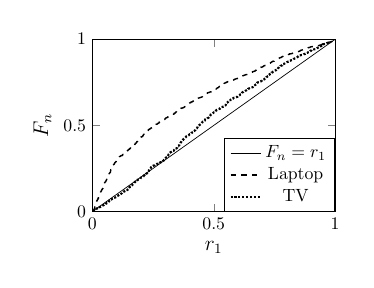
\begin{tikzpicture}[scale=0.64]
\begin{axis}[height=5cm,
width=6.4cm,
xmin=0,
xmax=1,
ymin=0,
ymax=1,legend style={at={(1,0)},anchor=south east},xlabel=$r_1$, ylabel=$F_n$,ylabel near ticks, xtick={0, 0.5, 1}, ytick={0, 0.5, 1}, label style={font=\large}, tick style={font=\Large}
]
\addplot+ [color=black,mark=none] coordinates {(0, 0) (0.5, 0.5) (1, 1)};
\addplot+ [color=black,mark=none,dashed,thick] coordinates
{(0.00406504065041,0.0010101010101)(0.00446428571429,0.0020202020202)(0.00490196078431,0.0030303030303)(0.00505050505051,0.00505050505051)(0.00510204081633,0.00606060606061)(0.00529100529101,0.00707070707071)(0.00564971751412,0.00808080808081)(0.00568181818182,0.00909090909091)(0.00625,0.010101010101)(0.00645161290323,0.0111111111111)(0.00833333333333,0.0161616161616)(0.00840336134454,0.0171717171717)(0.00892857142857,0.0191919191919)(0.00980392156863,0.020202020202)(0.00990099009901,0.0222222222222)(0.01,0.0242424242424)(0.010101010101,0.0252525252525)(0.0103092783505,0.0282828282828)(0.010752688172,0.030303030303)(0.010989010989,0.0323232323232)(0.0113636363636,0.0333333333333)(0.0117647058824,0.0343434343434)(0.0123456790123,0.0353535353535)(0.0125,0.0373737373737)(0.0127118644068,0.0383838383838)(0.012987012987,0.0393939393939)(0.0133333333333,0.040404040404)(0.0142857142857,0.0434343434343)(0.0143884892086,0.0454545454545)(0.014598540146,0.0464646464646)(0.0147058823529,0.0484848484848)(0.0151515151515,0.0494949494949)(0.0152671755725,0.0505050505051)(0.0165289256198,0.0515151515152)(0.0166666666667,0.0565656565657)(0.0169491525424,0.0575757575758)(0.0172413793103,0.0585858585859)(0.0173913043478,0.059595959596)(0.0176991150442,0.0606060606061)(0.0187969924812,0.0616161616162)(0.0188679245283,0.0626262626263)(0.0196078431373,0.0636363636364)(0.0199637023593,0.0646464646465)(0.0204081632653,0.0656565656566)(0.0207373271889,0.0666666666667)(0.0213675213675,0.0676767676768)(0.0214285714286,0.069696969697)(0.0217391304348,0.0707070707071)(0.0222222222222,0.0727272727273)(0.0243902439024,0.0737373737374)(0.0245901639344,0.0747474747475)(0.025,0.0808080808081)(0.0252100840336,0.0828282828283)(0.0253164556962,0.0858585858586)(0.0253807106599,0.0868686868687)(0.025641025641,0.0878787878788)(0.027027027027,0.0888888888889)(0.0277777777778,0.089898989899)(0.0285714285714,0.0929292929293)(0.0288461538462,0.0939393939394)(0.028880866426,0.0949494949495)(0.0291666666667,0.0959595959596)(0.0294117647059,0.0969696969697)(0.0299145299145,0.0979797979798)(0.03,0.10101010101)(0.030303030303,0.10202020202)(0.0314465408805,0.10303030303)(0.0320512820513,0.10404040404)(0.0322580645161,0.105050505051)(0.0327868852459,0.106060606061)(0.0333333333333,0.110101010101)(0.0336134453782,0.111111111111)(0.0338983050847,0.113131313131)(0.0344827586207,0.114141414141)(0.035175879397,0.115151515152)(0.0353159851301,0.116161616162)(0.0357142857143,0.118181818182)(0.037037037037,0.119191919192)(0.0375,0.120202020202)(0.0377358490566,0.122222222222)(0.0382165605096,0.123232323232)(0.0385756676558,0.124242424242)(0.0387596899225,0.125252525253)(0.0392156862745,0.126262626263)(0.0402298850575,0.127272727273)(0.040404040404,0.128282828283)(0.0406091370558,0.129292929293)(0.0416666666667,0.132323232323)(0.0423728813559,0.133333333333)(0.0434782608696,0.134343434343)(0.04375,0.135353535354)(0.0438596491228,0.136363636364)(0.0442477876106,0.137373737374)(0.0443037974684,0.138383838384)(0.0447154471545,0.139393939394)(0.0447368421053,0.140404040404)(0.045197740113,0.141414141414)(0.0454545454545,0.142424242424)(0.0461538461538,0.143434343434)(0.0465489566613,0.144444444444)(0.0481927710843,0.145454545455)(0.0490196078431,0.146464646465)(0.0493827160494,0.147474747475)(0.0494949494949,0.148484848485)(0.0495867768595,0.149494949495)(0.0496183206107,0.150505050505)(0.05,0.162626262626)(0.0502283105023,0.163636363636)(0.0503597122302,0.164646464646)(0.0506329113924,0.166666666667)(0.0508474576271,0.167676767677)(0.0520231213873,0.168686868687)(0.0522388059701,0.169696969697)(0.0526315789474,0.170707070707)(0.0527859237537,0.171717171717)(0.0545454545455,0.172727272727)(0.055,0.173737373737)(0.0552763819095,0.174747474747)(0.0554156171285,0.175757575758)(0.0558659217877,0.176767676768)(0.056,0.177777777778)(0.0563829787234,0.178787878788)(0.0571428571429,0.179797979798)(0.0575539568345,0.180808080808)(0.0579710144928,0.181818181818)(0.0583333333333,0.183838383838)(0.0588235294118,0.186868686869)(0.0594059405941,0.188888888889)(0.0596590909091,0.189898989899)(0.06,0.191919191919)(0.0604026845638,0.192929292929)(0.0607476635514,0.193939393939)(0.0617283950617,0.194949494949)(0.0632911392405,0.19595959596)(0.0641025641026,0.19696969697)(0.0651162790698,0.19797979798)(0.0652173913043,0.19898989899)(0.0655737704918,0.20101010101)(0.0657894736842,0.20202020202)(0.0660377358491,0.20303030303)(0.0661157024793,0.20404040404)(0.0666666666667,0.207070707071)(0.0672268907563,0.208080808081)(0.0675105485232,0.209090909091)(0.0676691729323,0.210101010101)(0.0677966101695,0.211111111111)(0.0681818181818,0.214141414141)(0.0683229813665,0.215151515152)(0.0683760683761,0.216161616162)(0.06875,0.218181818182)(0.0689655172414,0.219191919192)(0.0696202531646,0.220202020202)(0.07,0.221212121212)(0.0705882352941,0.222222222222)(0.0708661417323,0.223232323232)(0.0714285714286,0.224242424242)(0.0718562874251,0.225252525253)(0.0724637681159,0.226262626263)(0.0731707317073,0.227272727273)(0.0743405275779,0.228282828283)(0.0745341614907,0.229292929293)(0.0746268656716,0.230303030303)(0.075,0.235353535354)(0.0752688172043,0.236363636364)(0.0754716981132,0.237373737374)(0.0756302521008,0.238383838384)(0.0757575757576,0.239393939394)(0.0758928571429,0.240404040404)(0.0761421319797,0.241414141414)(0.0762711864407,0.242424242424)(0.0763358778626,0.243434343434)(0.0775862068966,0.244444444444)(0.0780399274047,0.245454545455)(0.0792079207921,0.246464646465)(0.0793650793651,0.247474747475)(0.08,0.248484848485)(0.0812324929972,0.249494949495)(0.08125,0.250505050505)(0.0819672131148,0.253535353535)(0.0828025477707,0.254545454545)(0.0840336134454,0.257575757576)(0.0844907407407,0.258585858586)(0.0847457627119,0.260606060606)(0.0849056603774,0.261616161616)(0.0849420849421,0.262626262626)(0.0849673202614,0.263636363636)(0.0851063829787,0.264646464646)(0.0857142857143,0.267676767677)(0.0858585858586,0.268686868687)(0.0869565217391,0.270707070707)(0.0875,0.271717171717)(0.0878661087866,0.272727272727)(0.0886075949367,0.273737373737)(0.0898617511521,0.274747474747)(0.09,0.275757575758)(0.0904977375566,0.276767676768)(0.0909090909091,0.278787878788)(0.0916666666667,0.280808080808)(0.0923076923077,0.281818181818)(0.0925925925926,0.282828282828)(0.0928571428571,0.283838383838)(0.0948275862069,0.285858585859)(0.0957446808511,0.286868686869)(0.0965909090909,0.287878787879)(0.0970873786408,0.288888888889)(0.0974358974359,0.289898989899)(0.0983606557377,0.290909090909)(0.1,0.29595959596)(0.100358422939,0.29696969697)(0.100529100529,0.29797979798)(0.100917431193,0.29898989899)(0.10101010101,0.3)(0.101234567901,0.30101010101)(0.103448275862,0.30202020202)(0.103896103896,0.30303030303)(0.10447761194,0.30404040404)(0.105,0.305050505051)(0.105555555556,0.306060606061)(0.105769230769,0.307070707071)(0.105882352941,0.308080808081)(0.10599078341,0.309090909091)(0.106299212598,0.310101010101)(0.106796116505,0.311111111111)(0.107142857143,0.312121212121)(0.108695652174,0.314141414141)(0.108860759494,0.315151515152)(0.11,0.316161616162)(0.110169491525,0.317171717172)(0.110552763819,0.318181818182)(0.1125,0.319191919192)(0.115,0.320202020202)(0.115384615385,0.321212121212)(0.116666666667,0.322222222222)(0.117647058824,0.323232323232)(0.118072289157,0.324242424242)(0.123188405797,0.325252525253)(0.123966942149,0.326262626263)(0.125,0.330303030303)(0.125925925926,0.331313131313)(0.12890625,0.332323232323)(0.130434782609,0.333333333333)(0.133333333333,0.336363636364)(0.133858267717,0.337373737374)(0.133928571429,0.338383838384)(0.134453781513,0.339393939394)(0.135593220339,0.341414141414)(0.135714285714,0.342424242424)(0.1375,0.343434343434)(0.137614678899,0.344444444444)(0.137931034483,0.345454545455)(0.13829787234,0.346464646465)(0.139784946237,0.347474747475)(0.14,0.348484848485)(0.140127388535,0.349494949495)(0.140287769784,0.350505050505)(0.141666666667,0.351515151515)(0.142857142857,0.352525252525)(0.145569620253,0.353535353535)(0.145631067961,0.354545454545)(0.146153846154,0.355555555556)(0.147058823529,0.356565656566)(0.148648648649,0.357575757576)(0.15,0.360606060606)(0.151898734177,0.361616161616)(0.15221402214,0.362626262626)(0.152542372881,0.363636363636)(0.153846153846,0.364646464646)(0.155555555556,0.365656565657)(0.155660377358,0.366666666667)(0.15625,0.367676767677)(0.157142857143,0.369696969697)(0.158273381295,0.370707070707)(0.158333333333,0.371717171717)(0.158536585366,0.372727272727)(0.16,0.373737373737)(0.160714285714,0.374747474747)(0.161779575329,0.375757575758)(0.163120567376,0.376767676768)(0.163204747774,0.377777777778)(0.163265306122,0.378787878788)(0.165254237288,0.379797979798)(0.165413533835,0.380808080808)(0.165467625899,0.381818181818)(0.166666666667,0.383838383838)(0.17,0.384848484848)(0.174273858921,0.385858585859)(0.174418604651,0.386868686869)(0.175,0.388888888889)(0.175273865415,0.389898989899)(0.175824175824,0.390909090909)(0.176,0.391919191919)(0.176470588235,0.392929292929)(0.17695473251,0.393939393939)(0.176991150442,0.394949494949)(0.177215189873,0.39595959596)(0.179487179487,0.39696969697)(0.180555555556,0.39797979798)(0.181034482759,0.39898989899)(0.181818181818,0.4)(0.182389937107,0.40101010101)(0.182481751825,0.40202020202)(0.183333333333,0.405050505051)(0.183673469388,0.406060606061)(0.185714285714,0.407070707071)(0.186440677966,0.408080808081)(0.186666666667,0.409090909091)(0.187050359712,0.410101010101)(0.1875,0.411111111111)(0.189189189189,0.412121212121)(0.189873417722,0.413131313131)(0.190045248869,0.414141414141)(0.191268191268,0.415151515152)(0.191666666667,0.416161616162)(0.191780821918,0.417171717172)(0.192307692308,0.418181818182)(0.19298245614,0.419191919192)(0.193277310924,0.420202020202)(0.194915254237,0.421212121212)(0.194968553459,0.422222222222)(0.195530726257,0.423232323232)(0.196261682243,0.424242424242)(0.196629213483,0.425252525253)(0.196721311475,0.426262626263)(0.199029126214,0.427272727273)(0.2,0.431313131313)(0.201219512195,0.432323232323)(0.201765447667,0.433333333333)(0.205555555556,0.434343434343)(0.206349206349,0.435353535354)(0.206611570248,0.436363636364)(0.206896551724,0.438383838384)(0.207650273224,0.439393939394)(0.209150326797,0.440404040404)(0.209302325581,0.441414141414)(0.209523809524,0.443434343434)(0.210526315789,0.445454545455)(0.211111111111,0.446464646465)(0.211267605634,0.447474747475)(0.2125,0.448484848485)(0.215517241379,0.449494949495)(0.215909090909,0.450505050505)(0.216666666667,0.456565656566)(0.217391304348,0.457575757576)(0.218487394958,0.458585858586)(0.2194092827,0.459595959596)(0.219653179191,0.460606060606)(0.222222222222,0.462626262626)(0.223300970874,0.464646464646)(0.224137931034,0.465656565657)(0.225,0.468686868687)(0.228070175439,0.469696969697)(0.229508196721,0.470707070707)(0.229571984436,0.471717171717)(0.22972972973,0.472727272727)(0.231481481481,0.473737373737)(0.231707317073,0.474747474747)(0.232558139535,0.475757575758)(0.233333333333,0.476767676768)(0.234375,0.477777777778)(0.23602484472,0.478787878788)(0.237288135593,0.479797979798)(0.238636363636,0.480808080808)(0.24,0.481818181818)(0.240740740741,0.483838383838)(0.242857142857,0.484848484848)(0.24375,0.485858585859)(0.245,0.486868686869)(0.246376811594,0.487878787879)(0.247706422018,0.488888888889)(0.25,0.490909090909)(0.251082251082,0.491919191919)(0.251533742331,0.492929292929)(0.251592356688,0.493939393939)(0.253968253968,0.494949494949)(0.256198347107,0.49595959596)(0.256544502618,0.49696969697)(0.257142857143,0.49797979798)(0.258992805755,0.49898989899)(0.26,0.5)(0.260162601626,0.50101010101)(0.261146496815,0.50202020202)(0.261538461538,0.50303030303)(0.262295081967,0.50404040404)(0.2625,0.506060606061)(0.265060240964,0.507070707071)(0.267045454545,0.508080808081)(0.267326732673,0.509090909091)(0.268115942029,0.510101010101)(0.268482490272,0.511111111111)(0.271739130435,0.512121212121)(0.273684210526,0.513131313131)(0.27397260274,0.514141414141)(0.274725274725,0.515151515152)(0.275,0.518181818182)(0.275449101796,0.519191919192)(0.277777777778,0.520202020202)(0.27868852459,0.521212121212)(0.281105990783,0.522222222222)(0.282051282051,0.523232323232)(0.283018867925,0.524242424242)(0.285714285714,0.525252525253)(0.287037037037,0.526262626263)(0.289855072464,0.527272727273)(0.29,0.528282828283)(0.292817679558,0.529292929293)(0.293103448276,0.530303030303)(0.295081967213,0.531313131313)(0.295652173913,0.533333333333)(0.296296296296,0.534343434343)(0.298701298701,0.535353535354)(0.3,0.539393939394)(0.301556420233,0.540404040404)(0.301675977654,0.541414141414)(0.302521008403,0.542424242424)(0.303571428571,0.543434343434)(0.304964539007,0.544444444444)(0.307971014493,0.545454545455)(0.308755760369,0.546464646465)(0.309523809524,0.547474747475)(0.31,0.548484848485)(0.3125,0.549494949495)(0.312727272727,0.550505050505)(0.313725490196,0.551515151515)(0.313829787234,0.552525252525)(0.315315315315,0.553535353535)(0.317901234568,0.554545454545)(0.318918918919,0.555555555556)(0.32,0.556565656566)(0.320512820513,0.557575757576)(0.321626617375,0.558585858586)(0.322115384615,0.559595959596)(0.322784810127,0.560606060606)(0.324137931034,0.561616161616)(0.326086956522,0.562626262626)(0.327044025157,0.563636363636)(0.332214765101,0.564646464646)(0.335443037975,0.565656565657)(0.335664335664,0.566666666667)(0.337579617834,0.567676767677)(0.337662337662,0.568686868687)(0.337704918033,0.569696969697)(0.337837837838,0.570707070707)(0.341176470588,0.571717171717)(0.341666666667,0.572727272727)(0.342105263158,0.573737373737)(0.34328358209,0.574747474747)(0.343434343434,0.575757575758)(0.343511450382,0.576767676768)(0.345132743363,0.577777777778)(0.345864661654,0.578787878788)(0.346774193548,0.579797979798)(0.347457627119,0.581818181818)(0.347826086957,0.582828282828)(0.35,0.584848484848)(0.350806451613,0.585858585859)(0.351063829787,0.586868686869)(0.352941176471,0.587878787879)(0.354085603113,0.588888888889)(0.355263157895,0.589898989899)(0.35593220339,0.590909090909)(0.356164383562,0.591919191919)(0.35625,0.592929292929)(0.357142857143,0.593939393939)(0.357664233577,0.594949494949)(0.3625,0.59595959596)(0.364285714286,0.59797979798)(0.36443148688,0.59898989899)(0.366666666667,0.6)(0.370786516854,0.60101010101)(0.372727272727,0.60202020202)(0.375,0.60303030303)(0.377049180328,0.60404040404)(0.378378378378,0.606060606061)(0.379182156134,0.607070707071)(0.380281690141,0.608080808081)(0.381818181818,0.609090909091)(0.383084577114,0.610101010101)(0.384615384615,0.611111111111)(0.385964912281,0.612121212121)(0.388157894737,0.613131313131)(0.388329979879,0.614141414141)(0.388888888889,0.615151515152)(0.39,0.616161616162)(0.391666666667,0.618181818182)(0.39175257732,0.619191919192)(0.393162393162,0.620202020202)(0.39375,0.621212121212)(0.393939393939,0.622222222222)(0.394871794872,0.623232323232)(0.395280235988,0.624242424242)(0.397260273973,0.625252525253)(0.397435897436,0.626262626263)(0.4,0.629292929293)(0.401639344262,0.630303030303)(0.403314917127,0.631313131313)(0.40503875969,0.632323232323)(0.40625,0.633333333333)(0.406451612903,0.634343434343)(0.406593406593,0.635353535354)(0.410447761194,0.636363636364)(0.410714285714,0.637373737374)(0.4125,0.638383838384)(0.4140625,0.639393939394)(0.415094339623,0.641414141414)(0.416464891041,0.642424242424)(0.417721518987,0.643434343434)(0.418972332016,0.644444444444)(0.42328042328,0.645454545455)(0.424778761062,0.646464646465)(0.425,0.648484848485)(0.427536231884,0.649494949495)(0.428217821782,0.650505050505)(0.428571428571,0.651515151515)(0.429447852761,0.652525252525)(0.42962962963,0.653535353535)(0.43,0.654545454545)(0.432432432432,0.655555555556)(0.433121019108,0.656565656566)(0.433155080214,0.657575757576)(0.44,0.659595959596)(0.441666666667,0.660606060606)(0.444444444444,0.661616161616)(0.446022727273,0.662626262626)(0.448275862069,0.663636363636)(0.450819672131,0.664646464646)(0.452261306533,0.665656565657)(0.453608247423,0.666666666667)(0.453781512605,0.667676767677)(0.454545454545,0.669696969697)(0.455555555556,0.670707070707)(0.456375838926,0.671717171717)(0.459183673469,0.672727272727)(0.46,0.673737373737)(0.460317460317,0.674747474747)(0.460526315789,0.675757575758)(0.460869565217,0.676767676768)(0.461538461538,0.677777777778)(0.463235294118,0.678787878788)(0.466666666667,0.680808080808)(0.467532467532,0.681818181818)(0.46835443038,0.682828282828)(0.469026548673,0.683838383838)(0.469101123596,0.684848484848)(0.470967741935,0.685858585859)(0.473214285714,0.686868686869)(0.473451327434,0.687878787879)(0.474226804124,0.688888888889)(0.477272727273,0.689898989899)(0.480519480519,0.690909090909)(0.481865284974,0.691919191919)(0.483050847458,0.692929292929)(0.483660130719,0.693939393939)(0.488888888889,0.694949494949)(0.491666666667,0.69595959596)(0.492537313433,0.69696969697)(0.492753623188,0.69898989899)(0.493150684932,0.7)(0.493506493506,0.70101010101)(0.493617021277,0.70202020202)(0.494339622642,0.70303030303)(0.495412844037,0.70404040404)(0.49880952381,0.705050505051)(0.5,0.708080808081)(0.502793296089,0.709090909091)(0.503267973856,0.710101010101)(0.509433962264,0.711111111111)(0.510791366906,0.712121212121)(0.510948905109,0.713131313131)(0.511627906977,0.714141414141)(0.5125,0.715151515152)(0.513447432763,0.716161616162)(0.514492753623,0.717171717172)(0.516129032258,0.718181818182)(0.518518518519,0.719191919192)(0.519480519481,0.720202020202)(0.52,0.721212121212)(0.520547945205,0.722222222222)(0.521452145215,0.723232323232)(0.522388059701,0.724242424242)(0.522522522523,0.725252525253)(0.525252525253,0.726262626263)(0.530864197531,0.727272727273)(0.533898305085,0.728282828283)(0.534090909091,0.730303030303)(0.534482758621,0.731313131313)(0.535123966942,0.732323232323)(0.537459283388,0.733333333333)(0.537572254335,0.734343434343)(0.538461538462,0.735353535354)(0.54,0.736363636364)(0.540816326531,0.737373737374)(0.541095890411,0.738383838384)(0.541899441341,0.739393939394)(0.542253521127,0.740404040404)(0.542372881356,0.741414141414)(0.542635658915,0.742424242424)(0.54347826087,0.744444444444)(0.545454545455,0.745454545455)(0.547169811321,0.746464646465)(0.547619047619,0.747474747475)(0.550458715596,0.748484848485)(0.550724637681,0.749494949495)(0.554347826087,0.750505050505)(0.554455445545,0.751515151515)(0.554817275748,0.752525252525)(0.556962025316,0.753535353535)(0.56,0.754545454545)(0.5625,0.755555555556)(0.563636363636,0.756565656566)(0.568888888889,0.757575757576)(0.568965517241,0.758585858586)(0.569060773481,0.759595959596)(0.571428571429,0.760606060606)(0.576923076923,0.761616161616)(0.577968526466,0.762626262626)(0.581818181818,0.763636363636)(0.583333333333,0.764646464646)(0.583643122677,0.765656565657)(0.584569732938,0.766666666667)(0.585858585859,0.767676767677)(0.588888888889,0.768686868687)(0.590361445783,0.769696969697)(0.591666666667,0.770707070707)(0.595505617978,0.771717171717)(0.59793814433,0.772727272727)(0.601895734597,0.773737373737)(0.602272727273,0.774747474747)(0.602510460251,0.775757575758)(0.602941176471,0.776767676768)(0.603448275862,0.777777777778)(0.604761904762,0.778787878788)(0.606060606061,0.779797979798)(0.606936416185,0.780808080808)(0.607142857143,0.781818181818)(0.61038961039,0.782828282828)(0.612068965517,0.783838383838)(0.612385321101,0.784848484848)(0.614457831325,0.785858585859)(0.618421052632,0.787878787879)(0.622222222222,0.788888888889)(0.624338624339,0.789898989899)(0.625,0.790909090909)(0.626373626374,0.791919191919)(0.630136986301,0.792929292929)(0.630769230769,0.793939393939)(0.633928571429,0.794949494949)(0.638157894737,0.79595959596)(0.64,0.79696969697)(0.640909090909,0.79797979798)(0.641304347826,0.79898989899)(0.641666666667,0.8)(0.642857142857,0.80101010101)(0.650406504065,0.80202020202)(0.651595744681,0.80303030303)(0.65243902439,0.80404040404)(0.653846153846,0.805050505051)(0.654205607477,0.806060606061)(0.656862745098,0.807070707071)(0.657534246575,0.808080808081)(0.659090909091,0.809090909091)(0.659722222222,0.810101010101)(0.660869565217,0.811111111111)(0.661016949153,0.812121212121)(0.666666666667,0.814141414141)(0.669811320755,0.815151515152)(0.67,0.816161616162)(0.670454545455,0.817171717172)(0.671641791045,0.818181818182)(0.672077922078,0.819191919192)(0.673913043478,0.820202020202)(0.675,0.821212121212)(0.675126903553,0.822222222222)(0.676470588235,0.823232323232)(0.676767676768,0.824242424242)(0.677419354839,0.825252525253)(0.677966101695,0.826262626263)(0.678899082569,0.827272727273)(0.679245283019,0.828282828283)(0.679487179487,0.829292929293)(0.68115942029,0.830303030303)(0.683544303797,0.831313131313)(0.685483870968,0.832323232323)(0.6875,0.833333333333)(0.688559322034,0.834343434343)(0.691666666667,0.835353535354)(0.693693693694,0.836363636364)(0.69375,0.837373737374)(0.698275862069,0.838383838384)(0.7,0.839393939394)(0.701030927835,0.840404040404)(0.70297029703,0.841414141414)(0.703832752613,0.842424242424)(0.704402515723,0.843434343434)(0.705882352941,0.844444444444)(0.70625,0.845454545455)(0.708955223881,0.846464646465)(0.711111111111,0.847474747475)(0.71186440678,0.848484848485)(0.715909090909,0.849494949495)(0.716666666667,0.850505050505)(0.71875,0.852525252525)(0.719101123596,0.853535353535)(0.721518987342,0.854545454545)(0.72197309417,0.855555555556)(0.722222222222,0.856565656566)(0.722772277228,0.857575757576)(0.729323308271,0.858585858586)(0.730769230769,0.859595959596)(0.731958762887,0.860606060606)(0.733333333333,0.862626262626)(0.73417721519,0.863636363636)(0.734375,0.864646464646)(0.736111111111,0.865656565657)(0.737373737374,0.866666666667)(0.73786407767,0.867676767677)(0.740088105727,0.868686868687)(0.740740740741,0.869696969697)(0.741379310345,0.870707070707)(0.741935483871,0.871717171717)(0.748427672956,0.872727272727)(0.748603351955,0.873737373737)(0.75,0.875757575758)(0.752475247525,0.876767676768)(0.752688172043,0.877777777778)(0.754716981132,0.878787878788)(0.756097560976,0.879797979798)(0.757142857143,0.880808080808)(0.758620689655,0.881818181818)(0.758865248227,0.882828282828)(0.760563380282,0.883838383838)(0.7625,0.884848484848)(0.764227642276,0.885858585859)(0.766233766234,0.886868686869)(0.767123287671,0.887878787879)(0.768115942029,0.888888888889)(0.769230769231,0.889898989899)(0.769736842105,0.890909090909)(0.771428571429,0.891919191919)(0.773480662983,0.892929292929)(0.776978417266,0.893939393939)(0.778523489933,0.894949494949)(0.778571428571,0.89595959596)(0.779661016949,0.89696969697)(0.78064516129,0.89797979798)(0.782051282051,0.89898989899)(0.784615384615,0.9)(0.785123966942,0.90101010101)(0.786324786325,0.90202020202)(0.787234042553,0.90303030303)(0.7875,0.90404040404)(0.79012345679,0.905050505051)(0.801724137931,0.906060606061)(0.803418803419,0.907070707071)(0.805194805195,0.908080808081)(0.806930693069,0.909090909091)(0.807142857143,0.910101010101)(0.808333333333,0.911111111111)(0.808510638298,0.912121212121)(0.811320754717,0.913131313131)(0.8125,0.915151515152)(0.818181818182,0.916161616162)(0.821428571429,0.917171717172)(0.824561403509,0.918181818182)(0.825,0.919191919192)(0.828571428571,0.920202020202)(0.830508474576,0.922222222222)(0.831168831169,0.923232323232)(0.836363636364,0.924242424242)(0.838709677419,0.925252525253)(0.842592592593,0.926262626263)(0.846153846154,0.927272727273)(0.848101265823,0.928282828283)(0.85,0.929292929293)(0.852534562212,0.930303030303)(0.85401459854,0.931313131313)(0.854545454545,0.932323232323)(0.856164383562,0.933333333333)(0.857142857143,0.934343434343)(0.858974358974,0.936363636364)(0.861538461538,0.937373737374)(0.866666666667,0.938383838384)(0.869318181818,0.939393939394)(0.869565217391,0.940404040404)(0.871794871795,0.941414141414)(0.873873873874,0.942424242424)(0.87610619469,0.943434343434)(0.876712328767,0.944444444444)(0.878787878788,0.945454545455)(0.882352941176,0.947474747475)(0.885964912281,0.948484848485)(0.887096774194,0.949494949495)(0.888172043011,0.950505050505)(0.890410958904,0.951515151515)(0.893280632411,0.952525252525)(0.896907216495,0.953535353535)(0.897959183673,0.954545454545)(0.898785425101,0.955555555556)(0.9,0.956565656566)(0.910714285714,0.957575757576)(0.9125,0.958585858586)(0.920168067227,0.959595959596)(0.924369747899,0.960606060606)(0.925,0.961616161616)(0.926229508197,0.962626262626)(0.933333333333,0.963636363636)(0.93625498008,0.964646464646)(0.936507936508,0.965656565657)(0.938775510204,0.966666666667)(0.942857142857,0.967676767677)(0.945392491468,0.968686868687)(0.945454545455,0.969696969697)(0.945945945946,0.970707070707)(0.949579831933,0.971717171717)(0.95,0.972727272727)(0.955555555556,0.973737373737)(0.958333333333,0.975757575758)(0.96,0.976767676768)(0.960264900662,0.977777777778)(0.962264150943,0.978787878788)(0.965217391304,0.979797979798)(0.966666666667,0.980808080808)(0.974358974359,0.981818181818)(0.974789915966,0.982828282828)(0.975,0.983838383838)(0.983050847458,0.984848484848)(0.985,0.985858585859)(0.985714285714,0.986868686869)(0.987951807229,0.987878787879)(0.99,0.988888888889)(0.991666666667,0.989898989899)(1.0,1.0)};
\addplot+ [color=black,mark=none,densely dotted, very thick] coordinates
{(0.003861003861,0.00100300902708)(0.00625,0.00200601805416)(0.00632911392405,0.00300902708124)(0.0077519379845,0.00401203610832)(0.00833333333333,0.00501504513541)(0.00862068965517,0.00601805416249)(0.00892857142857,0.00702106318957)(0.0104166666667,0.00802407221665)(0.0106382978723,0.00902708124373)(0.0119047619048,0.0100300902708)(0.0125,0.0110330992979)(0.0133333333333,0.012036108325)(0.0148514851485,0.0130391173521)(0.0151515151515,0.0140421263791)(0.0166666666667,0.0150451354062)(0.0167597765363,0.0160481444333)(0.0169491525424,0.0170511534604)(0.02,0.0180541624875)(0.0201005025126,0.0190571715145)(0.0252100840336,0.0200601805416)(0.025974025974,0.0210631895687)(0.0264317180617,0.0220661985958)(0.027027027027,0.0240722166499)(0.0298507462687,0.025075225677)(0.03,0.0260782347041)(0.0333333333333,0.0270812437312)(0.0336134453782,0.0280842527583)(0.0344827586207,0.0290872617854)(0.0363636363636,0.0300902708124)(0.0380952380952,0.0310932798395)(0.0381679389313,0.0320962888666)(0.04,0.0330992978937)(0.0413223140496,0.0341023069208)(0.0416666666667,0.0351053159478)(0.0453257790368,0.0361083249749)(0.0463768115942,0.037111334002)(0.048,0.0381143430291)(0.0491071428571,0.0391173520562)(0.0493421052632,0.0401203610832)(0.0493827160494,0.0411233701103)(0.05,0.0421263791374)(0.0503597122302,0.0431293881645)(0.0542168674699,0.0441323971916)(0.054347826087,0.0451354062187)(0.0574712643678,0.0461384152457)(0.0583333333333,0.0471414242728)(0.0588235294118,0.0481444332999)(0.06,0.049147442327)(0.0625,0.0501504513541)(0.0636363636364,0.0511534603811)(0.0642857142857,0.0531594784353)(0.0666666666667,0.0541624874624)(0.0671641791045,0.0551654964895)(0.0672268907563,0.0561685055165)(0.0677966101695,0.0571715145436)(0.0686274509804,0.0581745235707)(0.0689655172414,0.0601805416249)(0.0695652173913,0.061183550652)(0.07,0.0631895687061)(0.0701986754967,0.0641925777332)(0.0714285714286,0.0651955867603)(0.0754716981132,0.0661985957874)(0.0756302521008,0.0682046138415)(0.0757575757576,0.0692076228686)(0.0785714285714,0.0702106318957)(0.0792079207921,0.0712136409228)(0.08,0.0722166499498)(0.0817610062893,0.0732196589769)(0.0838323353293,0.074222668004)(0.0859375,0.0752256770311)(0.0864197530864,0.0762286860582)(0.0886075949367,0.0772316950853)(0.0888888888889,0.0782347041123)(0.0891089108911,0.0792377131394)(0.0892857142857,0.0802407221665)(0.0943396226415,0.0812437311936)(0.0955882352941,0.0822467402207)(0.0967741935484,0.0832497492477)(0.0983606557377,0.0842527582748)(0.0993377483444,0.0852557673019)(0.1,0.0872617853561)(0.100358422939,0.0882647943831)(0.101351351351,0.0892678034102)(0.102564102564,0.0902708124373)(0.104395604396,0.0912738214644)(0.105,0.0922768304915)(0.107692307692,0.0932798395186)(0.108312342569,0.0942828485456)(0.108333333333,0.0952858575727)(0.110344827586,0.0962888665998)(0.11038961039,0.0972918756269)(0.110599078341,0.098294884654)(0.114285714286,0.099297893681)(0.115789473684,0.100300902708)(0.117117117117,0.101303911735)(0.117647058824,0.102306920762)(0.11875,0.103309929789)(0.119266055046,0.104312938816)(0.12,0.105315947844)(0.121621621622,0.106318956871)(0.122529644269,0.107321965898)(0.123028391167,0.108324974925)(0.125,0.11334002006)(0.127272727273,0.114343029087)(0.127777777778,0.115346038114)(0.131818181818,0.116349047141)(0.131926121372,0.117352056169)(0.132530120482,0.118355065196)(0.133004926108,0.119358074223)(0.133333333333,0.121364092277)(0.137931034483,0.122367101304)(0.139240506329,0.123370110331)(0.140350877193,0.124373119358)(0.144144144144,0.125376128385)(0.14465408805,0.126379137412)(0.145098039216,0.127382146439)(0.146118721461,0.128385155466)(0.148148148148,0.130391173521)(0.148936170213,0.131394182548)(0.149068322981,0.132397191575)(0.149171270718,0.133400200602)(0.149253731343,0.134403209629)(0.15,0.135406218656)(0.150442477876,0.136409227683)(0.150943396226,0.139418254764)(0.152671755725,0.140421263791)(0.15306122449,0.141424272818)(0.154545454545,0.142427281846)(0.154929577465,0.1444332999)(0.155555555556,0.146439317954)(0.158415841584,0.147442326981)(0.15873015873,0.148445336008)(0.16091954023,0.149448345035)(0.161111111111,0.150451354062)(0.162162162162,0.151454363089)(0.1625,0.152457372116)(0.164179104478,0.153460381143)(0.165217391304,0.154463390171)(0.165467625899,0.156469408225)(0.165829145729,0.157472417252)(0.166666666667,0.158475426279)(0.167597765363,0.159478435306)(0.168674698795,0.160481444333)(0.169491525424,0.16148445336)(0.169811320755,0.162487462387)(0.17,0.164493480441)(0.172413793103,0.165496489468)(0.172727272727,0.166499498495)(0.173228346457,0.167502507523)(0.173469387755,0.16850551655)(0.175,0.169508525577)(0.175438596491,0.170511534604)(0.176100628931,0.172517552658)(0.176470588235,0.173520561685)(0.178294573643,0.174523570712)(0.178571428571,0.175526579739)(0.18,0.176529588766)(0.181034482759,0.177532597793)(0.181818181818,0.17853560682)(0.18253968254,0.179538615848)(0.183333333333,0.181544633902)(0.185840707965,0.182547642929)(0.186666666667,0.183550651956)(0.186781609195,0.184553660983)(0.189189189189,0.18555667001)(0.191616766467,0.186559679037)(0.19298245614,0.187562688064)(0.19512195122,0.188565697091)(0.195652173913,0.189568706118)(0.197530864198,0.190571715145)(0.19801980198,0.191574724173)(0.198198198198,0.1925777332)(0.198412698413,0.193580742227)(0.2,0.196589769308)(0.201438848921,0.197592778335)(0.202614379085,0.198595787362)(0.205555555556,0.199598796389)(0.206611570248,0.200601805416)(0.207207207207,0.201604814443)(0.208333333333,0.20260782347)(0.209944751381,0.203610832497)(0.21,0.204613841525)(0.2100456621,0.205616850552)(0.210526315789,0.206619859579)(0.212389380531,0.207622868606)(0.212765957447,0.208625877633)(0.213636363636,0.20962888666)(0.213836477987,0.210631895687)(0.215384615385,0.211634904714)(0.215517241379,0.212637913741)(0.216666666667,0.214643931795)(0.219594594595,0.215646940822)(0.22,0.21664994985)(0.220588235294,0.217652958877)(0.220779220779,0.218655967904)(0.222222222222,0.219658976931)(0.224137931034,0.221664994985)(0.22641509434,0.222668004012)(0.227036395147,0.223671013039)(0.227941176471,0.224674022066)(0.228169014085,0.225677031093)(0.228260869565,0.22668004012)(0.228758169935,0.227683049147)(0.229885057471,0.228686058175)(0.230769230769,0.230692076229)(0.231759656652,0.231695085256)(0.232142857143,0.23370110331)(0.232673267327,0.234704112337)(0.232876712329,0.235707121364)(0.233333333333,0.240722166499)(0.233766233766,0.241725175527)(0.23417721519,0.242728184554)(0.234636871508,0.243731193581)(0.235294117647,0.245737211635)(0.236180904523,0.246740220662)(0.236559139785,0.247743229689)(0.237288135593,0.248746238716)(0.237442922374,0.249749247743)(0.2375,0.25075225677)(0.24,0.251755265797)(0.240458015267,0.252758274824)(0.240663900415,0.253761283852)(0.240740740741,0.254764292879)(0.241666666667,0.256770310933)(0.242990654206,0.25777331996)(0.243636363636,0.258776328987)(0.244635193133,0.259779338014)(0.245810055866,0.260782347041)(0.247663551402,0.261785356068)(0.25,0.265797392177)(0.254054054054,0.266800401204)(0.254237288136,0.267803410231)(0.25641025641,0.268806419258)(0.256756756757,0.269809428285)(0.257142857143,0.270812437312)(0.258333333333,0.271815446339)(0.259259259259,0.272818455366)(0.260162601626,0.273821464393)(0.262711864407,0.27482447342)(0.263888888889,0.275827482447)(0.266666666667,0.276830491474)(0.270833333333,0.277833500502)(0.271428571429,0.278836509529)(0.2734082397,0.279839518556)(0.275,0.280842527583)(0.277777777778,0.28184553661)(0.278481012658,0.282848545637)(0.278571428571,0.283851554664)(0.279279279279,0.284854563691)(0.279569892473,0.285857572718)(0.281553398058,0.286860581745)(0.286486486486,0.287863590772)(0.286666666667,0.288866599799)(0.286764705882,0.289869608826)(0.288288288288,0.290872617854)(0.291262135922,0.291875626881)(0.291666666667,0.293881644935)(0.292929292929,0.294884653962)(0.293413173653,0.295887662989)(0.294444444444,0.296890672016)(0.294642857143,0.297893681043)(0.294871794872,0.29889669007)(0.295081967213,0.299899699097)(0.296089385475,0.300902708124)(0.29702970297,0.301905717151)(0.298850574713,0.302908726179)(0.3,0.308926780341)(0.300751879699,0.309929789368)(0.301587301587,0.310932798395)(0.302325581395,0.311935807422)(0.303797468354,0.312938816449)(0.305084745763,0.313941825476)(0.305194805195,0.314944834504)(0.306930693069,0.315947843531)(0.307142857143,0.317953861585)(0.307692307692,0.319959879639)(0.309368191721,0.320962888666)(0.31,0.321965897693)(0.310344827586,0.32296890672)(0.310606060606,0.323971915747)(0.311926605505,0.324974924774)(0.3125,0.326980942828)(0.313043478261,0.327983951856)(0.313559322034,0.328986960883)(0.313725490196,0.32998996991)(0.313953488372,0.330992978937)(0.314285714286,0.331995987964)(0.314606741573,0.332998996991)(0.315315315315,0.334002006018)(0.316239316239,0.335005015045)(0.316666666667,0.337011033099)(0.317757009346,0.339017051153)(0.318548387097,0.340020060181)(0.32,0.341023069208)(0.320512820513,0.342026078235)(0.320987654321,0.343029087262)(0.321428571429,0.344032096289)(0.322033898305,0.345035105316)(0.324873096447,0.346038114343)(0.325925925926,0.34704112337)(0.326530612245,0.348044132397)(0.328244274809,0.349047141424)(0.329113924051,0.350050150451)(0.330357142857,0.351053159478)(0.330508474576,0.352056168506)(0.335195530726,0.353059177533)(0.335714285714,0.35406218656)(0.335820895522,0.355065195587)(0.336492890995,0.356068204614)(0.336787564767,0.357071213641)(0.336956521739,0.358074222668)(0.3375,0.359077231695)(0.338235294118,0.360080240722)(0.338461538462,0.362086258776)(0.34188034188,0.363089267803)(0.34375,0.36409227683)(0.344262295082,0.365095285858)(0.346153846154,0.366098294885)(0.34693877551,0.367101303912)(0.347457627119,0.368104312939)(0.349206349206,0.370110330993)(0.349557522124,0.37111334002)(0.349845201238,0.372116349047)(0.35,0.377131394183)(0.350877192982,0.37813440321)(0.351851851852,0.379137412237)(0.352490421456,0.380140421264)(0.354838709677,0.381143430291)(0.355555555556,0.382146439318)(0.356164383562,0.383149448345)(0.356435643564,0.384152457372)(0.357894736842,0.385155466399)(0.358695652174,0.387161484453)(0.36,0.392176529589)(0.36038961039,0.393179538616)(0.361111111111,0.394182547643)(0.361538461538,0.39518555667)(0.361842105263,0.396188565697)(0.36231884058,0.397191574724)(0.3625,0.398194583751)(0.363636363636,0.400200601805)(0.365,0.401203610832)(0.365546218487,0.40220661986)(0.365671641791,0.403209628887)(0.365853658537,0.404212637914)(0.366197183099,0.405215646941)(0.36676217765,0.406218655968)(0.367346938776,0.408224674022)(0.367521367521,0.409227683049)(0.367924528302,0.410230692076)(0.368421052632,0.411233701103)(0.37,0.41223671013)(0.371794871795,0.413239719157)(0.372093023256,0.414242728185)(0.373134328358,0.415245737212)(0.373333333333,0.416248746239)(0.373417721519,0.417251755266)(0.374613003096,0.418254764293)(0.375,0.420260782347)(0.375838926174,0.421263791374)(0.377192982456,0.422266800401)(0.378378378378,0.424272818455)(0.379746835443,0.425275827482)(0.380952380952,0.427281845537)(0.381679389313,0.428284854564)(0.382428940568,0.429287863591)(0.384615384615,0.431293881645)(0.384831460674,0.432296890672)(0.385,0.433299899699)(0.385542168675,0.434302908726)(0.385964912281,0.435305917753)(0.3875,0.43630892678)(0.388059701493,0.437311935807)(0.389830508475,0.438314944835)(0.391304347826,0.439317953862)(0.392156862745,0.440320962889)(0.393442622951,0.441323971916)(0.396551724138,0.442326980943)(0.397058823529,0.44332998997)(0.397959183673,0.444332998997)(0.39837398374,0.445336008024)(0.4,0.448345035105)(0.403361344538,0.449348044132)(0.40350877193,0.450351053159)(0.405405405405,0.451354062187)(0.405660377358,0.452357071214)(0.407407407407,0.453360080241)(0.407894736842,0.454363089268)(0.408163265306,0.455366098295)(0.408284023669,0.456369107322)(0.410071942446,0.457372116349)(0.410256410256,0.458375125376)(0.412280701754,0.459378134403)(0.415384615385,0.46038114343)(0.415492957746,0.461384152457)(0.415887850467,0.462387161484)(0.416243654822,0.463390170512)(0.416666666667,0.466399197593)(0.419047619048,0.46740220662)(0.419811320755,0.468405215647)(0.421686746988,0.469408224674)(0.422222222222,0.470411233701)(0.422680412371,0.471414242728)(0.423529411765,0.472417251755)(0.424581005587,0.473420260782)(0.424892703863,0.474423269809)(0.425,0.475426278837)(0.425196850394,0.476429287864)(0.425925925926,0.478435305918)(0.426966292135,0.479438314945)(0.428571428571,0.481444332999)(0.429487179487,0.482447342026)(0.43023255814,0.483450351053)(0.430769230769,0.48445336008)(0.43137254902,0.485456369107)(0.431818181818,0.486459378134)(0.433333333333,0.490471414243)(0.433962264151,0.49147442327)(0.434108527132,0.492477432297)(0.434210526316,0.493480441324)(0.434426229508,0.494483450351)(0.434782608696,0.495486459378)(0.435,0.496489468405)(0.4375,0.498495486459)(0.438596491228,0.499498495486)(0.439024390244,0.500501504514)(0.44094488189,0.501504513541)(0.441666666667,0.502507522568)(0.442477876106,0.503510531595)(0.443037974684,0.504513540622)(0.444029850746,0.505516549649)(0.444444444444,0.506519558676)(0.445454545455,0.507522567703)(0.446043165468,0.50852557673)(0.447368421053,0.509528585757)(0.447852760736,0.510531594784)(0.449152542373,0.511534603811)(0.45,0.513540621866)(0.450381679389,0.514543630893)(0.452054794521,0.517552657974)(0.453488372093,0.518555667001)(0.454545454545,0.521564694082)(0.457627118644,0.522567703109)(0.458181818182,0.523570712136)(0.46,0.524573721163)(0.460526315789,0.526579739218)(0.46256684492,0.527582748245)(0.463414634146,0.528585757272)(0.463541666667,0.529588766299)(0.464285714286,0.53259779338)(0.464646464646,0.533600802407)(0.464751958225,0.534603811434)(0.467153284672,0.535606820461)(0.46875,0.536609829488)(0.469387755102,0.537612838516)(0.471698113208,0.538615847543)(0.472972972973,0.53961885657)(0.473282442748,0.540621865597)(0.473602484472,0.541624874624)(0.475935828877,0.542627883651)(0.476923076923,0.543630892678)(0.478260869565,0.544633901705)(0.478991596639,0.545636910732)(0.480519480519,0.546639919759)(0.480662983425,0.547642928786)(0.481481481481,0.549648946841)(0.482352941176,0.550651955868)(0.483333333333,0.553660982949)(0.483870967742,0.554663991976)(0.48427672956,0.555667001003)(0.484848484848,0.55667001003)(0.486842105263,0.558676028084)(0.487394957983,0.560682046138)(0.4875,0.562688064193)(0.489847715736,0.56369107322)(0.490683229814,0.564694082247)(0.491525423729,0.565697091274)(0.492753623188,0.566700100301)(0.49377593361,0.567703109328)(0.5,0.575727181545)(0.50303030303,0.576730190572)(0.503184713376,0.577733199599)(0.504587155963,0.578736208626)(0.50495049505,0.579739217653)(0.505882352941,0.58074222668)(0.506172839506,0.582748244734)(0.507772020725,0.583751253761)(0.508064516129,0.584754262788)(0.508196721311,0.585757271815)(0.509259259259,0.586760280843)(0.511450381679,0.58776328987)(0.511904761905,0.588766298897)(0.5125,0.589769307924)(0.515151515152,0.590772316951)(0.516666666667,0.591775325978)(0.516949152542,0.592778335005)(0.52,0.594784353059)(0.525,0.596790371113)(0.525139664804,0.59779338014)(0.525252525253,0.598796389168)(0.525316455696,0.599799398195)(0.526315789474,0.600802407222)(0.52688172043,0.601805416249)(0.527272727273,0.602808425276)(0.527868852459,0.603811434303)(0.529411764706,0.60481444333)(0.530120481928,0.605817452357)(0.533333333333,0.606820461384)(0.53781512605,0.607823470411)(0.538461538462,0.608826479438)(0.540540540541,0.609829488465)(0.540816326531,0.610832497492)(0.541176470588,0.61183550652)(0.54128440367,0.612838515547)(0.542168674699,0.613841524574)(0.542372881356,0.614844533601)(0.545454545455,0.615847542628)(0.548387096774,0.616850551655)(0.548872180451,0.617853560682)(0.54954954955,0.618856569709)(0.549645390071,0.619859578736)(0.55,0.622868605817)(0.550458715596,0.623871614845)(0.550505050505,0.624874623872)(0.550561797753,0.625877632899)(0.550724637681,0.626880641926)(0.550847457627,0.627883650953)(0.551181102362,0.62888665998)(0.552419354839,0.629889669007)(0.552631578947,0.630892678034)(0.554347826087,0.631895687061)(0.556603773585,0.632898696088)(0.557142857143,0.633901705115)(0.557692307692,0.634904714142)(0.559090909091,0.63590772317)(0.559322033898,0.637913741224)(0.56,0.638916750251)(0.561403508772,0.639919759278)(0.5625,0.640922768305)(0.56338028169,0.641925777332)(0.563636363636,0.643931795386)(0.564102564103,0.644934804413)(0.564220183486,0.64593781344)(0.56880733945,0.646940822467)(0.568965517241,0.648946840522)(0.569721115538,0.649949849549)(0.571428571429,0.650952858576)(0.572327044025,0.651955867603)(0.57264957265,0.65295887663)(0.575757575758,0.653961885657)(0.578571428571,0.654964894684)(0.579439252336,0.655967903711)(0.58,0.657973921765)(0.58125,0.658976930792)(0.581560283688,0.659979939819)(0.586956521739,0.660982948847)(0.590436590437,0.661985957874)(0.591304347826,0.662988966901)(0.593073593074,0.663991975928)(0.594202898551,0.664994984955)(0.597014925373,0.665997993982)(0.598326359833,0.667001003009)(0.6,0.67001003009)(0.603174603175,0.671013039117)(0.603603603604,0.672016048144)(0.604278074866,0.673019057172)(0.60447761194,0.674022066199)(0.606280193237,0.675025075226)(0.606666666667,0.676028084253)(0.607407407407,0.67703109328)(0.607476635514,0.678034102307)(0.608333333333,0.679037111334)(0.610526315789,0.680040120361)(0.613382899628,0.681043129388)(0.613445378151,0.682046138415)(0.614285714286,0.683049147442)(0.615384615385,0.685055165496)(0.616071428571,0.686058174524)(0.616279069767,0.687061183551)(0.616666666667,0.690070210632)(0.618181818182,0.691073219659)(0.618320610687,0.692076228686)(0.62,0.69408224674)(0.621794871795,0.695085255767)(0.622222222222,0.696088264794)(0.625,0.698094282849)(0.628318584071,0.699097291876)(0.629213483146,0.700100300903)(0.63025210084,0.70110330993)(0.633333333333,0.703109327984)(0.636363636364,0.705115346038)(0.637168141593,0.706118355065)(0.637630662021,0.707121364092)(0.63768115942,0.708124373119)(0.639344262295,0.709127382146)(0.640776699029,0.710130391174)(0.64161849711,0.711133400201)(0.641711229947,0.712136409228)(0.644230769231,0.713139418255)(0.644736842105,0.714142427282)(0.646464646465,0.715145436309)(0.646739130435,0.716148445336)(0.649350649351,0.717151454363)(0.65,0.71815446339)(0.650793650794,0.719157472417)(0.653846153846,0.720160481444)(0.657777777778,0.721163490471)(0.661538461538,0.722166499498)(0.663157894737,0.723169508526)(0.664634146341,0.724172517553)(0.666666666667,0.732196589769)(0.670103092784,0.734202607823)(0.672413793103,0.736208625878)(0.672727272727,0.737211634905)(0.674242424242,0.738214643932)(0.675,0.739217652959)(0.676258992806,0.740220661986)(0.676300578035,0.741223671013)(0.676470588235,0.74222668004)(0.676646706587,0.743229689067)(0.676923076923,0.744232698094)(0.677966101695,0.745235707121)(0.679012345679,0.746238716148)(0.679245283019,0.748244734203)(0.680327868852,0.74924774323)(0.682352941176,0.750250752257)(0.6875,0.751253761284)(0.689075630252,0.752256770311)(0.689655172414,0.753259779338)(0.690721649485,0.754262788365)(0.69387755102,0.755265797392)(0.694117647059,0.756268806419)(0.695652173913,0.757271815446)(0.695945945946,0.758274824473)(0.696721311475,0.759277833501)(0.698113207547,0.760280842528)(0.698275862069,0.761283851555)(0.698412698413,0.762286860582)(0.7,0.763289869609)(0.701754385965,0.764292878636)(0.704081632653,0.765295887663)(0.705555555556,0.76629889669)(0.708333333333,0.767301905717)(0.708860759494,0.768304914744)(0.709090909091,0.769307923771)(0.709401709402,0.770310932798)(0.709677419355,0.771313941825)(0.711340206186,0.772316950853)(0.712121212121,0.77331995988)(0.712328767123,0.775325977934)(0.713043478261,0.776328986961)(0.716049382716,0.778335005015)(0.716312056738,0.779338014042)(0.716666666667,0.780341023069)(0.718411552347,0.781344032096)(0.72,0.782347041123)(0.720930232558,0.78335005015)(0.721518987342,0.785356068205)(0.722222222222,0.786359077232)(0.724832214765,0.787362086259)(0.725,0.788365095286)(0.725490196078,0.789368104313)(0.725806451613,0.791374122367)(0.72602739726,0.792377131394)(0.72619047619,0.793380140421)(0.727777777778,0.794383149448)(0.728260869565,0.795386158475)(0.730964467005,0.796389167503)(0.731343283582,0.79739217653)(0.731707317073,0.798395185557)(0.73417721519,0.800401203611)(0.734256926952,0.801404212638)(0.736263736264,0.802407221665)(0.737556561086,0.803410230692)(0.738461538462,0.804413239719)(0.738636363636,0.806419257773)(0.741379310345,0.8074222668)(0.741935483871,0.808425275827)(0.7421875,0.809428284855)(0.743150684932,0.810431293882)(0.743243243243,0.811434302909)(0.745762711864,0.813440320963)(0.746987951807,0.81444332999)(0.75,0.817452357071)(0.751412429379,0.818455366098)(0.753846153846,0.819458375125)(0.75625,0.820461384152)(0.756302521008,0.82146439318)(0.757575757576,0.822467402207)(0.758620689655,0.823470411234)(0.759219088937,0.824473420261)(0.76,0.825476429288)(0.761111111111,0.826479438315)(0.764285714286,0.827482447342)(0.764578833693,0.828485456369)(0.764705882353,0.830491474423)(0.765625,0.83149448345)(0.765957446809,0.834503510532)(0.766666666667,0.835506519559)(0.767741935484,0.836509528586)(0.768518518519,0.837512537613)(0.76875,0.83851554664)(0.769230769231,0.839518555667)(0.77,0.840521564694)(0.770491803279,0.841524573721)(0.772727272727,0.842527582748)(0.774390243902,0.843530591775)(0.774509803922,0.844533600802)(0.775362318841,0.845536609829)(0.777777777778,0.846539618857)(0.778523489933,0.847542627884)(0.781512605042,0.848545636911)(0.781609195402,0.849548645938)(0.78313253012,0.850551654965)(0.783216783217,0.851554663992)(0.783505154639,0.852557673019)(0.784946236559,0.853560682046)(0.785714285714,0.856569709127)(0.789473684211,0.857572718154)(0.79,0.858575727182)(0.792307692308,0.859578736209)(0.79347826087,0.860581745236)(0.794701986755,0.861584754263)(0.795031055901,0.86258776329)(0.796875,0.863590772317)(0.8,0.866599799398)(0.801886792453,0.867602808425)(0.803278688525,0.868605817452)(0.806451612903,0.869608826479)(0.806818181818,0.870611835507)(0.809895833333,0.871614844534)(0.810126582278,0.872617853561)(0.810256410256,0.873620862588)(0.811320754717,0.874623871615)(0.815217391304,0.875626880642)(0.816513761468,0.876629889669)(0.817391304348,0.877632898696)(0.819444444444,0.878635907723)(0.822222222222,0.87963891675)(0.822784810127,0.880641925777)(0.824561403509,0.882647943831)(0.825,0.883650952859)(0.827338129496,0.884653961886)(0.828125,0.885656970913)(0.831168831169,0.88665997994)(0.833333333333,0.888665997994)(0.83606557377,0.889669007021)(0.837962962963,0.890672016048)(0.838383838384,0.891675025075)(0.839552238806,0.892678034102)(0.841807909605,0.893681043129)(0.842729970326,0.894684052156)(0.843971631206,0.895687061184)(0.844621513944,0.896690070211)(0.845360824742,0.897693079238)(0.846153846154,0.898696088265)(0.847619047619,0.899699097292)(0.847682119205,0.900702106319)(0.85,0.901705115346)(0.851485148515,0.902708124373)(0.852348993289,0.9037111334)(0.852459016393,0.904714142427)(0.853503184713,0.905717151454)(0.85625,0.906720160481)(0.857142857143,0.907723169509)(0.863636363636,0.908726178536)(0.867088607595,0.909729187563)(0.868421052632,0.91073219659)(0.87,0.912738214644)(0.871428571429,0.913741223671)(0.875816993464,0.914744232698)(0.876033057851,0.915747241725)(0.876787678768,0.916750250752)(0.881818181818,0.917753259779)(0.882352941176,0.918756268806)(0.883333333333,0.920762286861)(0.885714285714,0.921765295888)(0.8875,0.922768304915)(0.88785046729,0.923771313942)(0.889328063241,0.924774322969)(0.893442622951,0.925777331996)(0.89552238806,0.928786359077)(0.896,0.929789368104)(0.897058823529,0.930792377131)(0.897435897436,0.931795386158)(0.899159663866,0.932798395186)(0.900552486188,0.933801404213)(0.900621118012,0.93480441324)(0.901162790698,0.935807422267)(0.901960784314,0.936810431294)(0.902857142857,0.937813440321)(0.903225806452,0.939819458375)(0.905172413793,0.940822467402)(0.915094339623,0.941825476429)(0.918238993711,0.942828485456)(0.92,0.943831494483)(0.920353982301,0.944834503511)(0.922077922078,0.945837512538)(0.925,0.948846539619)(0.927927927928,0.949849548646)(0.928571428571,0.950852557673)(0.929824561404,0.9518555667)(0.930769230769,0.952858575727)(0.932203389831,0.953861584754)(0.933333333333,0.955867602808)(0.934065934066,0.956870611836)(0.935897435897,0.957873620863)(0.939759036145,0.95887662989)(0.941666666667,0.959879638917)(0.942148760331,0.960882647944)(0.94375,0.961885656971)(0.943925233645,0.962888665998)(0.944444444444,0.963891675025)(0.948051948052,0.964894684052)(0.948275862069,0.965897693079)(0.948529411765,0.966900702106)(0.948717948718,0.96890672016)(0.949579831933,0.969909729188)(0.94964028777,0.970912738215)(0.952941176471,0.971915747242)(0.95652173913,0.972918756269)(0.959595959596,0.973921765296)(0.960674157303,0.974924774323)(0.961832061069,0.97592778335)(0.964912280702,0.976930792377)(0.965753424658,0.977933801404)(0.97,0.978936810431)(0.970297029703,0.979939819458)(0.972222222222,0.980942828485)(0.97520661157,0.981945837513)(0.980769230769,0.98294884654)};
\legend{$F_n=r_1$, Laptop, TV}
\end{axis} 
\end{tikzpicture}
}
\subfloat{
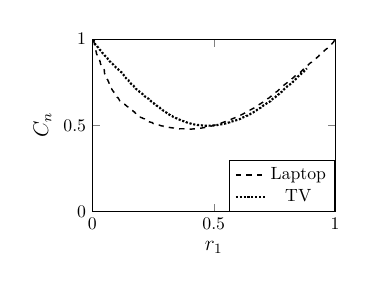
\begin{tikzpicture}[scale=0.64]
\begin{axis}[height=5cm,
width=6.4cm,
xmin=0,
xmax=1,
ymin=0,
ymax=1,legend style={at={(1,0)},anchor=south east},xlabel=$r_1$, ylabel=$C_n$,ylabel near ticks, xtick={0, 0.5, 1}, ytick={0, 0.5, 1}, label style={font=\large}, tick style={font=\Large}
]
\addplot+ [color=black,mark=none,dashed,thick] coordinates
{(0.00406504065041,0.994927984813)(0.00452488687783,0.993463031445)(0.00529100529101,0.991695538904)(0.00555555555556,0.989424703892)(0.00625,0.987734771574)(0.0062893081761,0.986693484021)(0.00641025641026,0.985572042171)(0.00645161290323,0.984529228754)(0.00655737704918,0.983423483399)(0.00662251655629,0.982357884829)(0.00724637681159,0.980747443537)(0.008,0.97901319797)(0.00833333333333,0.973697123519)(0.00840336134454,0.97163332338)(0.00847457627119,0.970566979265)(0.00892857142857,0.96913524293)(0.00896860986547,0.968099974961)(0.00990099009901,0.965220887571)(0.01,0.96214213198)(0.010101010101,0.95806798954)(0.0102040816327,0.956977105563)(0.010752688172,0.95547186289)(0.010989010989,0.954258939031)(0.0111731843575,0.953095312367)(0.0113636363636,0.951926626673)(0.0114285714286,0.950874546773)(0.0119047619048,0.949444041576)(0.0125,0.944936548223)(0.0126582278481,0.943802608752)(0.012987012987,0.942514338453)(0.0130718954248,0.941448525265)(0.0142857142857,0.935416968818)(0.0144927536232,0.934245567572)(0.0147058823529,0.93208420424)(0.015,0.930837563452)(0.0151515151515,0.929718504845)(0.0152284263959,0.928666031075)(0.016393442623,0.926653906965)(0.0165289256198,0.92555271217)(0.0166666666667,0.918561759729)(0.0172413793103,0.917083843865)(0.0173913043478,0.915974398588)(0.0176991150442,0.914729796505)(0.0181818181818,0.913336409783)(0.01875,0.911871827411)(0.0196078431373,0.909186821937)(0.02,0.906903553299)(0.0204081632653,0.904609965814)(0.0207373271889,0.903359142904)(0.0208768267223,0.902268897767)(0.0217391304348,0.900573824763)(0.0228310502283,0.898690401687)(0.0238095238095,0.89690597051)(0.0245901639344,0.895290005825)(0.025,0.892055837563)(0.0252100840336,0.890918397816)(0.0253807106599,0.889814218351)(0.0254237288136,0.888815280048)(0.025641025641,0.887674085644)(0.0262008733624,0.886254516437)(0.0267857142857,0.884816896302)(0.0285714285714,0.882407541697)(0.0288461538462,0.881228035923)(0.0299145299145,0.878454596729)(0.03,0.877431472081)(0.0301507537688,0.876356401296)(0.0302375809935,0.875333019044)(0.030303030303,0.874327026611)(0.0304568527919,0.873251050014)(0.031914893617,0.871141591965)(0.0322580645161,0.868970034387)(0.0333333333333,0.859593908629)(0.0338983050847,0.858212165534)(0.0344827586207,0.854927358656)(0.0357142857143,0.853045685279)(0.0375,0.84980964467)(0.0388888888889,0.847822899041)(0.0389016018307,0.84687706908)(0.0395480225989,0.845455849035)(0.04,0.844182741117)(0.0407523510972,0.842687331922)(0.0409836065574,0.84158275776)(0.0413223140496,0.840399379116)(0.0416666666667,0.836421319797)(0.0428571428571,0.83461928934)(0.0442477876106,0.832675980414)(0.0443037974684,0.831709824584)(0.0444444444444,0.830682459109)(0.0447368421053,0.829545818862)(0.045197740113,0.828288737847)(0.0454545454545,0.827180433779)(0.0461538461538,0.825755564233)(0.0481927710843,0.823374717143)(0.0490196078431,0.821867224047)(0.0493827160494,0.82069311274)(0.0494949494949,0.819698507922)(0.0496894409938,0.818646151906)(0.05,0.804720812183)(0.0502283105023,0.803652968037)(0.0503597122302,0.801738304788)(0.0507246376812,0.80058118149)(0.0508474576271,0.799587025725)(0.0520231213873,0.797893254306)(0.0526315789474,0.796580283195)(0.0527859237537,0.795569912321)(0.0529411764706,0.794559570021)(0.0545454545455,0.792598061837)(0.0552763819095,0.790311965921)(0.0558659217877,0.789025323994)(0.056,0.788036548223)(0.0561797752809,0.787018764615)(0.05625,0.786072335025)(0.0566037735849,0.784943970884)(0.0569105691057,0.783847137964)(0.0572390572391,0.782737698474)(0.0582524271845,0.781193632645)(0.0583333333333,0.77934856176)(0.0585774058577,0.778297899454)(0.0588235294118,0.775455359809)(0.0594059405941,0.773302507916)(0.0595238095238,0.772335025381)(0.0599078341014,0.771204004772)(0.06,0.769360406091)(0.0604026845638,0.76822130617)(0.0617283950617,0.766522529297)(0.0632318501171,0.764721406579)(0.0632911392405,0.763798753454)(0.0635838150289,0.762735835216)(0.0641025641026,0.761538461538)(0.0642857142857,0.760543872371)(0.0644171779141,0.759580828999)(0.0647482014388,0.758499799145)(0.0652173913043,0.757338335908)(0.0666666666667,0.75296108291)(0.0672268907563,0.751755321418)(0.0676056338028,0.750657038679)(0.0683760683761,0.748457633737)(0.0684931506849,0.747514081079)(0.06875,0.745615482234)(0.0688405797101,0.744688442581)(0.0691823899371,0.743619704371)(0.0696202531646,0.742498232988)(0.07,0.740538071066)(0.0701754385965,0.739567192092)(0.0708661417323,0.738310883728)(0.0714285714286,0.736258158086)(0.0716845878136,0.735247348216)(0.0727272727273,0.733807106599)(0.0731707317073,0.732697783831)(0.0733944954128,0.731709588786)(0.0740740740741,0.729610829103)(0.0743405275779,0.728602904478)(0.0745341614907,0.727635022228)(0.0746268656716,0.726721721343)(0.0747663551402,0.725783955596)(0.075,0.720482233503)(0.0756302521008,0.719293605767)(0.0757575757576,0.718366405168)(0.0772727272727,0.716728195662)(0.0780399274047,0.715478087833)(0.0789473684211,0.714159764894)(0.0791366906475,0.713208925246)(0.0793650793651,0.712239142696)(0.08,0.711065989848)(0.0812324929972,0.70959632584)(0.0813953488372,0.708664856569)(0.0819672131148,0.70583340268)(0.0833333333333,0.703468697124)(0.0840336134454,0.702282131127)(0.0845070422535,0.701208264817)(0.0848214285714,0.700213016679)(0.0849056603774,0.699329566134)(0.0857142857143,0.698100072516)(0.0867579908676,0.696761931252)(0.0869565217391,0.695828735379)(0.0875,0.694733502538)(0.0888030888031,0.693283421202)(0.0888888888889,0.691573604061)(0.09,0.689390862944)(0.090395480226,0.688376494881)(0.0904977375566,0.687497990215)(0.0916666666667,0.685304568528)(0.0925925925926,0.6840571536)(0.09375,0.682709390863)(0.0948275862069,0.680579380361)(0.0958904109589,0.67928516793)(0.0963302752294,0.678270386066)(0.0970873786408,0.677117934059)(0.0971659919028,0.676265439076)(0.0977443609023,0.675195603221)(0.0983606557377,0.674111675127)(0.1,0.669340101523)(0.100529100529,0.668304998254)(0.100917431193,0.667331066921)(0.101265822785,0.666375377498)(0.101694915254,0.665387593564)(0.102040816327,0.663627887703)(0.105263157895,0.66150146941)(0.105555555556,0.660580936266)(0.105769230769,0.65969347911)(0.105882352941,0.658847417139)(0.106796116505,0.657680745158)(0.108333333333,0.655473773266)(0.108860759494,0.654470217824)(0.108910891089,0.6536563301)(0.11,0.650852791878)(0.110169491525,0.649995698185)(0.110552763819,0.649057470092)(0.111111111111,0.647264523407)(0.11170212766,0.646252295064)(0.111731843575,0.645452740833)(0.112244897959,0.64447322076)(0.1125,0.643591370558)(0.115523465704,0.641690337005)(0.116666666667,0.639712351946)(0.117647058824,0.638578680203)(0.118072289157,0.637649073451)(0.118421052632,0.636748597382)(0.118644067797,0.635894347415)(0.119047619048,0.6349770365)(0.119402985075,0.634078339268)(0.12,0.633096446701)(0.120567375887,0.632127299564)(0.123711340206,0.630268459888)(0.125,0.629060913706)(0.126262626263,0.627867507563)(0.128205128205,0.626448002083)(0.13,0.625086294416)(0.132295719844,0.623563570286)(0.133858267717,0.622295055758)(0.134020618557,0.621497723586)(0.135593220339,0.620235739482)(0.135714285714,0.619456127629)(0.136363636364,0.618504845408)(0.136690647482,0.617660592338)(0.1375,0.616662436548)(0.14,0.615126903553)(0.140287769784,0.61430449549)(0.140703517588,0.613442848762)(0.141666666667,0.612411167513)(0.142857142857,0.610587382161)(0.14371257485,0.60959907596)(0.146341463415,0.608072304073)(0.146551724138,0.607290390338)(0.148648648649,0.605940458225)(0.14954954955,0.604957241505)(0.15,0.60269035533)(0.150537634409,0.601823044594)(0.153846153846,0.600156188989)(0.15625,0.598762690355)(0.156862745098,0.597889917388)(0.157142857143,0.597113850616)(0.158415841584,0.596059707494)(0.158536585366,0.595332425405)(0.158878504673,0.594544333223)(0.15923566879,0.593753435287)(0.159663865546,0.592944589003)(0.16,0.592162436548)(0.160714285714,0.59127991298)(0.161779575329,0.590306570242)(0.1625,0.58942893401)(0.163120567376,0.588580480253)(0.163265306122,0.587858696778)(0.163461538462,0.587124170246)(0.166666666667,0.584940778342)(0.168,0.583926903553)(0.16814159292,0.583217285836)(0.168421052632,0.582473951376)(0.17,0.581411167513)(0.170212765957,0.580689059294)(0.170731707317,0.579893524824)(0.170886075949,0.579187817259)(0.174273858921,0.577711312846)(0.175,0.575558375635)(0.175273865415,0.574835362996)(0.175824175824,0.574050315167)(0.176079734219,0.573334232761)(0.176470588235,0.571931919976)(0.17695473251,0.571168348269)(0.177215189873,0.570455567693)(0.179487179487,0.569308863725)(0.18,0.567898477157)(0.180555555556,0.567131979695)(0.182481751825,0.566082478047)(0.183333333333,0.563333333333)(0.18487394958,0.562385360235)(0.185185185185,0.561684527167)(0.185714285714,0.56094271211)(0.186186186186,0.560214021128)(0.186666666667,0.559485617597)(0.1875,0.557423857868)(0.189189189189,0.556482370696)(0.191666666667,0.554780033841)(0.19298245614,0.553922878262)(0.194690265487,0.553003009748)(0.194968553459,0.552335344635)(0.196347031963,0.55148227986)(0.196629213483,0.550818456625)(0.196721311475,0.550187234751)(0.197530864198,0.548824967099)(0.2,0.545989847716)(0.202127659574,0.545058861648)(0.205128205128,0.54400624756)(0.206349206349,0.543227781806)(0.206896551724,0.541956940312)(0.208333333333,0.541159052453)(0.209523809524,0.540401256949)(0.211111111111,0.539593908629)(0.212121212121,0.538870942932)(0.21554770318,0.537830711557)(0.215859030837,0.537212370581)(0.215909090909,0.536628980157)(0.216049382716,0.536034342295)(0.216666666667,0.53538071066)(0.217391304348,0.534716398146)(0.218487394958,0.534010152284)(0.21875,0.532836294416)(0.219653179191,0.531592382853)(0.220338983051,0.530947259744)(0.221518987342,0.530251236908)(0.222222222222,0.529610829103)(0.223300970874,0.528934010152)(0.223463687151,0.528355500099)(0.224137931034,0.527726238404)(0.225,0.52652284264)(0.22641509434,0.525830859113)(0.228070175439,0.525122450797)(0.229508196721,0.524440376134)(0.230769230769,0.523779773526)(0.231707317073,0.523152160456)(0.233009708738,0.522497659061)(0.233333333333,0.52192893401)(0.234375,0.52130393401)(0.235294117647,0.520692744103)(0.237288135593,0.519470016347)(0.240740740741,0.518687723256)(0.241379310345,0.51811657623)(0.242857142857,0.51749093546)(0.243697478992,0.516913364331)(0.246753246753,0.516197508076)(0.246913580247,0.515673372188)(0.247524752475,0.51461024275)(0.25,0.511421319797)(0.251533742331,0.510846750335)(0.256198347107,0.510148089105)(0.256637168142,0.509635685728)(0.257142857143,0.509122552574)(0.258992805755,0.50856370741)(0.259259259259,0.508065425832)(0.260162601626,0.507548182081)(0.261146496815,0.507032235119)(0.263888888889,0.506472081218)(0.264285714286,0.505982596084)(0.264462809917,0.505499853169)(0.267326732673,0.504960546816)(0.268907563025,0.503988397389)(0.272108843537,0.503470423702)(0.27397260274,0.502983102705)(0.274725274725,0.502515758353)(0.275,0.502055837563)(0.275449101796,0.501595793185)(0.276315789474,0.501135452845)(0.277777777778,0.500676818951)(0.278481012658,0.500224892373)(0.279069767442,0.499775705348)(0.280405405405,0.499331183976)(0.281105990783,0.498888862897)(0.282051282051,0.498451125862)(0.283018867925,0.498017431281)(0.283687943262,0.497584332361)(0.287037037037,0.497189321301)(0.287671232877,0.496766566998)(0.291139240506,0.496395296537)(0.291666666667,0.495558375635)(0.292307692308,0.495150331902)(0.292817679558,0.494741565471)(0.293103448276,0.494328723963)(0.295652173913,0.493983668064)(0.296089385475,0.493582508578)(0.296296296296,0.493175408911)(0.296551724138,0.492770873447)(0.297297297297,0.492385786802)(0.298701298701,0.492029797614)(0.3,0.491675126904)(0.307692307692,0.491214369387)(0.307971014493,0.490837195615)(0.308755760369,0.490486327166)(0.312404287902,0.490286922521)(0.3125,0.489530456853)(0.313725490196,0.489220662884)(0.314606741573,0.488895226145)(0.316666666667,0.488646362098)(0.316831683168,0.48828466603)(0.317647058824,0.487966557181)(0.319444444444,0.48771855612)(0.320512820513,0.487426786412)(0.321626617375,0.487142629273)(0.324137931034,0.486966567478)(0.324675324675,0.486650405432)(0.326530612245,0.486439448876)(0.327044025157,0.486128404048)(0.329853862213,0.486008287146)(0.333333333333,0.484940778342)(0.335664335664,0.484817720351)(0.336363636364,0.48455006922)(0.337579617834,0.484335090045)(0.337704918033,0.484017641674)(0.341176470588,0.484037025978)(0.341772151899,0.483775621667)(0.342465753425,0.483526875739)(0.343234323432,0.483288938031)(0.343511450382,0.483000736234)(0.347457627119,0.483119676503)(0.35,0.482791878173)(0.350515463918,0.482547490711)(0.352112676056,0.482433688425)(0.352941176471,0.482233502538)(0.353535353535,0.482007896221)(0.354085603113,0.481779217445)(0.354166666667,0.48149323181)(0.354430379747,0.481231125104)(0.357142857143,0.480710659898)(0.357664233577,0.480492052318)(0.358024691358,0.480253180422)(0.361842105263,0.480503606733)(0.363543788187,0.480466674248)(0.366666666667,0.480642978003)(0.369047619048,0.480722745951)(0.370786516854,0.480716363429)(0.375,0.480837563452)(0.376623376623,0.480835915354)(0.377049180328,0.480652409087)(0.378151260504,0.480578424263)(0.378378378378,0.480367677322)(0.379746835443,0.480344406605)(0.380281690141,0.480188746693)(0.38166047088,0.480176627102)(0.382608695652,0.480097108806)(0.382716049383,0.479639029893)(0.383084577114,0.479465616082)(0.384615384615,0.479500195236)(0.386138613861,0.47953962909)(0.3875,0.479327411168)(0.388059701493,0.479202969922)(0.388235294118,0.479008659301)(0.389830508475,0.47908457369)(0.39,0.478893401015)(0.391666666667,0.47899323181)(0.392670157068,0.478969888644)(0.393162393162,0.478849407783)(0.393258426966,0.478651685393)(0.39375,0.478534263959)(0.395604395604,0.47869693758)(0.397058823529,0.478784711854)(0.397849462366,0.478740243436)(0.4,0.478375634518)(0.400428265525,0.478266068109)(0.401639344262,0.478330698178)(0.403314917127,0.478503519646)(0.40503875969,0.478693975524)(0.405405405405,0.478584167924)(0.405594405594,0.478435270313)(0.40625,0.478394670051)(0.408602150538,0.478751159871)(0.410447761194,0.47899840897)(0.410714285714,0.478879622915)(0.417721518987,0.480370108591)(0.417910447761,0.480248503675)(0.418803418803,0.480298494512)(0.419642857143,0.480339013778)(0.41975308642,0.480203045685)(0.420560747664,0.48024099815)(0.420634920635,0.480098299895)(0.421524663677,0.480162072341)(0.425,0.480583756345)(0.425287356322,0.480506447284)(0.426470588235,0.480665870409)(0.426523297491,0.480530538726)(0.428217821782,0.480833794039)(0.428571428571,0.480783176215)(0.42962962963,0.4809249859)(0.433121019108,0.48173558796)(0.433333333333,0.48152284264)(0.435483870968,0.481987882757)(0.435643564356,0.48190179424)(0.438095238095,0.48246555475)(0.439306358382,0.482685367213)(0.440366972477,0.482866856052)(0.440677966102,0.482835756689)(0.441666666667,0.483003384095)(0.444444444444,0.48358714044)(0.446043165468,0.483949895921)(0.447619047619,0.484312303602)(0.45,0.484822335025)(0.450819672131,0.484971290672)(0.452261306533,0.48531489937)(0.453237410072,0.48542526385)(0.453333333333,0.485360406091)(0.454545454545,0.48564836179)(0.459183673469,0.487029938879)(0.46,0.487208121827)(0.460317460317,0.487229070985)(0.461538461538,0.487543928153)(0.463636363636,0.488149515459)(0.465408805031,0.488656897487)(0.466666666667,0.489001692047)(0.467532467532,0.48922143846)(0.468253968254,0.489396503102)(0.46835443038,0.489301548545)(0.469158878505,0.489510887613)(0.469465648855,0.489553221994)(0.473451327434,0.490862944162)(0.473684210526,0.4908896607)(0.474226804124,0.491025171385)(0.474747474747,0.491155206891)(0.47619047619,0.491563935219)(0.479087452471,0.492547914536)(0.480519480519,0.492979102116)(0.48167539267,0.493358492572)(0.482142857143,0.493491660624)(0.482394366197,0.493547579896)(0.483333333333,0.493824027073)(0.48427672956,0.494141685024)(0.486607142857,0.494982777375)(0.486956521739,0.495087177224)(0.4875,0.495266497462)(0.488888888889,0.495769881557)(0.491620111732,0.496792672206)(0.492537313433,0.497128570346)(0.493150684932,0.497350671024)(0.493617021277,0.497518090507)(0.494382022472,0.497804140763)(0.495726495726,0.498320968372)(0.5,0.5)(0.503267973856,0.501310507282)(0.504201680672,0.501693469266)(0.505263157895,0.502131979695)(0.505555555556,0.502261703328)(0.508196721311,0.503353582425)(0.510791366906,0.504437059489)(0.510948905109,0.50452406536)(0.511111111111,0.504613649182)(0.5125,0.505241116751)(0.514492753623,0.506106084014)(0.516129032258,0.5068282299)(0.518518518519,0.507877420568)(0.519480519481,0.508326191575)(0.52,0.508629441624)(0.521452145215,0.509299559398)(0.522522522523,0.509809301687)(0.525096525097,0.510981322149)(0.525252525253,0.511100856279)(0.525423728814,0.511227738105)(0.526315789474,0.511675126904)(0.527272727273,0.512155053069)(0.527777777778,0.512436548223)(0.53125,0.514054568528)(0.534482758621,0.515578505164)(0.536312849162,0.516479029011)(0.537459283388,0.517075348468)(0.539325842697,0.518006045742)(0.541899441341,0.519269489266)(0.542253521127,0.519518123972)(0.54347826087,0.520172147429)(0.547169811321,0.521980653194)(0.549295774648,0.523071423465)(0.55,0.523502538071)(0.550458715596,0.523820611931)(0.55223880597,0.524767027805)(0.552631578947,0.525060112209)(0.555555555556,0.526565143824)(0.556818181818,0.527284263959)(0.556962025316,0.52746899698)(0.557692307692,0.527938305349)(0.565789473684,0.5319930537)(0.566666666667,0.53255499154)(0.568888888889,0.533780033841)(0.568965517241,0.533957640469)(0.571428571429,0.535460478608)(0.573099415205,0.536438388696)(0.575757575758,0.537917243501)(0.577968526466,0.539182152894)(0.578571428571,0.539644670051)(0.578947368421,0.539994656692)(0.583333333333,0.542385786802)(0.588888888889,0.545391990976)(0.590909090909,0.546608214121)(0.591666666667,0.547182741117)(0.593406593407,0.548267975679)(0.59477124183,0.549165588401)(0.595505617978,0.549740489363)(0.596153846154,0.55027333073)(0.6,0.552487309645)(0.601694915254,0.553789899338)(0.601895734597,0.55410301441)(0.602510460251,0.554637554956)(0.602941176471,0.555076142132)(0.607142857143,0.557541696882)(0.611764705882,0.560250821141)(0.612068965517,0.560642394539)(0.613333333333,0.561556683587)(0.613445378151,0.561847886363)(0.617647058824,0.564377426097)(0.618421052632,0.565041410633)(0.620689655172,0.566532469806)(0.622222222222,0.567873660462)(0.623376623377,0.568765244907)(0.624338624339,0.569553890366)(0.625,0.570177664975)(0.626373626374,0.571205444302)(0.628865979381,0.572871421843)(0.629213483146,0.57333029145)(0.629310344828,0.57364782076)(0.630769230769,0.574744240531)(0.633928571429,0.576821972444)(0.637037037037,0.578883248731)(0.637931034483,0.579957990548)(0.638157894737,0.580370024045)(0.638888888889,0.581077270164)(0.640909090909,0.582542685741)(0.641666666667,0.583561759729)(0.642857142857,0.585134155185)(0.65243902439,0.591153893772)(0.653846153846,0.592307692308)(0.656862745098,0.594436150095)(0.658333333333,0.595642978003)(0.661016949153,0.597590983395)(0.661290322581,0.598084165711)(0.665573770492,0.60102521428)(0.669565217391,0.603804899581)(0.670454545455,0.604695431472)(0.671232876712,0.605521173771)(0.672727272727,0.606792801108)(0.673076923077,0.607360406091)(0.673913043478,0.608585301258)(0.675,0.60961928934)(0.675126903553,0.610054368832)(0.676258992806,0.611123689881)(0.676470588235,0.611615407584)(0.677777777778,0.612803158488)(0.679245283019,0.61409826645)(0.679487179487,0.61461668619)(0.683544303797,0.617952836857)(0.684848484848,0.61916628211)(0.686868686869,0.620848074655)(0.6875,0.621637055838)(0.688559322034,0.62270713241)(0.692307692308,0.625536899649)(0.693693693694,0.626834956784)(0.694362017804,0.62766723403)(0.695652173913,0.628911939969)(0.697674418605,0.630645732499)(0.698412698413,0.631536540166)(0.702702702703,0.634792152559)(0.704347826087,0.636301037299)(0.705882352941,0.638160644969)(0.70625,0.638826142132)(0.706896551724,0.640101522843)(0.710526315789,0.642986908897)(0.7109375,0.643694479695)(0.711627906977,0.644594498879)(0.716666666667,0.64847715736)(0.71875,0.650348984772)(0.719101123596,0.651035190783)(0.72,0.652101522843)(0.720048899756,0.65258213049)(0.721518987342,0.654051275461)(0.721649484536,0.654592077032)(0.72197309417,0.655268489222)(0.729323308271,0.660875539102)(0.729411764706,0.661403404001)(0.73,0.662284263959)(0.730769230769,0.663295587661)(0.731958762887,0.664608299754)(0.733333333333,0.667005076142)(0.734693877551,0.668455402466)(0.737373737374,0.670860893196)(0.7375,0.671434010152)(0.73786407767,0.672179784141)(0.738853503185,0.673380969317)(0.738888888889,0.673891708968)(0.74,0.675187817259)(0.740088105727,0.675739618507)(0.740740740741,0.677194961459)(0.741379310345,0.678155084894)(0.741935483871,0.679056820043)(0.744075829384,0.681136478456)(0.744985673352,0.682309135601)(0.745762711864,0.683386389056)(0.75,0.687563451777)(0.752293577982,0.689796488614)(0.755905511811,0.693033294696)(0.760330578512,0.696899777657)(0.763888888889,0.700662718556)(0.764227642276,0.701456811522)(0.764705882353,0.702358913108)(0.766233766234,0.704067506098)(0.767676767677,0.705717069169)(0.768115942029,0.706598984772)(0.769230769231,0.70800468567)(0.770053475936,0.709188631613)(0.770491803279,0.710077390364)(0.771428571429,0.711356055112)(0.771739130435,0.712149635842)(0.772727272727,0.713474850023)(0.774509803922,0.715427490793)(0.774647887324,0.716093515407)(0.776859504132,0.71839577128)(0.778571428571,0.72031182016)(0.778947368421,0.721175527652)(0.779220779221,0.721959259015)(0.78064516129,0.723661372196)(0.781094527363,0.724590246736)(0.784615384615,0.727981257321)(0.785123966942,0.728967571423)(0.7875,0.732043147208)(0.790322580645,0.734910758146)(0.790909090909,0.735976003692)(0.791139240506,0.736753839234)(0.797297297297,0.742365207847)(0.798319327731,0.743804120633)(0.8,0.74578680203)(0.803418803419,0.749203870016)(0.807142857143,0.752886149384)(0.808333333333,0.754492385787)(0.8125,0.758565989848)(0.816091954023,0.762179823794)(0.816455696203,0.763124076335)(0.818181818182,0.765205353023)(0.819047619048,0.766574812666)(0.821229050279,0.769049712163)(0.821428571429,0.769869470631)(0.825,0.773527918782)(0.825396825397,0.774522600919)(0.828571428571,0.777868020305)(0.83,0.779746192893)(0.830508474576,0.781519401187)(0.831683168317,0.783193446248)(0.833333333333,0.785279187817)(0.84,0.791675126904)(0.843137254902,0.795063202946)(0.848101265823,0.800038552978)(0.851239669421,0.80345681084)(0.857142857143,0.80928208847)(0.858974358974,0.811597032409)(0.860759493671,0.813879072158)(0.860869565217,0.814707570073)(0.862385321101,0.816765240069)(0.864864864865,0.819673480587)(0.865979381443,0.821393060861)(0.866666666667,0.822741116751)(0.869318181818,0.825824873096)(0.870229007634,0.827380168171)(0.871794871795,0.82951971886)(0.873873873874,0.832121461563)(0.875,0.833883248731)(0.876712328767,0.836172727905)(0.881355932203,0.841090940377)(0.882352941176,0.843535383697)(0.888172043011,0.849551880356)(0.89,0.851989847716)(0.890410958904,0.853153466379)(0.892307692308,0.855665755564)(0.896551724138,0.861123752844)(0.903225806452,0.868020304569)(0.903703703704,0.869276179733)(0.90780141844,0.873852467869)(0.911764705882,0.87832188713)(0.918367346939,0.885237749922)(0.92,0.887593908629)(0.92380952381,0.891970026589)(0.924369747899,0.893349827241)(0.929411764706,0.898895192595)(0.932989690722,0.903098016641)(0.933333333333,0.906057529611)(0.936507936508,0.909918620579)(0.938775510204,0.9129389827)(0.942857142857,0.917679477883)(0.946666666667,0.922179357022)(0.950819672131,0.927020054922)(0.954545454545,0.931472081218)(0.955223880597,0.933040381847)(0.955555555556,0.934280879865)(0.958333333333,0.937859560068)(0.97037037037,0.950313968791)(0.974489795918,0.955221174764)(0.979797979798,0.961288006973)(0.981818181818,0.964208583295)(0.983050847458,0.967357825002)(0.985,0.970228426396)(0.985714285714,0.971907179115)(0.986666666667,0.973820642978)(0.988888888889,0.976976875353)(0.990476190476,0.979521392313)(0.992481203008,0.982481584672)(1.0,1.0)};
\addplot+ [color=black,mark=none,densely dotted, very thick] coordinates
{(0.0026455026455,0.996355793545)(0.00625,0.991767068273)(0.00632911392405,0.990696965075)(0.00714285714286,0.988898450947)(0.00746268656716,0.987592159684)(0.0077519379845,0.986317362473)(0.00833333333333,0.983768406961)(0.00862068965517,0.982498961363)(0.00952380952381,0.980627270989)(0.00980392156863,0.979368454209)(0.01,0.978192771084)(0.0104166666667,0.976803045515)(0.0105263157895,0.975713379835)(0.010752688172,0.974510947014)(0.0125,0.970858433735)(0.012987012987,0.969410107964)(0.0167597765363,0.964803347468)(0.0168067226891,0.963787924808)(0.02,0.959759036145)(0.0201005025126,0.95869911808)(0.0214285714286,0.956468732071)(0.0215053763441,0.955434641793)(0.0246153846154,0.951519925857)(0.025,0.950200803213)(0.0280373831776,0.945426566077)(0.0289855072464,0.943585937955)(0.029702970297,0.941965883335)(0.0298507462687,0.940882934724)(0.0314465408805,0.938445606325)(0.0367647058824,0.932538979447)(0.037037037037,0.931355049829)(0.0377358490566,0.9297757066)(0.0388888888889,0.926851851852)(0.04,0.923975903614)(0.0404858299595,0.922605401363)(0.041958041958,0.920331676356)(0.0446428571429,0.916953528399)(0.0479704797048,0.912998858904)(0.0487804878049,0.911352727985)(0.05,0.90843373494)(0.0503597122302,0.907204356996)(0.0512820512821,0.90546802595)(0.0526315789474,0.903350243078)(0.0596330275229,0.896153421024)(0.06,0.894939759036)(0.0612244897959,0.892959593476)(0.0620689655172,0.891323916355)(0.0625,0.888303212851)(0.0632911392405,0.886724111636)(0.0647482014388,0.884559822022)(0.0666666666667,0.881994645248)(0.0673076923077,0.8796918443)(0.0677966101695,0.878394935675)(0.0689655172414,0.875640493007)(0.0697674418605,0.874077706174)(0.0714285714286,0.871772805508)(0.075,0.867821285141)(0.0756302521008,0.865571529817)(0.077380952381,0.863214763817)(0.0833333333333,0.857262382865)(0.0838323353293,0.855998845682)(0.0849056603774,0.854247177389)(0.0864197530864,0.852124547573)(0.0869565217391,0.850838135149)(0.0875,0.849548192771)(0.0886075949367,0.84778353922)(0.090395480226,0.84544959499)(0.0918727915194,0.843384137256)(0.0958904109589,0.839192385982)(0.0962962962963,0.838041053101)(0.0967741935484,0.836831195751)(0.0987654320988,0.834362139918)(0.100840336134,0.831831527792)(0.104545454545,0.82795728368)(0.106666666667,0.825408299866)(0.107692307692,0.822984244671)(0.108786610879,0.821297743274)(0.109243697479,0.820137693632)(0.110599078341,0.818245331557)(0.114035087719,0.814662157402)(0.114285714286,0.813683304647)(0.120689655172,0.807713613073)(0.123028391167,0.805059354136)(0.125,0.801204819277)(0.125925925926,0.799709950915)(0.125984251969,0.79891218417)(0.126050420168,0.798108399987)(0.127118644068,0.796508066163)(0.127659574468,0.795330257199)(0.127777777778,0.794489067381)(0.129032258065,0.792751651768)(0.13,0.79124497992)(0.130081300813,0.790438175466)(0.130434782609,0.78941854374)(0.13125,0.788039658635)(0.131926121372,0.786772419493)(0.132075471698,0.785917253921)(0.132275132275,0.785023692654)(0.132352941176,0.784225135837)(0.132530120482,0.783350268544)(0.132653061224,0.782517826408)(0.133333333333,0.780522088353)(0.136531365314,0.77734554454)(0.1375,0.775878514056)(0.138461538462,0.774420759963)(0.139240506329,0.773105078542)(0.140350877193,0.771542309589)(0.141509433962,0.76994771539)(0.145251396648,0.766417625811)(0.148148148148,0.763535623977)(0.148846960168,0.762307089995)(0.149171270718,0.761360358561)(0.14953271028,0.760387343768)(0.149758454106,0.759516326174)(0.15,0.756526104418)(0.150943396226,0.755133742517)(0.151724137931,0.753863730785)(0.152671755725,0.752475551059)(0.152727272727,0.751737860533)(0.154545454545,0.749726177437)(0.154929577465,0.748062673228)(0.156462585034,0.746270797476)(0.156976744186,0.745213411787)(0.157894736842,0.743870217713)(0.158333333333,0.742871485944)(0.16,0.741004016064)(0.164285714286,0.737292025244)(0.166666666667,0.734270414993)(0.167597765363,0.732948553993)(0.169491525424,0.730957729222)(0.169724770642,0.730131535316)(0.169811320755,0.729408198833)(0.17,0.728614457831)(0.171428571429,0.726965002869)(0.171717171717,0.726106445986)(0.172222222222,0.725100401606)(0.172727272727,0.724096385542)(0.173267326733,0.723070499821)(0.174603174603,0.721505067891)(0.175438596491,0.720284647361)(0.176100628931,0.719184915764)(0.176470588235,0.718284904323)(0.177215189873,0.717134360226)(0.178294573643,0.715762273902)(0.178571428571,0.714285714286)(0.179166666667,0.713244645248)(0.181818181818,0.710843373494)(0.182389937107,0.709826728297)(0.182608695652,0.709044875153)(0.18487394958,0.706920117445)(0.186274509804,0.705370501614)(0.1875,0.703313253012)(0.189189189189,0.701590144361)(0.189873417722,0.700523613441)(0.192307692308,0.698331788693)(0.19298245614,0.697280349468)(0.19387755102,0.696090484387)(0.194117647059,0.695322466336)(0.19512195122,0.694068958762)(0.197674418605,0.691837115905)(0.2,0.689759036145)(0.201680672269,0.688096925517)(0.20297029703,0.686687343433)(0.203883495146,0.685518774126)(0.204301075269,0.684663384722)(0.204819277108,0.683747036338)(0.205607476636,0.682665240401)(0.207207207207,0.681084699157)(0.208955223881,0.679419169214)(0.209090909091,0.678751369113)(0.209944751381,0.677644278773)(0.21,0.67702811245)(0.210084033613,0.675812493672)(0.210526315789,0.674963009934)(0.212765957447,0.673032555755)(0.21359223301,0.671959683394)(0.214285714286,0.670969592656)(0.215384615385,0.669740500463)(0.215517241379,0.669090153718)(0.218181818182,0.66694048923)(0.220183486239,0.665192881618)(0.224137931034,0.662304389974)(0.224719101124,0.661409683679)(0.225,0.660692771084)(0.225352112676,0.659935516715)(0.227941176471,0.657881526104)(0.228169014085,0.657203461734)(0.230769230769,0.654618473896)(0.232142857143,0.653291738382)(0.232558139535,0.652517044924)(0.232673267327,0.651914589049)(0.232876712329,0.650726192441)(0.233333333333,0.649397590361)(0.236180904523,0.647272507114)(0.236220472441,0.646720741233)(0.237288135593,0.645599346539)(0.239130434783,0.644054478785)(0.239316239316,0.643428414513)(0.240458015267,0.642279039823)(0.240740740741,0.64160345084)(0.242105263158,0.640340308603)(0.242990654206,0.639342416395)(0.243697478992,0.63844453444)(0.244635193133,0.63742523743)(0.245689655172,0.636347112588)(0.246376811594,0.635469413887)(0.246575342466,0.634854486439)(0.247126436782,0.6340534552)(0.248322147651,0.632914207164)(0.25,0.630522088353)(0.25311942959,0.628397726378)(0.253164556962,0.62787860302)(0.253968253968,0.626968190221)(0.254237288136,0.625842352461)(0.256756756757,0.624063822859)(0.257142857143,0.623379231211)(0.258333333333,0.621803882195)(0.259615384615,0.620675007723)(0.260869565217,0.619565217391)(0.261682242991,0.618680328792)(0.262068965517,0.618009970918)(0.262931034483,0.61710635646)(0.263157894737,0.616518706405)(0.264367816092,0.615450306975)(0.266331658291,0.614018889629)(0.266666666667,0.613386880857)(0.26875,0.611910140562)(0.27027027027,0.610713122761)(0.270833333333,0.609521419009)(0.273273273273,0.607900068743)(0.2734082397,0.607380834198)(0.274509803922,0.606406016222)(0.275,0.605722891566)(0.275641025641,0.604971166718)(0.277108433735,0.603837034887)(0.277372262774,0.60326708293)(0.278481012658,0.601418331554)(0.278846153846,0.600807074452)(0.279279279279,0.600166431492)(0.279569892473,0.599149285313)(0.280104712042,0.598467167098)(0.28025477707,0.597958713836)(0.280701754386,0.597319100965)(0.281481481481,0.596534285289)(0.282051282051,0.595407270106)(0.282828282828,0.59463104945)(0.286764705882,0.592487597449)(0.287878787879,0.591578434952)(0.288288288288,0.590976518687)(0.288888888889,0.590294511379)(0.288939051919,0.589849238942)(0.29,0.588975903614)(0.290398126464,0.588386332214)(0.291666666667,0.586596385542)(0.292763157895,0.585724476855)(0.294117647059,0.584337349398)(0.295774647887,0.583248486905)(0.296875,0.582392068273)(0.29702970297,0.581921746392)(0.297520661157,0.580910418534)(0.297794117647,0.580395109851)(0.298850574713,0.579571158196)(0.3,0.578313253012)(0.301204819277,0.577442299318)(0.301587301587,0.576894881112)(0.303571428571,0.575731497418)(0.305194805195,0.574714442184)(0.306930693069,0.572885601813)(0.307142857143,0.572418244406)(0.307291666667,0.571975401606)(0.309734513274,0.570680953904)(0.31,0.570200803213)(0.310606060606,0.569596568091)(0.310924369748,0.569099929128)(0.311111111111,0.568652387327)(0.3125,0.566641566265)(0.313043478261,0.566072987603)(0.314285714286,0.565261044177)(0.315068493151,0.564614622875)(0.315789473684,0.563253012048)(0.317307692308,0.562364843991)(0.317757009346,0.561845512893)(0.318681318681,0.561167747915)(0.320512820513,0.560189475852)(0.320675105485,0.559774964838)(0.322033898305,0.558607310598)(0.322314049587,0.558158252846)(0.322727272727,0.557667031763)(0.324873096447,0.556617332273)(0.326530612245,0.555384804524)(0.328767123288,0.554326896628)(0.329608938547,0.553717663952)(0.329787234043,0.553319661625)(0.330275229358,0.55282598283)(0.330508474576,0.552413041999)(0.331775700935,0.55168336899)(0.333333333333,0.54953145917)(0.336956521739,0.548127291776)(0.3375,0.547640562249)(0.338129496403,0.547130969923)(0.338235294118,0.546775336641)(0.338461538462,0.546385542169)(0.338888888889,0.545939312807)(0.340611353712,0.545128110696)(0.340659340659,0.544794562867)(0.341365461847,0.544277511653)(0.342465753425,0.543654068328)(0.342723004695,0.543266964572)(0.34375,0.542670682731)(0.345070422535,0.541998981843)(0.34693877551,0.541185148758)(0.347457627119,0.540739228099)(0.349206349206,0.539969401415)(0.35,0.538855421687)(0.350877192982,0.538328753611)(0.352941176471,0.537502952988)(0.353383458647,0.537095751427)(0.353846153846,0.53609823911)(0.354285714286,0.53569707401)(0.354838709677,0.535270112709)(0.355263157895,0.534876347495)(0.35761589404,0.534023511264)(0.357894736842,0.533671528218)(0.36,0.532610441767)(0.361990950226,0.531869559687)(0.36231884058,0.531517373843)(0.363636363636,0.530941949617)(0.364016736402,0.530582581372)(0.365079365079,0.530072671639)(0.365217391304,0.529771258949)(0.365384615385,0.529193697868)(0.366197183099,0.528748798009)(0.366666666667,0.528380187416)(0.368421052632,0.527742549144)(0.368852459016,0.527388241491)(0.369369369369,0.527017981837)(0.371794871795,0.526258881681)(0.372093023256,0.525940973195)(0.373134328358,0.525475034466)(0.374613003096,0.52492633071)(0.375,0.524598393574)(0.376712328767,0.524013863674)(0.377192982456,0.523673641936)(0.377358490566,0.523395468667)(0.378378378378,0.522956691631)(0.379310344828,0.52253842958)(0.379746835443,0.522215444055)(0.380281690141,0.521876237344)(0.380952380952,0.521514629948)(0.381679389313,0.52090805972)(0.384615384615,0.52015755329)(0.385,0.519859437751)(0.385964912281,0.519234834073)(0.386075949367,0.518987341772)(0.3875,0.518298192771)(0.388059701493,0.51798237727)(0.388461538462,0.517693852332)(0.389473684211,0.517089410273)(0.390476190476,0.516714476955)(0.392405063291,0.516204056733)(0.392857142857,0.515920826162)(0.39378238342,0.51557005223)(0.394736842105,0.515218769816)(0.394957983193,0.514975869866)(0.395833333333,0.514641900937)(0.396551724138,0.514333194848)(0.396825396825,0.514088098425)(0.397058823529,0.51384951571)(0.398305084746,0.513477639371)(0.4,0.511847389558)(0.402985074627,0.511298927051)(0.404761904762,0.510900745841)(0.405405405405,0.510637143167)(0.405660377358,0.510419034629)(0.40625,0.510165662651)(0.407142857143,0.50988238669)(0.407407407407,0.509668302841)(0.407894736842,0.509432466709)(0.408284023669,0.509208431359)(0.409090909091,0.508762322015)(0.41,0.508493975904)(0.410071942446,0.508306607726)(0.410526315789,0.508084971465)(0.410714285714,0.507888697648)(0.411657559199,0.507627961756)(0.411764705882,0.507264351524)(0.412280701754,0.507045726767)(0.4125,0.506852409639)(0.413461538462,0.506603336423)(0.416666666667,0.506191432396)(0.41726618705,0.505980757563)(0.421232876712,0.505535841998)(0.421428571429,0.5053643144)(0.421686746988,0.505189432429)(0.423333333333,0.504926372155)(0.425,0.504518072289)(0.425925925926,0.504313550498)(0.427272727273,0.504089083607)(0.428571428571,0.503729202524)(0.428909952607,0.50356877748)(0.43,0.503373493976)(0.431034482759,0.503185154411)(0.431279620853,0.503035840043)(0.431818181818,0.50273822563)(0.432258064516,0.502584531675)(0.434782608696,0.502357255107)(0.4375,0.502133534137)(0.440476190476,0.501792885829)(0.440677966102,0.5016676877)(0.441666666667,0.501522757697)(0.442477876106,0.501270569002)(0.443037974684,0.501143815769)(0.444444444444,0.501004016064)(0.44502617801,0.500883113606)(0.445454545455,0.500766703176)(0.448275862069,0.500623182385)(0.449275362319,0.500509283511)(0.45,0.500401606426)(0.450704225352,0.500296962498)(0.451923076923,0.500193080012)(0.452261306533,0.50009586083)(0.452991452991,0.5)(0.453488372093,0.499813206314)(0.453703703704,0.499721106649)(0.453781512605,0.49962876717)(0.454545454545,0.499361080686)(0.454901960784,0.499275533507)(0.45652173913,0.499214248298)(0.457627118644,0.499149138929)(0.458181818182,0.499076305221)(0.458333333333,0.498995983936)(0.458823529412,0.498925112214)(0.459016393443,0.498847850418)(0.459459459459,0.498778899381)(0.46,0.498714859438)(0.460869565217,0.498664222106)(0.461538461538,0.498455359901)(0.462264150943,0.498408729257)(0.463541666667,0.498389390897)(0.464751958225,0.498372078392)(0.465517241379,0.498338180307)(0.466666666667,0.498326639893)(0.467105263158,0.498282604101)(0.469135802469,0.498326639893)(0.469387755102,0.498278829604)(0.469565217391,0.498227693382)(0.470085470085,0.498197919885)(0.474576271186,0.498366346743)(0.474820143885,0.498331455318)(0.475935828877,0.498357064622)(0.476744186047,0.498365555244)(0.476821192053,0.498324423522)(0.478260869565,0.498384843723)(0.478723404255,0.498376484662)(0.48,0.49843373494)(0.481481481481,0.498512568794)(0.481751824818,0.498497640196)(0.482412060302,0.498516679784)(0.483333333333,0.498527443106)(0.484848484848,0.498630887185)(0.485106382979,0.498624284372)(0.485714285714,0.498651749857)(0.486111111111,0.498661311914)(0.486486486486,0.498643221535)(0.486725663717,0.498640580019)(0.486842105263,0.49862608328)(0.487179487179,0.498635567913)(0.487394957983,0.498633188215)(0.487804878049,0.498653149182)(0.489208633094,0.498786512958)(0.49,0.498855421687)(0.490909090909,0.498941219423)(0.491525423729,0.498995983936)(0.491666666667,0.498995983936)(0.492307692308,0.49905776954)(0.495652173913,0.499458704383)(0.496732026144,0.499586581621)(0.5,0.5)(0.503649635036,0.500513000909)(0.504545454545,0.500648046732)(0.504854368932,0.500701836472)(0.505882352941,0.50086227262)(0.506172839506,0.500917249244)(0.507772020725,0.501170485049)(0.508771929825,0.501338688086)(0.509433962264,0.501458664848)(0.51,0.50156626506)(0.510101010101,0.501602369072)(0.510752688172,0.501727339465)(0.511111111111,0.501807228916)(0.512820512821,0.502111008135)(0.513513513514,0.502252252252)(0.516245487365,0.502740202688)(0.516666666667,0.502844712182)(0.517985611511,0.503105948976)(0.518518518519,0.503272348654)(0.520491803279,0.503662189743)(0.521739130435,0.503928758512)(0.523510971787,0.504296181592)(0.525,0.504618473896)(0.525641025641,0.504788384306)(0.526315789474,0.505072923272)(0.526717557252,0.505204022196)(0.52688172043,0.505289977113)(0.527777777778,0.505522088353)(0.528301886792,0.505683109798)(0.528409090909,0.505761683096)(0.533333333333,0.506894243641)(0.537558685446,0.507843580896)(0.537634408602,0.507934965669)(0.540540540541,0.508710517747)(0.540816326531,0.508851733464)(0.541176470588,0.509012520671)(0.54128440367,0.509119044987)(0.542857142857,0.509552495697)(0.544554455446,0.510020279136)(0.544642857143,0.510129804934)(0.545762711864,0.510475801511)(0.546153846154,0.510658016682)(0.54748603352,0.511061003792)(0.548387096774,0.511368052857)(0.55,0.512048192771)(0.550387596899,0.512242769528)(0.550847457627,0.512456606085)(0.551181102362,0.512641115644)(0.551724137931,0.512879102617)(0.552631578947,0.513210737688)(0.553191489362,0.51345808767)(0.554347826087,0.513859786974)(0.555555555556,0.514279339581)(0.557692307692,0.515060240964)(0.557971014493,0.515249403411)(0.56,0.515903614458)(0.561403508772,0.516522229268)(0.562091503268,0.516832034018)(0.562582345191,0.517090760936)(0.56338028169,0.517435940947)(0.564935064935,0.517994054139)(0.565610859729,0.51831307129)(0.565656565657,0.51845766906)(0.566666666667,0.518875502008)(0.566878980892,0.519069910214)(0.567164179104,0.519286099622)(0.56880733945,0.519896098154)(0.569230769231,0.520296570899)(0.569620253165,0.520550556657)(0.569721115538,0.520720331525)(0.570776255708,0.521176028314)(0.57264957265,0.5218824014)(0.573221757322,0.522201777823)(0.575,0.522891566265)(0.576811594203,0.523598742797)(0.577586206897,0.523992521811)(0.578313253012,0.524374606861)(0.58,0.525060240964)(0.586826347305,0.527372964914)(0.586956521739,0.527588615331)(0.5875,0.527936746988)(0.588235294118,0.528348688873)(0.591836734694,0.529690189329)(0.593073593074,0.530276951964)(0.593220338983,0.530511878021)(0.594202898551,0.53102264129)(0.598326359833,0.532578010788)(0.6,0.533534136546)(0.600938967136,0.534051699757)(0.601694915254,0.534510925056)(0.605042016807,0.535857716581)(0.605263157895,0.536144578313)(0.605633802817,0.536483964025)(0.606741573034,0.537080907901)(0.608333333333,0.537851405622)(0.610169491525,0.538714178749)(0.611111111111,0.539268183846)(0.611650485437,0.53968300386)(0.612068965517,0.540056778839)(0.6125,0.540436746988)(0.613445378151,0.541004353549)(0.613861386139,0.541383355203)(0.61581920904,0.542327502099)(0.616071428571,0.54288582903)(0.616161616162,0.54315240761)(0.616666666667,0.543808567604)(0.617283950617,0.544275868908)(0.619047619048,0.545180722892)(0.62,0.546024096386)(0.620253164557,0.546362665853)(0.621621621622,0.547378704005)(0.625,0.549196787149)(0.626865671642,0.550185817898)(0.627118644068,0.550541147641)(0.63025210084,0.552048530255)(0.632653061224,0.553274321777)(0.633333333333,0.554350736278)(0.6375,0.556325301205)(0.638554216867,0.557035370397)(0.638888888889,0.557452030344)(0.64,0.558192771084)(0.640449438202,0.558943639727)(0.642857142857,0.560527825588)(0.64406779661,0.561619358791)(0.646739130435,0.563056574123)(0.647975077882,0.56388482278)(0.649122807018,0.564679771718)(0.649350649351,0.565078495801)(0.650793650794,0.566010072034)(0.651041666667,0.566421937751)(0.651685393258,0.56700961148)(0.652173913043,0.567530993539)(0.653465346535,0.568412262913)(0.653846153846,0.568890948409)(0.657142857143,0.570682730924)(0.657303370787,0.571070800054)(0.657342657343,0.571404499115)(0.657777777778,0.571918786256)(0.659192825112,0.5728834621)(0.66,0.573574297189)(0.660377358491,0.574069864363)(0.661764705882,0.575035435861)(0.663636363636,0.576232201533)(0.664912280702,0.577157753822)(0.666666666667,0.578982597055)(0.670212765957,0.581004870546)(0.67032967033,0.58140253321)(0.672413793103,0.582744772192)(0.672727272727,0.583242059146)(0.673076923077,0.584105653383)(0.673469387755,0.584644701254)(0.674242424242,0.585371790191)(0.675,0.58609437751)(0.675438596491,0.586662439231)(0.676136363636,0.587360806864)(0.676300578035,0.587796271792)(0.676691729323,0.588345864662)(0.677685950413,0.589199774304)(0.679245283019,0.591062362658)(0.68152866242,0.592586908142)(0.683333333333,0.593875502008)(0.683760683761,0.594463323379)(0.684210526316,0.5950644684)(0.684563758389,0.595617368804)(0.684931506849,0.596179237498)(0.685393258427,0.596791661026)(0.685534591195,0.597238008638)(0.686666666667,0.598206157965)(0.689655172414,0.6005400914)(0.691666666667,0.601991298527)(0.69387755102,0.603557085485)(0.694117647059,0.604464918498)(0.694610778443,0.605121083135)(0.695652173913,0.606076479832)(0.696428571429,0.606891853127)(0.696721311475,0.607446178155)(0.697478991597,0.608256555634)(0.697530864198,0.608681640141)(0.7,0.61124497992)(0.701754385965,0.612625942366)(0.703125,0.613798945783)(0.703703703704,0.614941246467)(0.704918032787,0.616037922181)(0.705882352941,0.61699740137)(0.708154506438,0.618706586001)(0.711340206186,0.620947708359)(0.712121212121,0.621820615797)(0.712328767123,0.622366177037)(0.713375796178,0.623398050802)(0.716049382716,0.625811889533)(0.716666666667,0.626606425703)(0.718309859155,0.628004977657)(0.71921182266,0.628974024176)(0.720338983051,0.630079640596)(0.722772277228,0.631963497555)(0.723214285714,0.632673551348)(0.725490196078,0.634479092842)(0.728813559322,0.63692056361)(0.730769230769,0.638554216867)(0.732026143791,0.639774785416)(0.73381294964,0.641320678397)(0.733944954128,0.641870233226)(0.73417721519,0.642481317676)(0.734234234234,0.642986359854)(0.734256926952,0.643470607872)(0.734463276836,0.64406779661)(0.735294117647,0.645050791401)(0.735537190083,0.645673603505)(0.735714285714,0.646256454389)(0.735849056604,0.646813669773)(0.738461538462,0.648918751931)(0.74,0.650843373494)(0.740384615385,0.6515678097)(0.741935483871,0.653031480762)(0.743243243243,0.65483555845)(0.745614035088,0.656837877827)(0.746268656716,0.657750404603)(0.747126436782,0.658796103956)(0.75,0.661144578313)(0.752136752137,0.6630281811)(0.753424657534,0.664369807999)(0.755555555556,0.666265060241)(0.756097560976,0.667131942404)(0.75625,0.667745983936)(0.756302521008,0.668295028855)(0.758122743682,0.670008554072)(0.759219088937,0.671251165181)(0.76,0.672289156627)(0.764179104478,0.675588922856)(0.764578833693,0.676385889129)(0.764705882353,0.677002126152)(0.76582278481,0.678282751258)(0.766666666667,0.679384203481)(0.766990291262,0.68013802784)(0.767123287671,0.6807641525)(0.768115942029,0.681974273907)(0.769736842105,0.68361604312)(0.77,0.684337349398)(0.772222222222,0.686401160196)(0.773333333333,0.687710843373)(0.77380952381,0.68858768407)(0.774390243902,0.689538642374)(0.774436090226,0.690121387807)(0.775,0.691064257028)(0.777777777778,0.693551985721)(0.781609195402,0.696787148594)(0.782608695652,0.698053081893)(0.783333333333,0.699129852744)(0.783505154639,0.699819898149)(0.783582089552,0.700443565306)(0.784946236559,0.701979962862)(0.785,0.702590361446)(0.785714285714,0.704245553643)(0.7875,0.706676706827)(0.787610619469,0.707333759818)(0.789473684211,0.709258084971)(0.789915966387,0.710159967601)(0.790909090909,0.71146403797)(0.791666666667,0.712600401606)(0.792307692308,0.713654618474)(0.79347826087,0.715099528549)(0.796610169492,0.717990606494)(0.796875,0.718781375502)(0.8,0.722891566265)(0.801886792453,0.724899598394)(0.802395209581,0.725885578241)(0.803278688525,0.727154519718)(0.803571428571,0.72798336202)(0.807692307692,0.731696014829)(0.808080808081,0.732607196463)(0.81308411215,0.737013474459)(0.813559322034,0.738002858893)(0.816901408451,0.741175971492)(0.821428571429,0.745266781411)(0.823529411765,0.747519489724)(0.824427480916,0.749509488335)(0.824561403509,0.750264214754)(0.825,0.751907630522)(0.827338129496,0.754377221115)(0.830188679245,0.757255436842)(0.831168831169,0.758684086997)(0.833333333333,0.762382864793)(0.835051546392,0.765080942326)(0.83606557377,0.76655803542)(0.8375,0.768373493976)(0.837962962963,0.769420273687)(0.838983050847,0.770914165135)(0.839552238806,0.772050890128)(0.840579710145,0.773558000116)(0.842105263158,0.775470302262)(0.842729970326,0.776661542312)(0.842857142857,0.777452667814)(0.845070422535,0.779936648)(0.845528455285,0.781002057009)(0.845588235294,0.781744625561)(0.847457627119,0.78396637397)(0.847619047619,0.78479632817)(0.85,0.787449799197)(0.85046728972,0.788537326878)(0.852459016393,0.790884850879)(0.855072463768,0.793754729061)(0.858823529412,0.797578549492)(0.859649122807,0.798985415346)(0.860103626943,0.800086355786)(0.867346938776,0.806860093435)(0.867647058824,0.807849043232)(0.868421052632,0.809236947791)(0.87,0.811305220884)(0.870689655172,0.812629829663)(0.871428571429,0.813998852553)(0.872093023256,0.815307742598)(0.875816993464,0.819218048665)(0.876288659794,0.820374280628)(0.876787678768,0.821555749953)(0.878787878788,0.824023366192)(0.879166666667,0.825108768407)(0.880341880342,0.826880170254)(0.882352941176,0.829376328845)(0.883333333333,0.830990629183)};
\legend{Laptop, TV}
\end{axis} 
\end{tikzpicture}
}
\vspace{-0.1in}
\caption{$F_n$ and $C_n$ for Laptop and TV when $k=2$\label{fig:laptoptv}}
\end{figure}

\begin{table}[ht]
\vspace{-0.05in}
\centering
\begin{tabular}{|c|c|c|c|}
\hline
   & $k=2$ & $k=3$ & $k=4$ \\
\hline
\texttt{exhaustive} & 31.72 & 21.27 & 16.14\\ \hline
\texttt{quantile} & 31.85 & 21.30 & 16.19\\ \hline
\end{tabular}
\caption{Optimal ARR vs. \texttt{quantile}'s ARR for `TV'\label{tab:opt}}
\vspace{-0.05in}
\end{table}

To answer this question, we need to find out how \texttt{powell} and \texttt{tree} really works. Recall that \texttt{powell} optimizes $C_n(R)$, which is computed from $F_n(r)$ (Equation~\ref{eq:cr}). When $k=2$, that is, $R=(r_1)$, we are able to plot $C_n(R)$ and $F_n(r)$ as a function of $r_1$. We show the two plots in Figure~\ref{fig:laptoptv}. From Figure~\ref{fig:laptoptv} we can see: $F_n$ of TV is very close to linear, and (consequently) $C_n$ of TV is very close to a quadratic function whose minimum point is $r_1=0.5$ (Indeed, by plugging $F_n(r_1) = r_1$ into Equation~\ref{eq:cr} we get $C_n(r_1) = 2r_1^2 - 2r_1 + 1$). For general $k$, the minimum point $R$ found by these algorithms is almost equal to \texttt{quantile} method. In other words, \texttt{quantile} almost reaches the optimal $R$ on training data in terms of $C_n(R)$.

But our final goal is to optimize ARR \emph{on testing data}. Has \texttt{quantile} method also reached the optimal $R$ on testing data in terms of ARR? To find out the true optimal $R$ on testing data, we perform grid search. We exhaustively enumerate $r_j (j=1,\cdots, k-1$) over all candidate values (i.e., $X_{sorted}$ in Algorithm~\ref{algo}); at each point, we evaluate the true ARR on testing data, and return the minimum value we find. Time complexity of this exhaustive search is $O({{n_0}\choose{k-1}})$. When $k>4$, it becomes intractable. We thus only compute the results for $k\leq 4$\footnote{Although it seems we can replace exhaustive search with Powell's method, which is efficient thus can be applied to $k > 4$; notice Powell's method can not guarantee finding global optimal like exhaustive search.} and show them in Table~\ref{tab:opt} (\texttt{exhaustive}), compared with ARR of \texttt{quantile} method. From Table~\ref{tab:opt} we can see that \texttt{quantile} method indeed almost achieves optimal. So it is difficult for \texttt{tree} and \texttt{powell} to outperform \texttt{quantile}. 

\begin{figure}[h]
\centering
\subfloat{
\begin{tikzpicture} [scale=0.9]
\begin{groupplot}[group style={group size= 1 by 2},height=5cm,width=8cm]%[ybar stacked,xtick=\empty,]%ytick=\empty]
\nextgroupplot[ybar,symbolic x coords={2, 3, 4, 5, 6},  ymin=0, ymax=35,ymajorgrids = true,bar width = 4.5,xtick=data]%ytick=\empty]
\addplot[fill=black,draw=black] 
coordinates {(2,31.03)  (3,19.51) (4,14.94) (5,11.79) (6,9.95)};
\addplot[fill=white,draw=black,pattern=dots] 
coordinates {(2,30.91)  (3,19.42) (4,14.85) (5,11.74) (6,10.02)};
\addplot[fill=white,draw=black,pattern=north west lines] coordinates {(2,28.47) (3,17.97) (4,13.55) (5,10.89) (6,9.1)};
\addplot[fill=white] coordinates {(2,28.69) (3,18.14) (4,13.55) (5,10.92) (6,9.18)};
\end{groupplot}
\end{tikzpicture}
}\\
\vspace{-0.1in}
\subfloat{
\begin{tikzpicture} [scale=0.9]
\begin{groupplot}[group style={group size= 1 by 2},height=5cm,width=8cm]%[ybar stacked,xtick=\empty,]%ytick=\empty]
\nextgroupplot[ybar,symbolic x coords={2, 3, 4, 5, 6},legend style={at={(0.5,-0.2)},anchor=north, ymin=0, ymax=35,legend columns=2},  ymajorgrids = true,bar width = 4.5,xtick=data]%ytick=\empty]
\addplot[fill=black,draw=black] 
coordinates {(2,31.63)  (3,21.41) (4,16.18) (5,13.01) (6,10.96)};
\addplot[fill=white,draw=black,pattern=dots] 
coordinates {(2,31.53)  (3,21.39) (4,16.14) (5,13.01) (6,10.9)};
\addplot[fill=white,draw=black,pattern=north west lines] coordinates {(2,30.62) (3,20.84) (4,15.63) (5,12.51) (6,10.54)};
\addplot[fill=white] coordinates {(2,30.8)  (3,20.78) (4,15.87) (5,12.75) (6,10.56)};
\addlegendentry{LDA}
\addlegendentry{LDA+num}
\addlegendentry{LDA+num+q}
\addlegendentry{LDA+num+q+LSA}
\end{groupplot}
\end{tikzpicture}
}

\caption{Compare importance of different feature groups: ARR for $k=2,\cdots, 6$. Above: Laptop; below: TV\label{fig:treefeat}}
\vspace{-0.2in}
\end{figure}

\subsubsection{Comparative Study on Non-smooth Optimization Methods}
\label{sec:nonsmooth}

In this section we conduct comparative study on the performance of different non-smooth optimization methods. We study five non-smooth algorithms. Besides the aforementioned 1) \texttt{powell} and 2) \texttt{nelder-mead}, we also study: 3) \texttt{cg}: conjugate gradient method in non-smooth case; 4) \texttt{bfgs}: second order optimization method in non-smooth case; and
5) \texttt{slsqp}: sequential least square programming. For all the five methods we use the implementation in Python library\footnote{\url{https://docs.scipy.org/doc/scipy/reference/generated/scipy.optimize.minimize.html}}. For each algorithm, we run 5 fold cross validation to tune the error tolerance as well as to find a good starting point. We report the performance of each algorithm in Table~\ref{tab:nonsmooth}. Due to space limit and since our goal is comparative study, results in Table~\ref{tab:nonsmooth} is the average over $k=2,\cdots, 6$. To ensure the statistical significance, we randomly restart each algorithm 50 times and report the average (i.e., each number in Table~\ref{tab:nonsmooth} is averaged over 50$\times$ 5 values). 

From Table~\ref{tab:nonsmooth} we can see that the five algorithms have slightly different performances: \texttt{slsqp} has the best performance in Laptop and \texttt{powell} has the best performance in TV. \texttt{powell} and \texttt{nelder-mead} has the largest time cost, while \texttt{bfgs} is the fasted algorithm among all. This can be explained by the fact that \texttt{bfgs} is a second order method, while \texttt{Powell} and \texttt{nelder-mead} does not leverage the gradient information compared with the other three. 
\begin{table}
\centering
\begin{tabular}{|c|c|c|c|c|c|c|}
\hline
  \multicolumn{2}{|c|}{} & \texttt{powell} & \texttt{bfgs}& \texttt{nelder} & \texttt{cg} &\texttt{slsqp}\\
\hline
\multirow{2}{*}{\specialcell{avg\\ARR}} &L & 17.77 &  17.58 &  17.78 & 17.60  & \textbf{17.50} \\ \cline{2-7}
&T & \textbf{18.70} & 18.76 & 18.74& 19.06 & 18.76\\ \hline\hline
\multirow{2}{*}{time}&L & 0.024 & \textbf{0.007}&0.028 & 0.012&0.027\\ \cline{2-7}
&T & 0.022 &\textbf{0.008}&0.026 &0.009 &0.009\\ \hline
\end{tabular}
\caption{Compare different non-smooth optimization methods: averaged ARR and running time over $k=2,\cdots, 6$.\label{tab:nonsmooth}}
\vspace{-0.1in}
\end{table}

\subsubsection{Comparative Study on Regression Tree Features}

Since regression tree method (Section~\ref{sec:tree}) uses feature $\mathbf{x}^i$ for each query $q^i$, in this section, we study the influence from different features. We use three groups of features:

\textbf{Semantic representation for $q^i$}: we use both latent semantic analysis (LSA) and latent Dirichlet allocation (LDA). For each method the dimension is set to 20. 

%In order to leverage more co-occurences, both method are run on the mixture of three categories instead of running on each category separately;

\textbf{Number of explicitly mentioned facets in $q^i$}: we use Stanford Named Entity Recognizer (NER) to label the explicitly mentioned facets in each query. For example, for query `17 in refurbished laptop', explicitly mentioned facets are screen size=17 and condition=refurbished, so this feature = 2. We manually label 40\% of the queries for training, the rest are computed by the recognizer. Intuition behind this feature is when user mentions more facets, it is more likely she is looking for a higher profiled product;

\textbf{Quartile absolute values of numerical facets in $E^i$}: we use quartile facets, which are absolute values of the 25\%, 50\% and 75\%th smallest facets in $E^i$. Intuition behind this feature is when retrieved products are all very expensive, user may prefer relatively less expensive products in the list;

 We study four combinations of these features\footnote{In this experiment the splitting criterion of regression tree is fixed to criterion 2 and non-smooth optimization method is fixed to Powell's method. }: (1) LDA (dimension=20): using only 20 features from LDA; (2) LDA + num (dimension=21): adding the number of explicitly mentioned facets; (3) LDA + num + q (dimension=24): \allowbreak adding the quartile absolute value features; (4) LDA + num + q + LSA (dimension=44): adding 20 features from LSA. The comparative results of the four groups is shown in Figure~\ref{fig:treefeat}. Figure~\ref{fig:treefeat} shows that quartile absolute value features is most helpful in reducing ARR; number of explicitly mentioned facets does not help a lot; LSA features also do not help ARR, actually hurts ARR in many cases, which can be explained by the fact that we already have LDA features. 

\subsubsection{Comparative Study on Regression Tree Splitting Criterion}
In Section~\ref{sec:tree}, we discuss the usage of two splitting criteria for building the regression tree. Recall the first criterion is to minimize $C_n(R)$ (Equation~\ref{eq:cr}), while the second criterion is to minimize MSE. Therefore, we denote the first criterion as \texttt{nonsquare} and the second criterion as \texttt{square}. In this section, we study the influence of splitting criterion on the performance of regression tree. In order to make a comprehensive comparison, we look into three trees under each criterion: first, fully grown tree without pruning, denoted as \textsf{full}; second, the smallest tree after pruning, which only contains the root node and two leaf nodes, denoted as \textsf{min}; third, the best ARR among all the pruned trees and the fully grown tree, denoted as \textsf{best} \footnote{In this experiment $\mathbf{x}^i$ is fixed to LDA + num + q and non-smooth optimization method is fixed to Powell's method.}. In Figure~\ref{fig:split} we show $p$ values in the T-test results between the two criteria. When criterion 2 is better, we plot the $p$ value in positive (\texttt{square}); otherwise, we plot the $p$ value in negative (\texttt{nonsquare}). 

From Figure~\ref{fig:split} we can see that the difference between the two criteria are basically consistent over $k=2,\cdots, 6$. Although none of the $p$ values is small enough to show statistical significance, we can still observe a few phenomena: first, \textsf{best} of \texttt{nonsquare} is slightly better than \texttt{square}; second, \textsf{min} of \texttt{nonsquare} is more significantly better than \texttt{square}; third, \textsf{full} of \texttt{square} is instead better. These observations can be naturally explained: since the splitting criterion of \texttt{nonsquare} is to optimize $C_n$ which approximates ARR, it is expected to achieve better ARR than \texttt{square}, for the same reason its \textsf{min} should also have better performance. Meanwhile, due to the scarcity of data samples in leaf nodes, \textsf{full} of \texttt{nonsquare} should be more overfitted than \texttt{square}, because it tries to fit ARR in every possible step. 

\begin{figure}
\centering
\subfloat{
\begin{tikzpicture} [scale=0.9]
\begin{groupplot}[group style={group size= 1 by 2},height=5cm,width=6.4cm]%[ybar stacked,xtick=\empty,]%ytick=\empty]
\nextgroupplot[ybar,symbolic x coords={2, 3, 4, 5, 6},xtick=data,yticklabels={a, -100\%, -50\%, 0\%, 50\%, 100\%},ylabel={\texttt{nonsquare} $\hspace{5mm}$ \texttt{square}}, ymin=-1,ymax=1,legend style = {at={(1.05, 0.5)}, anchor = west, legend columns =1, draw=none, area legend},  ymajorgrids = true,bar width = 4.5]%ytick=\empty]
\addplot[fill=white,draw=black,pattern=north west lines] 
coordinates {(2,-0.819051682808)  (3,-0.771124916997)  (4,-0.778156432501)  (5,-0.826564394207)  (6,-0.805071372915)};
\addplot[fill=white,draw=black,pattern=dots] 
coordinates {(2,-0.233907427982)  (3,-0.497692772272)  (4,-0.194701640859)  (5,-0.298327841493)  (6,-0.319859994764)};
\addplot[fill=black,draw=black] coordinates {(2,-0.774601624292)  (3,0.713975714954)  (4,0.604112124159)  (5,0.634194817398)  (6,0.72013948444)};
\addlegendentry{\textsf{best}}
\addlegendentry{\textsf{min}}
\addlegendentry{\textsf{full}}
\end{groupplot}
\end{tikzpicture}
}\\
\vspace{-0.1in}
\subfloat{
\begin{tikzpicture} [scale=0.9]
\begin{groupplot}[group style={group size= 1 by 2},height=5cm,width=6.4cm]%[ybar stacked,xtick=\empty,]%ytick=\empty]
\nextgroupplot[ybar,symbolic x coords={2, 3, 4, 5, 6},xtick=data,yticklabels={a, -100\%, -50\%, 0\%, 50\%, 100\%},ylabel={\texttt{nonsquare} $\hspace{5mm}$ \texttt{square}}, ymin=-1,ymax=1,legend style = {at={(1.05, 0.5)}, anchor = west, legend columns =1, draw=none, area legend},  ymajorgrids = true,bar width = 4.5]%ytick=\empty]
\addplot[fill=white,draw=black,pattern=north west lines] 
coordinates {(2,0.914413785446)  (3,-0.930402389178)  (4,-0.943460841988)  (5,0.863505531775)  (6,-0.904933980344)};
\addplot[fill=white,draw=black,pattern=dots] 
coordinates {(2,-0.634162717384)  (3,-0.60961347135)  (4,-0.49887440173)  (5,-0.632160292922)  (6,-0.661732896002)};
\addplot[fill=black,draw=black] coordinates {(2,-0.844457306576)  (3,0.477461547435)  (4,0.926149429859)  (5,0.440359870388)  (6,0.645586370174)};
\addlegendentry{\textsf{best}}
\addlegendentry{\textsf{min}}
\addlegendentry{\textsf{full}}
\end{groupplot}
\end{tikzpicture}
}

\caption{Compare different splitting criteria for regression tree method: $p$-value in T-test between minimizing mean square error (\texttt{square}) and minimizing $C_n$ (\texttt{nonsquare}). Above: Laptop; below: TV\label{fig:split}}
\vspace{-0.1in}
\end{figure}

\subsubsection{Comparative Study on $p(e)$} 
\label{sec:comparepe}

\begin{table}[ht]
\centering
\begin{tabular}{|c|c|c|c|c|c|}
\hline
   & $k=2$ & $k=3$ & $k=4$ & $k=5$ & $k=6$\\
\hline
L & 63.44 & 59.65 & 55.98 & 54.78 & 51.75\\ \hline
T &  61.78& 60.42 & 59.39 & 58.29 & 57.16\\ \hline
\end{tabular}
\caption{ARR using $p(e)\propto 1/rank(e)$\label{tab:dp}}
\vspace{-0.1in}
\end{table}

In this section we study the performance of the DP algorithm using different $p(e)$'s. First, $p(e)$ used in Table~\ref{tab:results} is a combination of the query relevance and the category relevance models:
\begin{eqnarray*}
p(e) &=& \lambda p_q(e) + (1-\lambda) p_{cate}(e)\label{eq:mle}\\
p_{cate}(e) &\propto& \#click(e, cate)\nonumber\\
p_{q}(e) &\propto& \#click(e, q)\nonumber
\end{eqnarray*}
where $\#click(e, cate)$ is the number of clicks on product $e$ under category $cate$; $\#click(e, q)$ is the number of clicks on $e$ under query $q$. These number of clicks are counted from the entire training data (Section~\ref{sec:data}). As a result, DP in Table~\ref{tab:results} uses the same amount of training data as \texttt{tree} and \texttt{powell}. The best tuned parameter $\lambda = 0.5$, which we use in Table~\ref{tab:results}.

Alternatively, $p(e)$ can be estimated from $e$'s rank on \url{www.walmart.com}, i.e., $p(e)\propto 1/rank(e)$. To compare the performance of two methods for estimating $p(e)$, we display the ARR of the second method in Table~\ref{tab:dp}. From Table~\ref{tab:dp} and Table~\ref{tab:results} we can see the first method significantly outperforms the second one, which explains that leveraging training data can help improve the performance of our first method.

%!TEX root = ../facet_partition.tex
\section{Conclusion}
\label{sec:discussion}
In this paper, we introduce a new problem of numerical facet range partition. We propose evaluation metric ARR based on the browsing cost for user to navigate into relevant entities. We propose two methods that leverages training data, and compare them with the quantile method which does not use training data. Experimental results show that for the TV category, quantile method already achives near-optimal performance; while for Laptop, our second method significantly outperforms quantile method, it even significantly outperforms our first method, which leverages the same amount of training data. Our second method is robust and efficient, so it can be directly applied to any search engine that supports numerical facets.

Future directions include: First, how to generate ranges for interactive search? How to improve partition based on previous user feedback? Second, is there an easily interpretable way of partitioning categorical facets, e.g., brand? Third, how to tune parameter $k$ and rounding precision? 

% Our work opens up an interesting new area of study with many promising future directions. For example, we can more realistically simulate the effect of browsing by modelling the different browsing costs of different entities, and examine user behavior assumptions that goes beyond sequentially scanning and stopping at the relevant entity. It is also a possible direction to explore how to partition the categorical facets. Finally, it would be interesting to consider how to uniformly model the complicated interactive decision process in faceted search system by simultaneously considering ranking and browsing. 

 \section*{Acknowledgement}

 This work is supported in part by NSF under Grant Numbers CNS-1513939 and CNS-1408944.

%!TEX root =../thesis-ex.tex

\chapter{Assisting Database Queries with Natural Language Interface}
\label{ch:nl2sql}

(this part of work is still ongoing, below I give an overview of the problem definition). 

People have started studying the natural language interface for SQL since 1980. The goal is to translate users' natural language queries to SQL queries. This research can help users who is not familiar with SQL language to interact with database, At that time, essentially the growing group of data analysts. There has not been large datasets for training. In recent years, people have created larger datasets, including the recent WikiSQL dataset and the Spider dataset. The Spider dataset is a relatively large dataset which supports many operations including JOIN, GROUP BY, HAVING BY. I plan to study to potentially improve an existing framework, SyntaxSQLNet, on the Spider dataset. 

%!TEX root =../thesis-ex.tex

\chapter{Conclusion}
\label{ch:conclusion}

\appendix*

\include{Appendix.tex}

\backmatter

\bibliographystyle{apalike}
\bibliography{thesisbib}

\end{document}
\endinput
%%
%% End of file `thesis-ex.tex'.
